% ============================
% MESS SIAM UQ Presentation
% ============================
\documentclass[aspectratio=169, 10pt, compress]{beamer}
\pdfpageattr{/Rotate 0}

% Theme & layout
\usetheme{CambridgeUS}
\usecolortheme{seahorse}
\setbeamercovered{transparent}

% Frametime style (single line title)
\setbeamertemplate{frametitle}{
  \vskip1ex%
  \insertframetitle%
  \vskip1ex%
}
\setbeamercovered{transparent=15}
\setbeamercolor{covered}{fg=gray}

% Navigation & footline
\setbeamertemplate{navigation symbols}{}
\setbeamertemplate{footline}{}
\useoutertheme[subsection=false]{miniframes}
\setbeamerfont{section in head/foot}{size=\normalsize, series=\mdseries}

% Title page styling
\setbeamerfont{title}{size=\LARGE, series=\bfseries}
\setbeamerfont{author}{size=\normalsize}
\setbeamerfont{institute}{size=\small}
\setbeamerfont{date}{size=\small}
\setbeamerfont{frametitle}{size=\Large, series=\bfseries}
\setbeamertemplate{title page}{
    \vbox{}
    \vfill
    \begin{center}
    {\usebeamerfont{title}\usebeamercolor[fg]{title}\inserttitle\par}
    \vspace{0.4em}
    \rule{0.6\linewidth}{0.4pt}\par
    \vspace{0.8em}
    {\usebeamerfont{author}\insertauthor\par}
    \vspace{0.4em}
    {\usebeamerfont{institute}\insertinstitute\par}
    \vspace{0.6em}
        {\usebeamerfont{date}\insertdate\par}
        \end{center}
        \vfill
        \begin{tikzpicture}[remember picture,overlay]
            \node[anchor=south east, xshift=-0.4cm, yshift=0.25cm] at (current page.south east) {\includegraphics[height=0.9cm]{ntnu.png}\hspace{0.25cm}\includegraphics[height=0.8cm]{Indiana-University-Logo.png}};
        \end{tikzpicture}
}

% Toggle miniframes on/off
\makeatletter
\let\beamer@writeslidentry@miniframeson=\beamer@writeslidentry%
\def\beamer@writeslidentry@miniframesoff{%
  \expandafter\beamer@ifempty\expandafter{\beamer@framestartpage}{}%
  {\clearpage\beamer@notesactions}%
}
\newcommand*{\miniframeson}{\let\beamer@writeslidentry=\beamer@writeslidentry@miniframeson}
\newcommand*{\miniframesoff}{\let\beamer@writeslidentry=\beamer@writeslidentry@miniframesoff}
\makeatother

% Fonts & language
\usepackage[english]{babel}
\usepackage[T1]{fontenc}
\usepackage[utf8]{inputenc}

% Math & symbols
\usepackage{amsmath, amssymb, mathtools, bm}
\newcommand{\code}[1]{\texttt{#1}}

% Graphics
\usepackage{graphicx}
\usepackage{caption}
\usepackage{subcaption}
\captionsetup{font=small}
% \definecolor{darkgray}{gray}{0.35}

% TikZ for simple geometry sketches
\usepackage{tikz}
\usetikzlibrary{arrows.meta,positioning,tikzmark}

% Algorithms
\usepackage[ruled,vlined]{algorithm2e}
\usepackage{float} % for [H]
\resetcounteronoverlays{algocf}

% References
\usepackage[round]{natbib}
\bibliographystyle{chicago}
% \newcommand{\titleref}[1]{\textcolor{darkgray}{\scriptsize \protect#1}}

% \usepackage[style=authoryear]{biblatex}
% \addbibresource{references.bib}

% Paths to figures
\graphicspath{{images/}{../../articles/uai2026/images/}{../../articles/uai2026/images/ad/}{../../articles/uai2026/images/bd/}{../../articles/uai2026/images/logistic/}}

% ============================
% Title info
% ============================
\title[MESS]{\huge Multiproposal Elliptical Slice Sampling}
\author[Senn]{\large Guillermina Senn\inst{1,2}\\[0.3em]with N. Glatt-Holtz\inst{1}, G. Carigi\inst{1}, A. Holbrook\inst{3}, H. Tjelmeland\inst{2}}
\vspace{0.5cm}
% \institute[IScAM]{\inst{1} Indiana University Bloomington\\\inst{2} NTNU\\\inst{3} UCLA\\[1cm]SIAM Uncertainty Quantification}
% \date[Mar 2026]{\scriptsize Minneapolis, 2026 March 24}
\institute[IScAM]{\inst{1} Indiana University Bloomington\\\inst{2} Norwegian University of Science and Technology\\\inst{3} UCLA\\[1cm]PDE seminar at Department of Mathematics, Drexel University}
\date[Jun 2026]{\scriptsize Philadelphia, 2026 June 5}

% ============================
% Document
% ============================
\begin{document}

\begin{frame}[plain]
    \titlepage
\end{frame}

% \begin{frame}{Outline}
% \begin{itemize}
%     \item Summary
%     \vspace{0.25em}
%     \item Elliptical Slice Sampling algorithm
%     \vspace{0.25em}
%     \item Multiproposal Elliptical Slice Sampling algorithm
%     \vspace{0.25em}
%     \item Applications to Bayesian inverse problems 
% \end{itemize}
% \end{frame}

\begin{frame}{Summary}
\centering
\onslide<1->{
\textbf{Goal}: Scalable MCMC for high-dimensional posteriors with form
\begin{equation*}
    \pi(x|\mathsf{y})\propto \mathcal{L}(\mathsf{y}|x)\,\mathcal{N}(x;0,C).
\end{equation*}
}
% \onslide<1->{
\vspace{1.2cm}
\centering
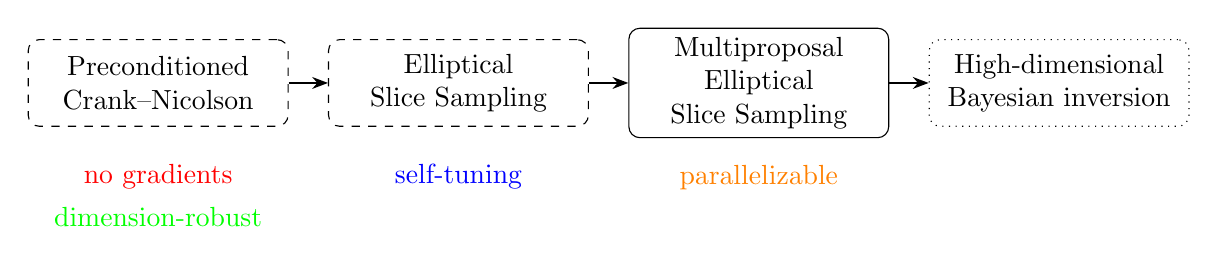
\begin{tikzpicture}[
    box/.style={draw, rounded corners, align=center, minimum height=1.1cm, minimum width=3.3cm},
    box-dashed/.style={box, dashed},
    box-dotted/.style={box, dotted},
    arrow/.style={-{Stealth[length=2mm]}, thick}
]
\onslide<2->{\node[box-dashed] (pcn) {Preconditioned\\Crank--Nicolson};}
\onslide<3->{\node[box-dashed, right=0.5cm of pcn] (ess) {Elliptical\\Slice Sampling};}
\onslide<4->{\node[box, right=0.5cm of ess] (mess) {Multiproposal\\Elliptical\\Slice Sampling};}
\onslide<5->{\node[box-dotted, right=0.5cm of mess] (inv) {High-dimensional\\Bayesian inversion};}

\onslide<3->{\draw[arrow] (pcn) -- (ess);}
\onslide<4->{\draw[arrow] (ess) -- (mess);}
\onslide<5->{\draw[arrow] (mess) -- (inv);}

\onslide<2->{\node[below=0.35cm of pcn] {\textcolor{red}{no gradients}};}
\onslide<2->{\node[below=0.9cm of pcn] {\textcolor{green}{dimension-robust}};}
\onslide<3->{\node[below=0.35cm of ess] {\textcolor{blue}{self-tuning}};}
\onslide<4->{\node[below=0.22cm of mess] {\textcolor{orange}{parallelizable}};}
\end{tikzpicture}
% }
\end{frame}

% --------------------------------
\section{Motivation and Background}

\begin{frame}{Motivation}
\begin{itemize}[<+->]
    \item Bayesian inverse problem
    \begin{equation*}
        \pi(x|\mathsf{y}) \propto \mathcal{L}(\mathsf{y}|x)\, \pi_0(x), \quad \mathsf{y} \in \mathbb{R}^k \text{ (observations)}, \quad x \in \mathbb{R}^d \text{ (parameters)}
    \end{equation*}
    \item Often non-parametric: 
    \begin{equation*}
        \quad \{x(s): s\in D\}, \quad D \subset \mathbb{R}^d.
    \end{equation*}
    \vspace{0.25em}
    \item Sampling with Markov models:
    \begin{itemize}
        \item Construct ergodic Markov chain $\bm{X}=\{X_1, X_2, \dots, X_N\}$ with $\pi$ as invariant measure.
        \vspace{0.25em}
        \item Approximate expectations:
        \[
            \lim_{N \to \infty} \frac{1}{N} \sum_{i=1}^N f(X_i) =  \hat{\mathbb{E}}_{\pi}[f(X)]
        \]
    \end{itemize}
    % \item Goal: Gradient-free algorithm for high-dimensional posteriors.
\end{itemize}
\end{frame}

% \section{Background}
% --------------------------------
\begin{frame}{Markov chain Monte Carlo (MCMC)}
\begin{algorithm}[H]
\caption{Metropolis-Hastings \citep{Hastings1970}}
\SetKwInOut{Input}{Input}
\Input{Current state $x$, likelihood $\mathcal{L}(\mathsf{y}|x)$, prior $\pi_0(x)$, proposal density $q$.}
\DontPrintSemicolon
1. Sample $x^{\star} = x + \nu, \quad \nu \sim q$\;
2. Compute acceptance probability 
\begin{equation*}
    \alpha(x, x^{\star}) = \min\{1, \frac{\mathcal{L}(\mathsf{y}|x^{\star})}{\mathcal{L}(\mathsf{y}|x)} \times \frac{\pi(x^{\star})}{\pi(x)} \times \frac{q(x|x^{\star})}{q(x^{\star}|x)}\}
\end{equation*}
3. Accept $x^{\star}$ with probability $\alpha(x, x^{\star})$, otherwise reject.\;
\end{algorithm}
\vspace{0.5cm}
\[
    \text{total cost}_{\varepsilon} = \text{cost per iteration} \times \text{number of iterations}_{\varepsilon}
\]
\begin{itemize}[<+->]
    \item Both increase with input size.
    % \item Challenge: cost and mixing degrade with dimension.

    % \item Construct an ergodic Markov chain $\bm{X}=\{X_1, X_2, \dots, X_N\}$ with $\pi$ as invariant measure.
    % \vspace{0.25em}
    % \item Approximate expectations via ergodic averages:
    % \[
    %     \lim_{N \to \infty} \frac{1}{N} \sum_{i=1}^N f(X_i) =  \hat{\mathbb{E}}_{\pi}[f(X)]
    % \]
    % \vspace{0.25em}
    % \item Metropolis-Hastings (MH) recipe:
    % \begin{itemize}[<+->]
    %     \item Assume $x \in \mathbb{R}^d$ and $\pi(x)$ is known up to a normalizing constant.
    %     \item Choose some proposal kernel $Q$ with density $q(x, y)$.
    %  \end{itemize}
\end{itemize}
\end{frame}

% \begin{frame}{Pre-conditioned Crank-Nicolson (pCN\footnote{\citet{Cotter2013,Neal1999}})}
% \begin{itemize}[<+->]
%     \item Target\footnote{\citet{stuart2010inverse}}: 
%     \[
%         \pi(x|\mathsf{y}) \propto \mathcal{L}(\mathsf{y}|x)\,\mathcal{N}(x;0,C).
%     \]
%     \vspace{0.25em}
%     \item Proposal:
%     \[
%         x^{\star} = \rho \, x + \sqrt{1-\rho^2}\,\nu,\quad \nu\sim N(0, C), \quad \rho \in (0,1) \Rightarrow \mbox{\textcolor{red}{no gradients}}.
%     \]
%     \vspace{0.25em}
%     \item Proposal keeps the prior invariant:
%         \[
%         q(x^{\star}|x) = \mathcal{N}(x^{\star}; \rho\,x, (1-\rho^2)C)
%     \]
%     \[
%         \mathcal{N}(x;0,C) \mathcal{N}(x^{\star}; \rho\,x, (1-\rho^2)C) = \mathcal{N}(x^{\star};0,C)\mathcal{N}(x; \rho\,x^{\star}, (1-\rho^2)C).
%     \]
%     \item Acceptance probability:
%     \[
%         \alpha(x,x^{\star}) = \min\{1, \frac{\mathcal{L}(\mathsf{y}|x^{\star})}{\mathcal{L}(\mathsf{y}|x)}\} \to \mbox{\textcolor{green}{dimension-free}}
%     \]
% \end{itemize}
% \end{frame}

\begin{frame}{Pre-conditioned Crank-Nicolson (PCN)}
\onslide<1->{
Posterior distribution\footnote{\citet{stuart2010inverse,Dashti2013TheBA}}:
\[
    \pi(x|\mathsf{y}) \propto \mathcal{L}(\mathsf{y}|x)\,\mathcal{N}(x;0,C).
\]
}
% \vspace{0.2em}
\onslide<2->{
\begin{algorithm}[H]
\caption{PCN \citep{Cotter2013,Neal1999}}
\SetKwInOut{Input}{Input}
\Input{Current state $x$, agressiveness $\rho\in(0,1)$}
\DontPrintSemicolon
1. Propose $x^{\star} = \rho \, x + \sqrt{1-\rho^2}\,\nu,\quad \nu\sim \mathcal{N}(0, C)$ {\scriptsize \textcolor{red}{no gradients}}\;
2. Compute $\alpha(x,x^{\star})=\min\{1,\mathcal{L}(\mathsf{y}|x^{\star})/\mathcal{L}(\mathsf{y}|x)\}$\;
3. Accept $x^{\star}$ with probability $\alpha(x,x^{\star})$, otherwise reject.\;
\end{algorithm}
}
\vspace{0.2cm}
\onslide<3->{
Proposal is reversible with respect to the prior: 
\[
    \mathcal{N}(x^{\star};0,C)\mathcal{N}(x; \rho\,x^{\star}, (1-\rho^2)C) = \mathcal{N}(x;0,C) \mathcal{N}(x^{\star}; \rho\,x, (1-\rho^2)C) \quad\quad\quad\Rightarrow \mbox{\textcolor{green}{dimension-free}}
\]
}
\end{frame}

\begin{frame}{Elliptical Slice Sampling (ESS)\footnote{\citet{Murray2010}}}
\begin{figure}
    \centering
    \begin{subfigure}[b]{0.45\linewidth}
        \centering
        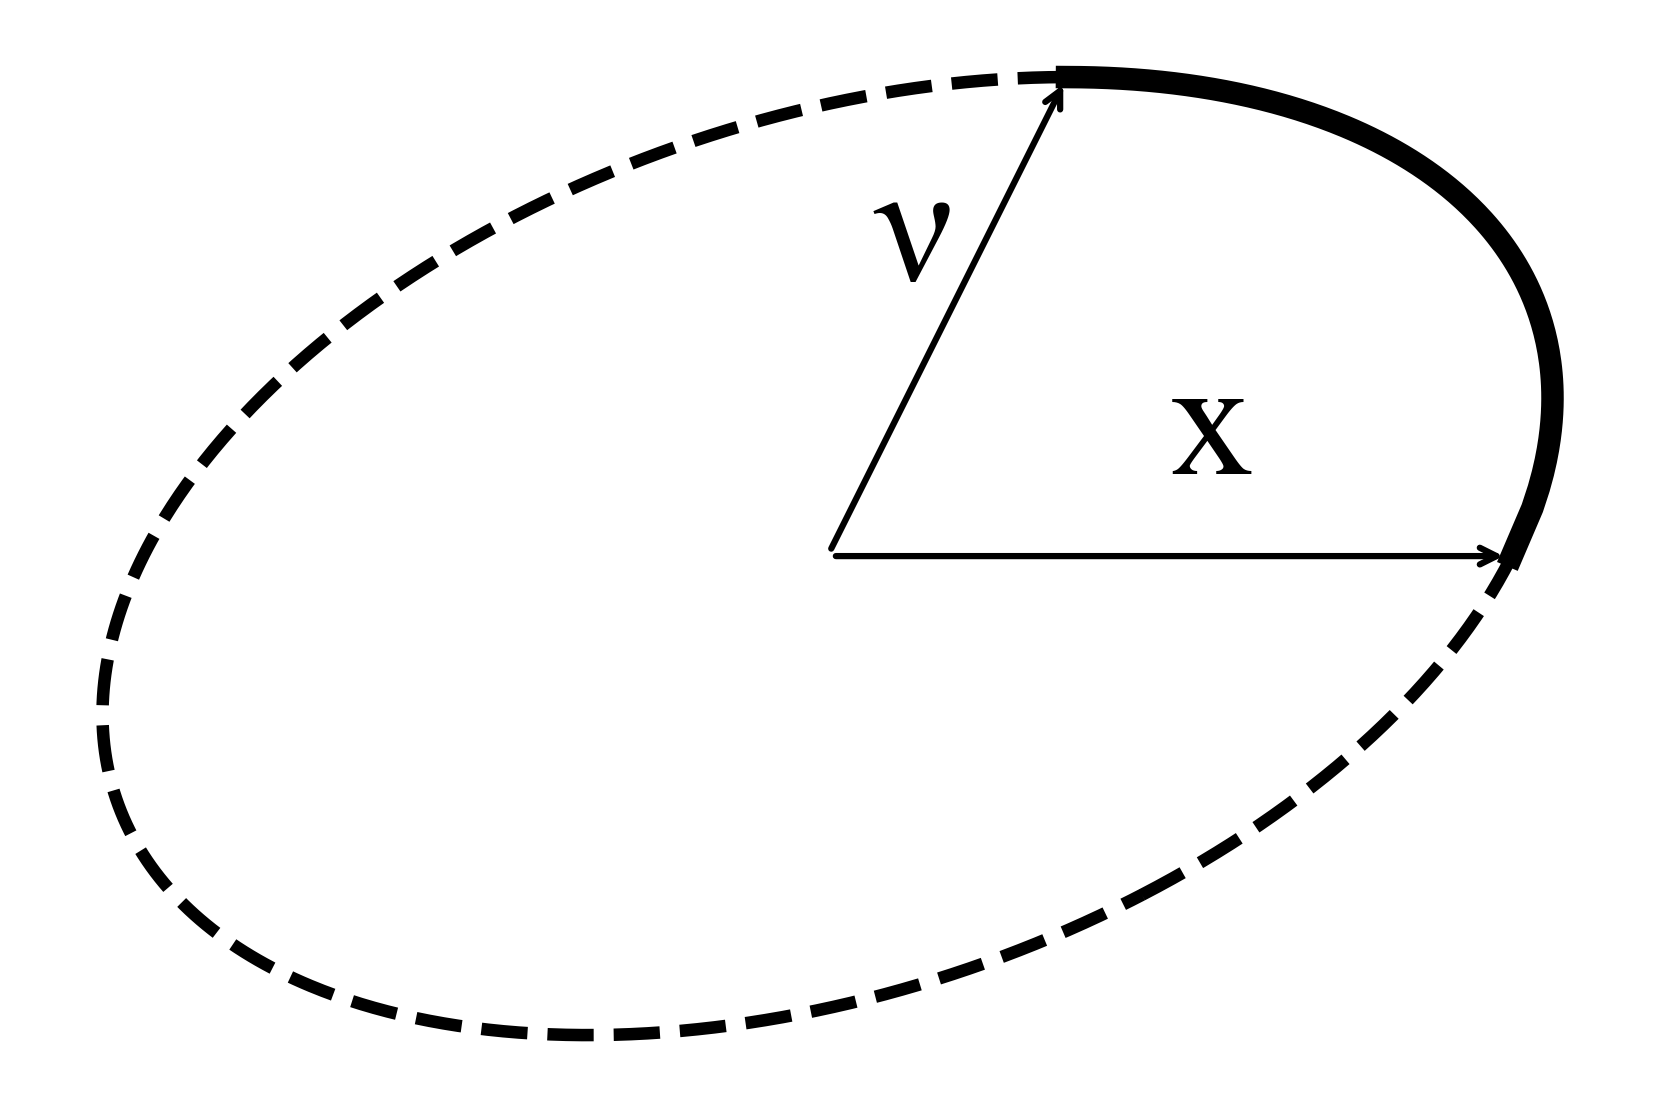
\includegraphics[width=0.4\linewidth]{pcn_locus_ellipse.png}
        \caption{PCN: $x^{\star} = \rho \, x + \sqrt{1-\rho^2}\,\nu, \quad \rho \in (0, 1)$}
    \end{subfigure}
    \hfill
    \begin{subfigure}[b]{0.45\linewidth}
        \centering
        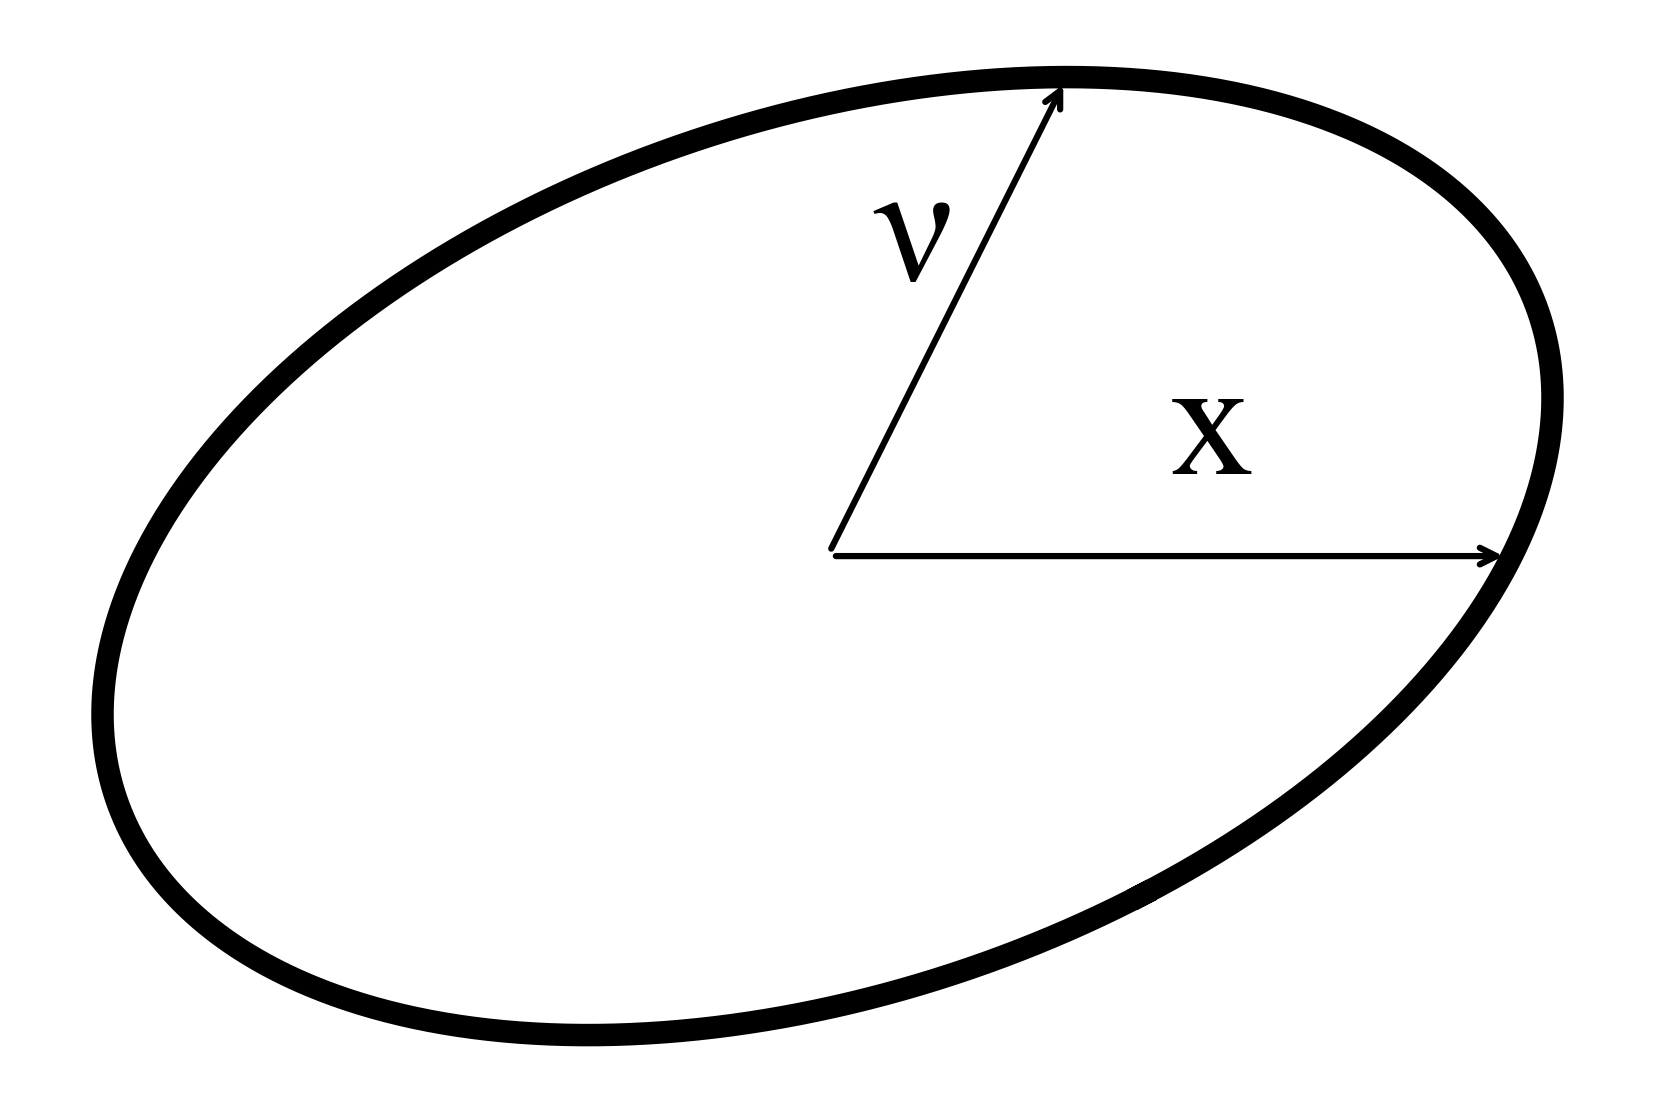
\includegraphics[width=0.4\linewidth]{ess_locus_ellipse.png}
        \caption{ESS proposal}
    \end{subfigure}
\end{figure}
    \begin{itemize}[<+->]
    % \item Posterior defined by
    % \[
    %     \pi(x|\mathsf{y}) \propto \mathcal{L}(\mathsf{y}|x)\,\mathcal{N}(x; \mu, \Sigma).
    % \]
    % \vspace{0.25em}
    \item Elliptical proposal:
    \[
        x^{\star} = x \cos\theta + \nu \sin\theta,\quad \nu\sim\mathcal{N}(0,C), \quad \theta \in (0, 2\pi].
    \]
    % \begin{itemize}
    %     \item Keeps prior invariant.
    % \end{itemize}
    % \[
    %     q(x, x^{\star}) = \mathcal{N}(x^{\star}; x \cos \theta, \sin^2 \theta \, C)
    % \]
    % keeps the prior invariant for any $\theta$:
    % \item Acceptance probability:
    % \[
    %     \alpha(x,x^{\star}) = \min\{1, \frac{\mathcal{L}(\mathsf{y}|x^{\star})}{\mathcal{L}(\mathsf{y}|x)}\} \to \mbox{\textcolor{green}{dimension-free}}
    % \]    
    % \vspace{0.5cm}
    \item Holds the prior invariant.
    \item Choose $\rho$ automatically $\to \mbox{\textcolor{blue}{self-tuning}}$.
\end{itemize}
\end{frame}

\begin{frame}{Slice Sampling}

\begin{columns}[t]

\begin{column}{0.5\textwidth}
\onslide<1->{
\vfill
\begin{itemize}
    % \item Augmented variable method.
    \item Idea:
    \[
    \pi(x,y)=
    \begin{cases}
    \frac{1}{\int f(x)\,dx} & 0<y<f(x) \\
    0 & \text{otherwise}
    \end{cases}
    \]
\end{itemize}
\vfill
}
\onslide<2->{
\vspace{0.5cm}
\begin{algorithm}[H]
\caption{Slice sampling \citep{Neal2003}}
\DontPrintSemicolon
1. Sample $y \sim \mathcal{U}(0,f(x))$\;
2. Sample $x\sim \mathcal{U}(\textcolor{olive}{\mathcal{S}})$\;
\end{algorithm}
\vfill
}
\end{column}

\begin{column}{0.5\textwidth}
\onslide<3->{
\vspace{-0.5cm}
\begin{figure}
\centering
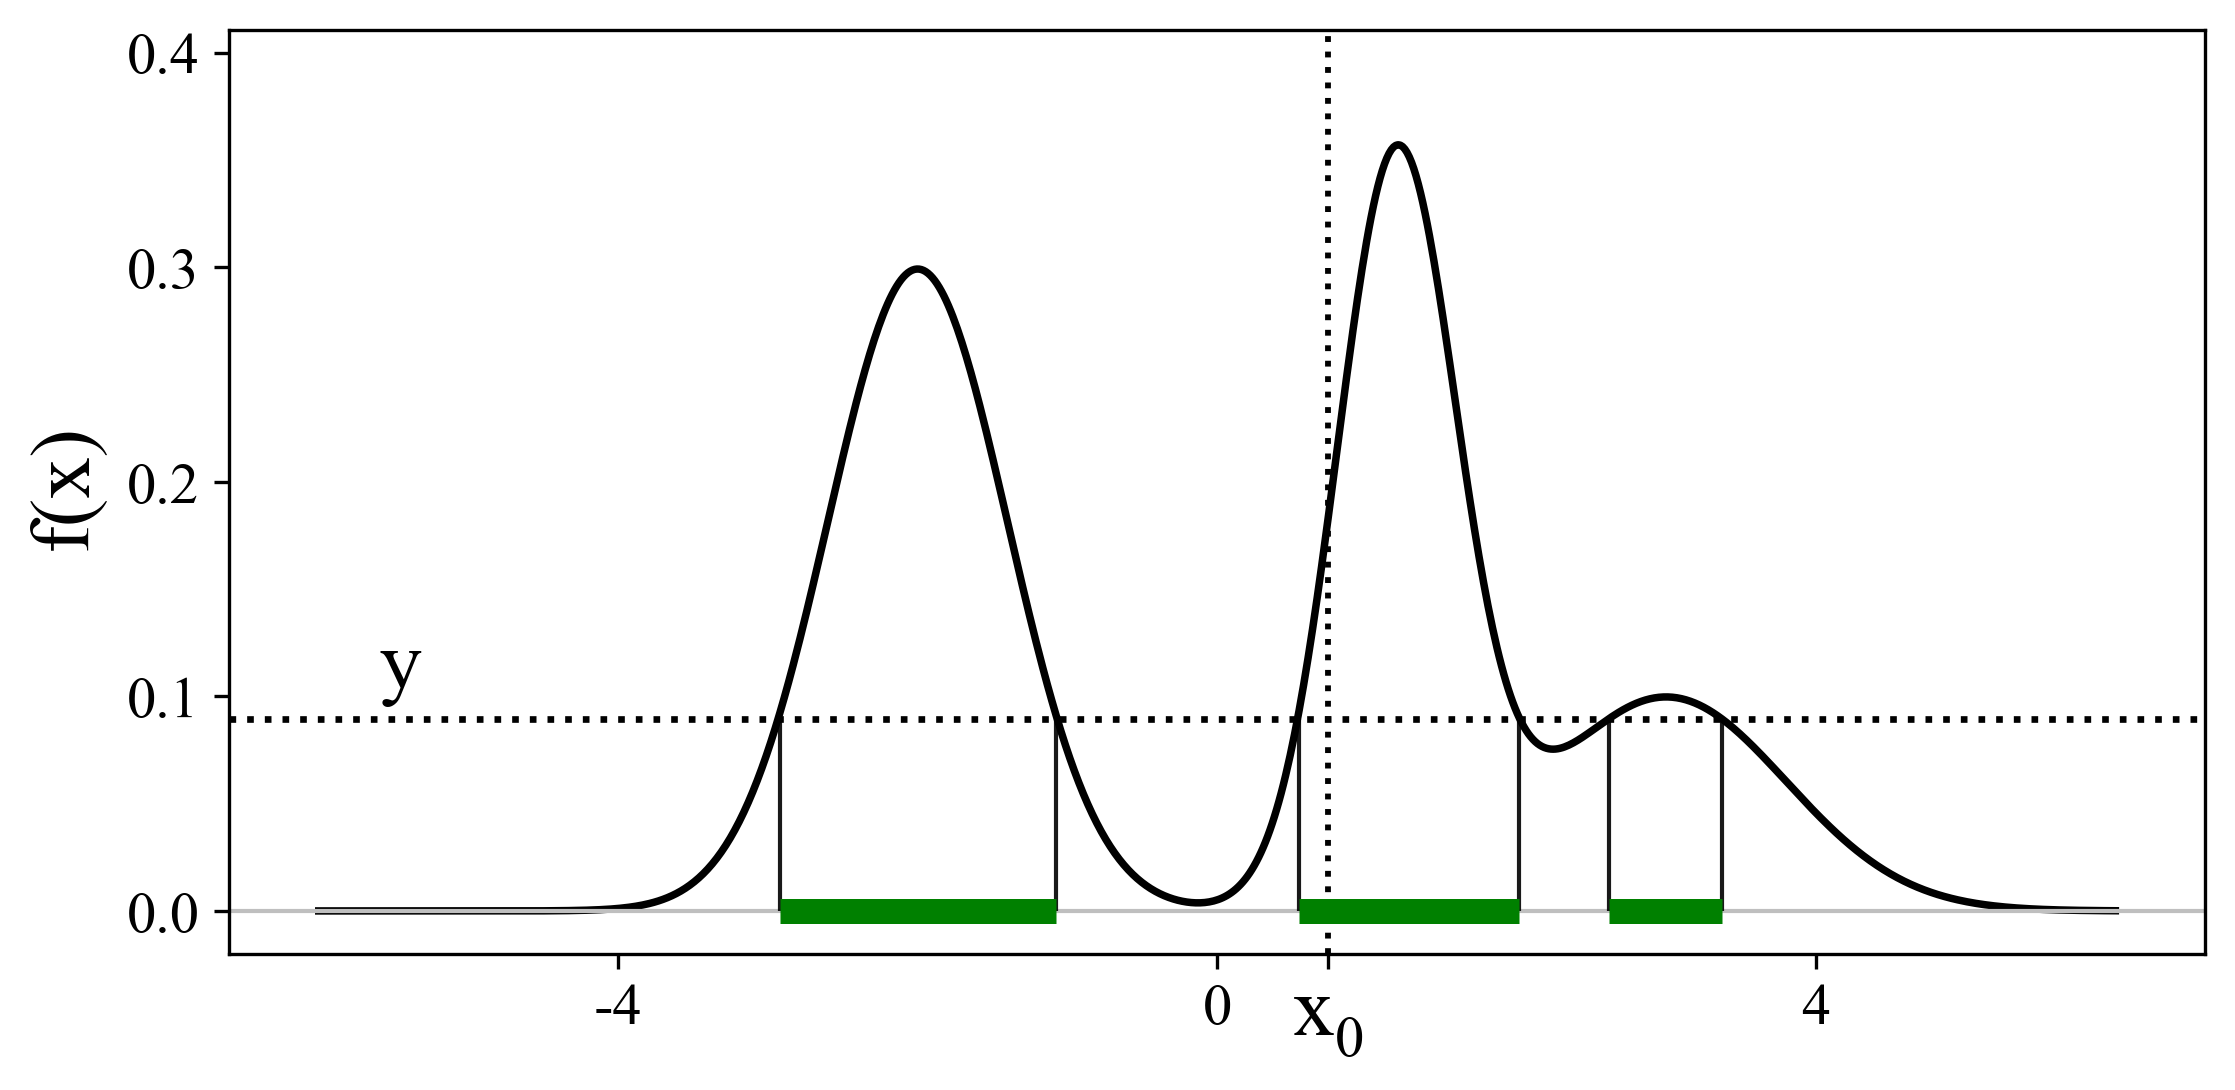
\includegraphics[width=1\linewidth]{slice_sampling_multimodal_x0.png}
\caption{\textit{ slice } sampling: $\textcolor{olive}{\mathcal{S}}=\{x:f(x)\ge y\}$}
\end{figure}
}

\end{column}

\end{columns}
\end{frame}


\begin{frame}{Shrinking}
\begin{itemize}[<+->]
    \item How to sample $x$ on $\mathcal{S}$ when $\mathcal{S}$ is unknown?
    \item Sample $x \sim \mathcal{U}(I)$. While $f(x) < y$, shrink $I$ around $x$.
    % \item Solution: Start from an interval $I \supset S$ and iteratively shrink until $x$ falls on $S$. 
\end{itemize}
\begin{figure}
    \centering
    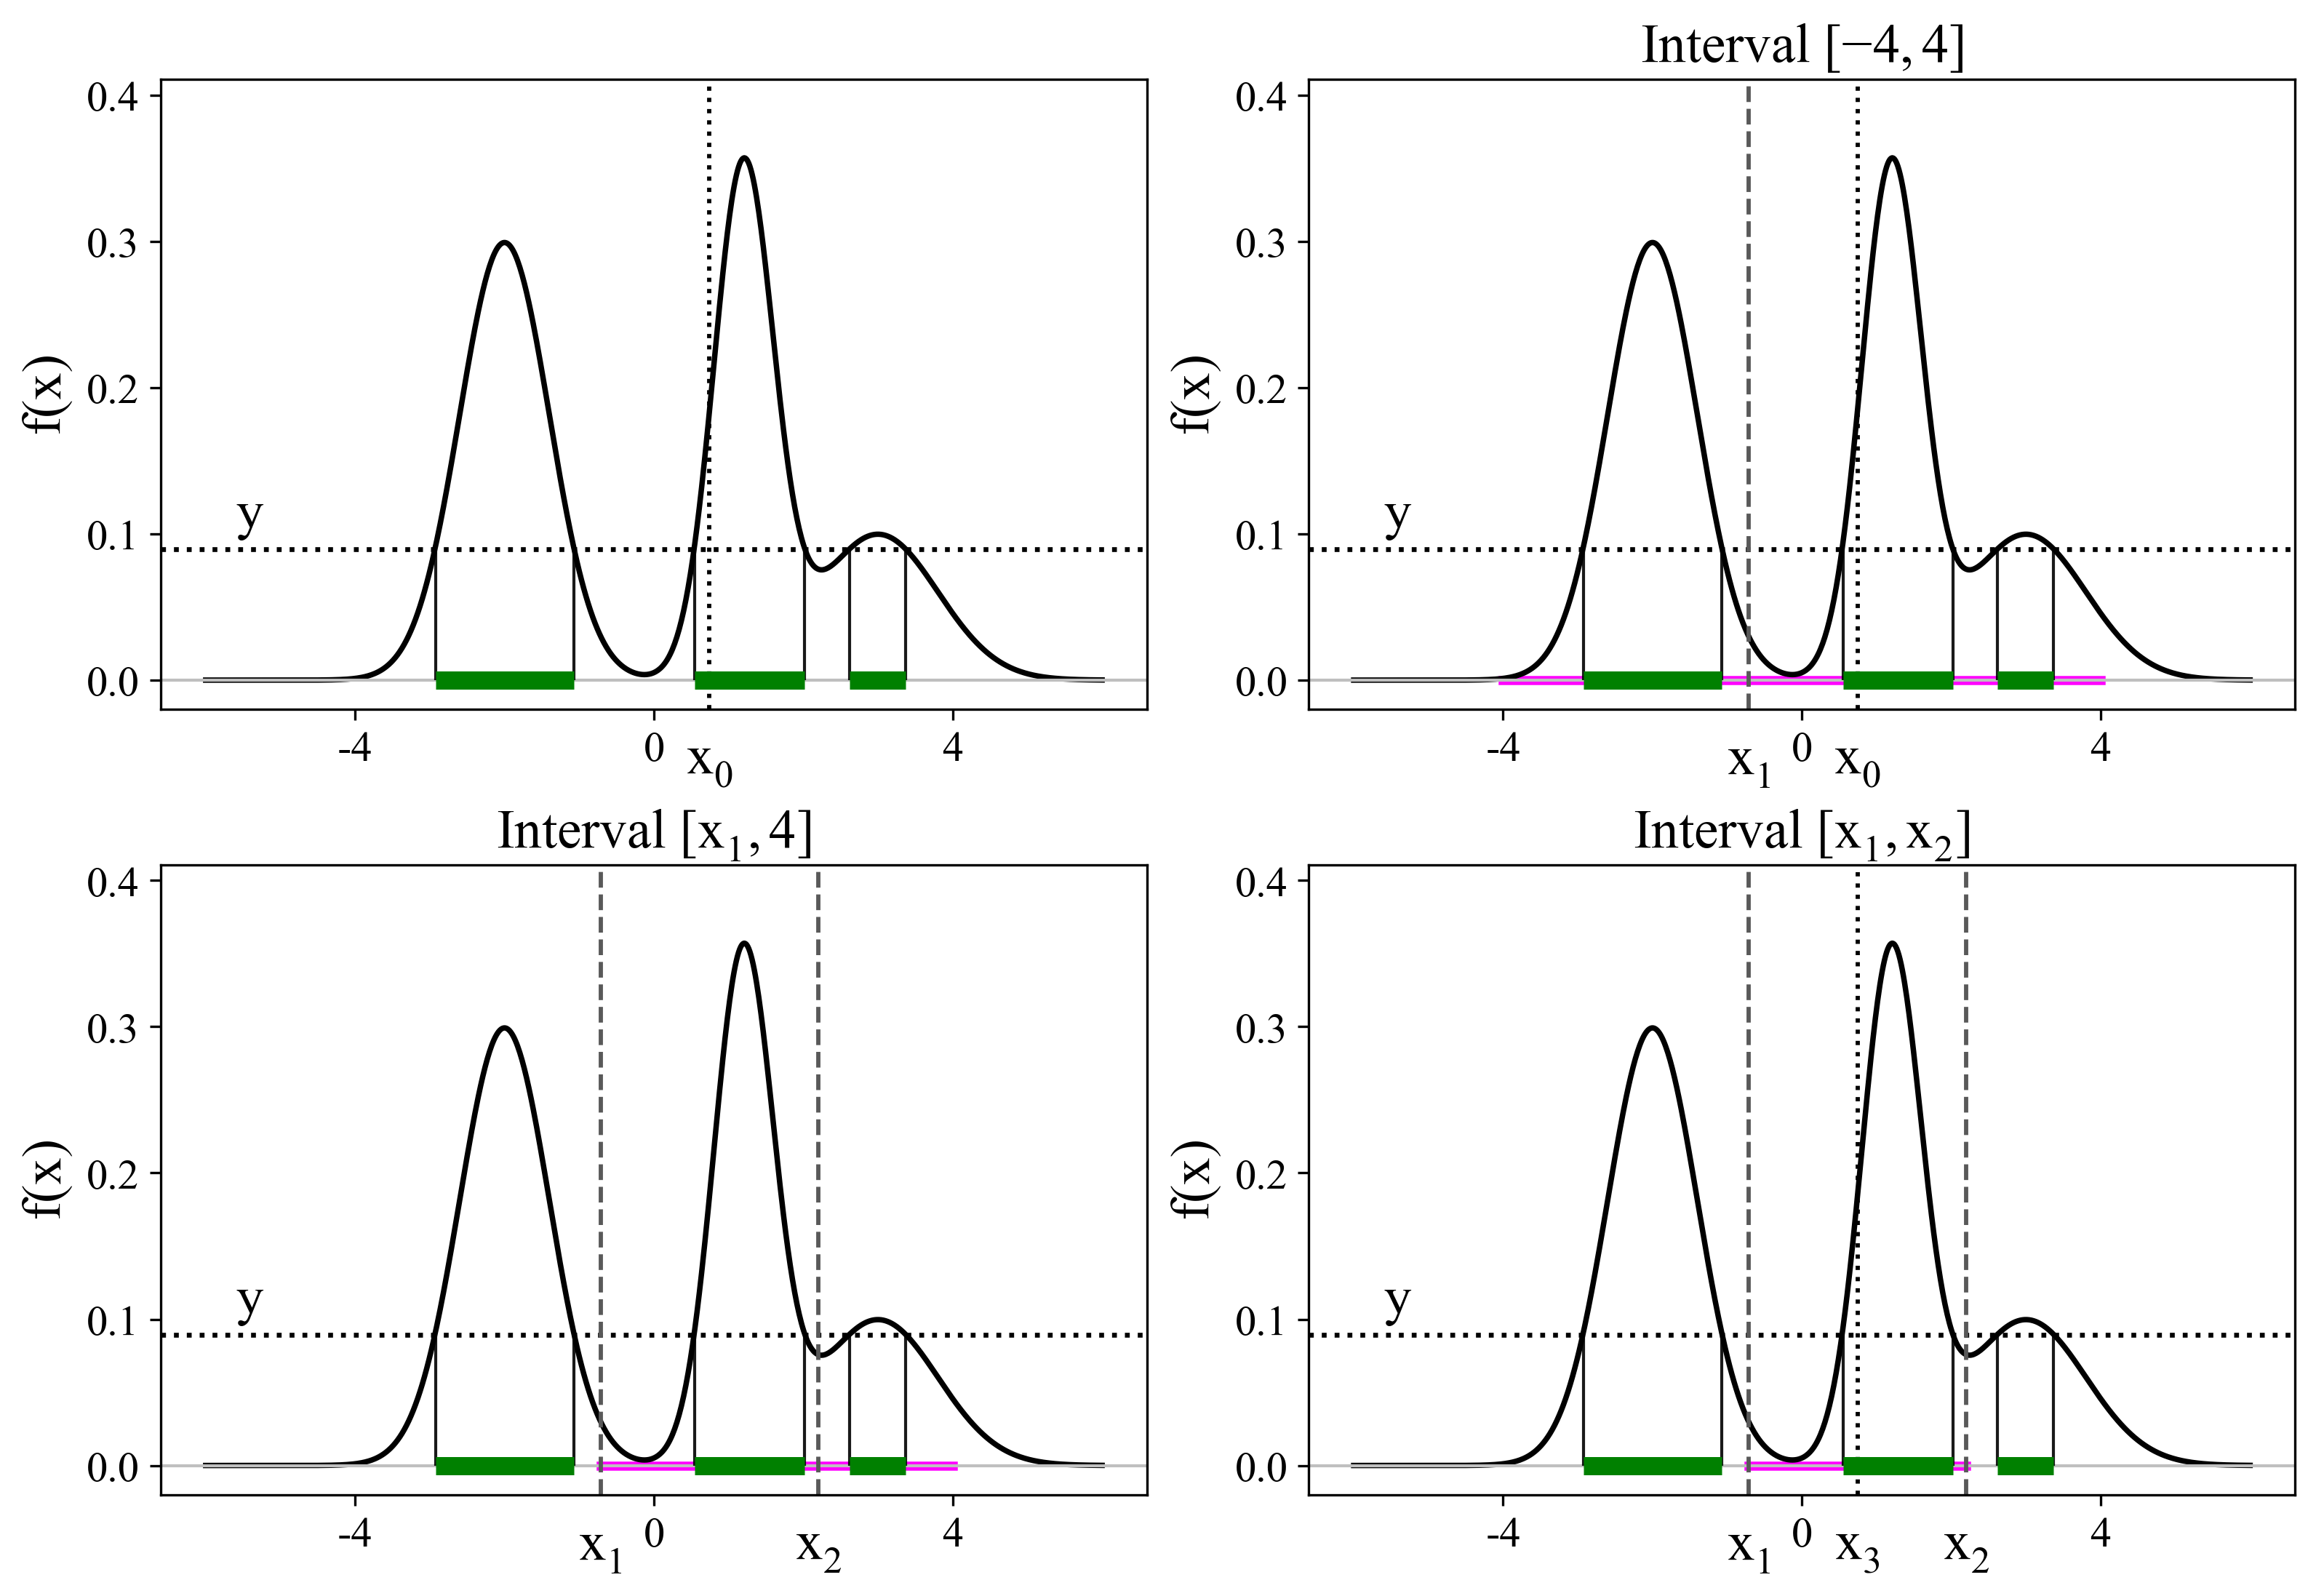
\includegraphics[width=0.5\linewidth]{slice_sampling_multimodal_sequence.png}
    % \caption{Shrinking the interval $I$ until it hits the slice $S$.}
\end{figure}  
\end{frame}

% \begin{frame}{Elliptical Slice Sampling (continued))}
% \begin{columns}
% \begin{column}{0.5\textwidth}
% \begin{itemize}[<+->]
%     \item Recall:
%     \begin{equation*}
%         x^{\star}(\theta) = x \cos\theta + \nu \sin\theta; \quad \alpha(x,x^{\star}) = \min\{1, \frac{\mathcal{L}(\mathsf{y}|x^{\star})}{\mathcal{L}(\mathsf{y}|x)}\}.
%     \end{equation*}
% \end{itemize}
% \begin{enumerate}[<+->]
%     \item Auxiliary variable $y$ defines the slice:
%     \[
%         y \sim \mathcal{U}(0, \mathcal{L}(\alpha)) \Rightarrow y = u\,\mathcal{L}(\alpha), \quad u \sim \mathcal{U}(0,1).
%     \]
%     \vspace{0.25em}

%     \item Sample $\theta^{(1)}$ uniformly and shrink, i.e. $\theta^{(1)}, \theta^{(2)}, \theta^{(3)}, \ldots$ until $\mathcal{L}(\theta^{(k)}) \ge y$ $\Rightarrow$ \textcolor{blue}{self-tuning}.
% \end{enumerate}
% \end{column}
% \begin{column}{0.5\textwidth}
%     \begin{figure}
%     \centering
%     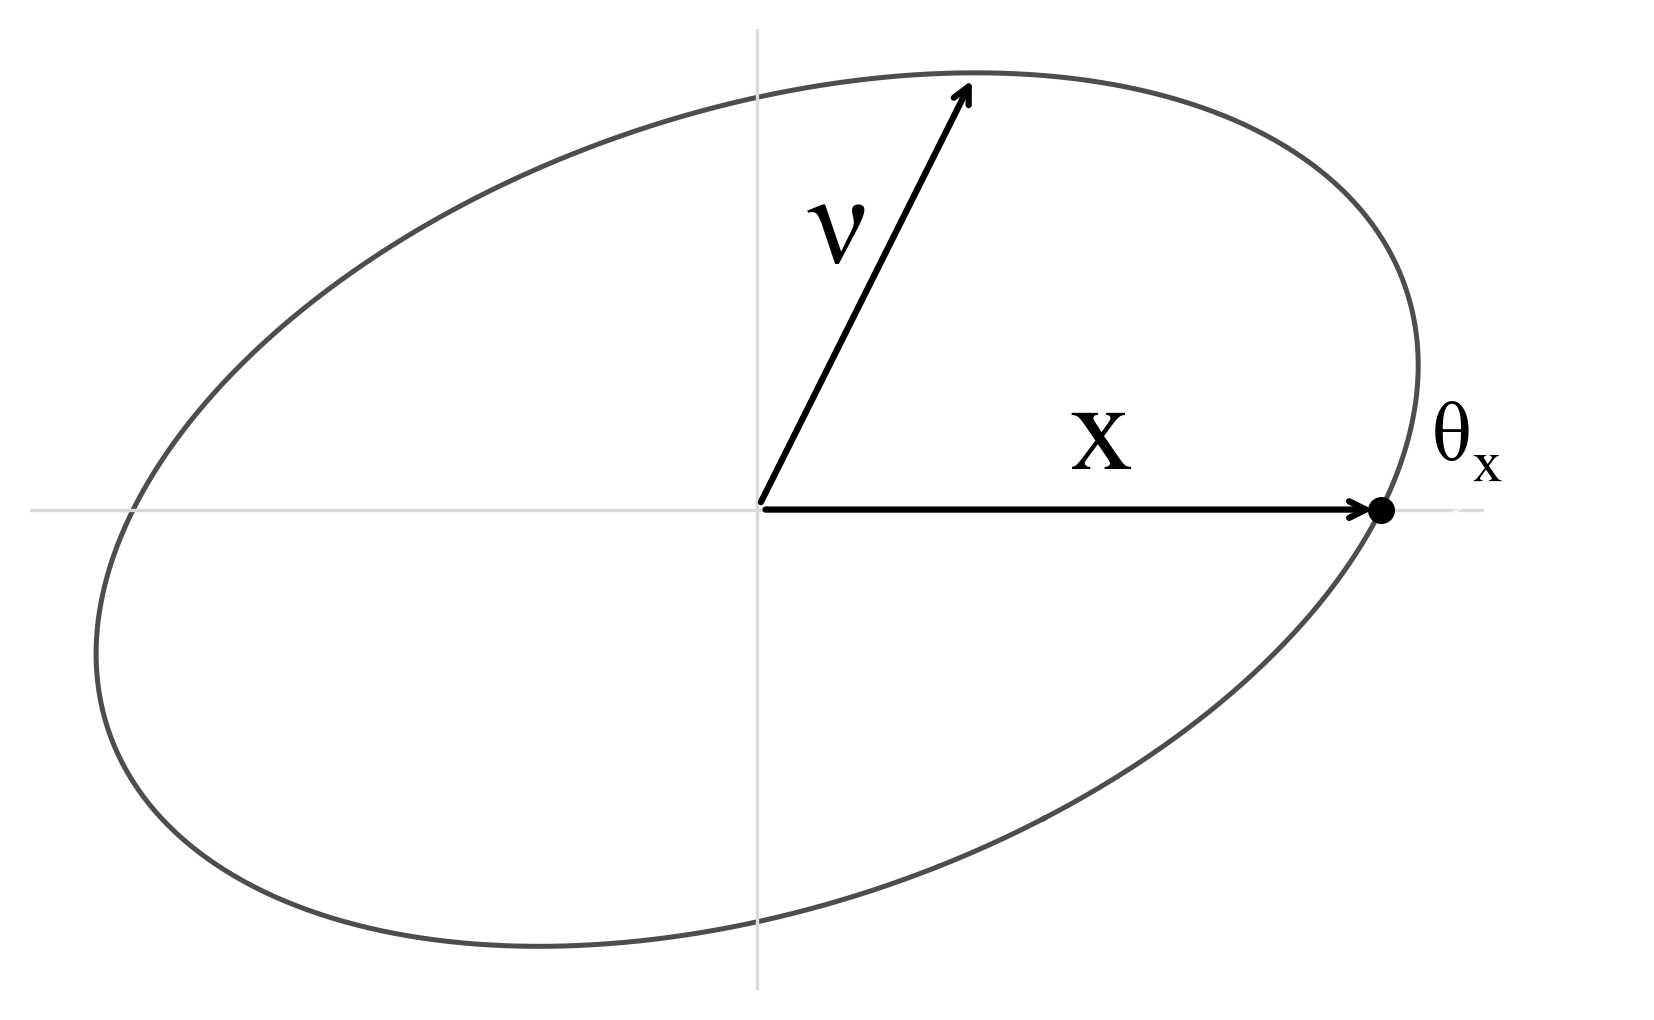
\includegraphics[width=0.3\linewidth]{ess_ellipse_one_proposal_nolabel_noslice.png}
%     % \caption{ESS proposal with slice.}
%     \end{figure}
%     \begin{figure}
%     \centering
%     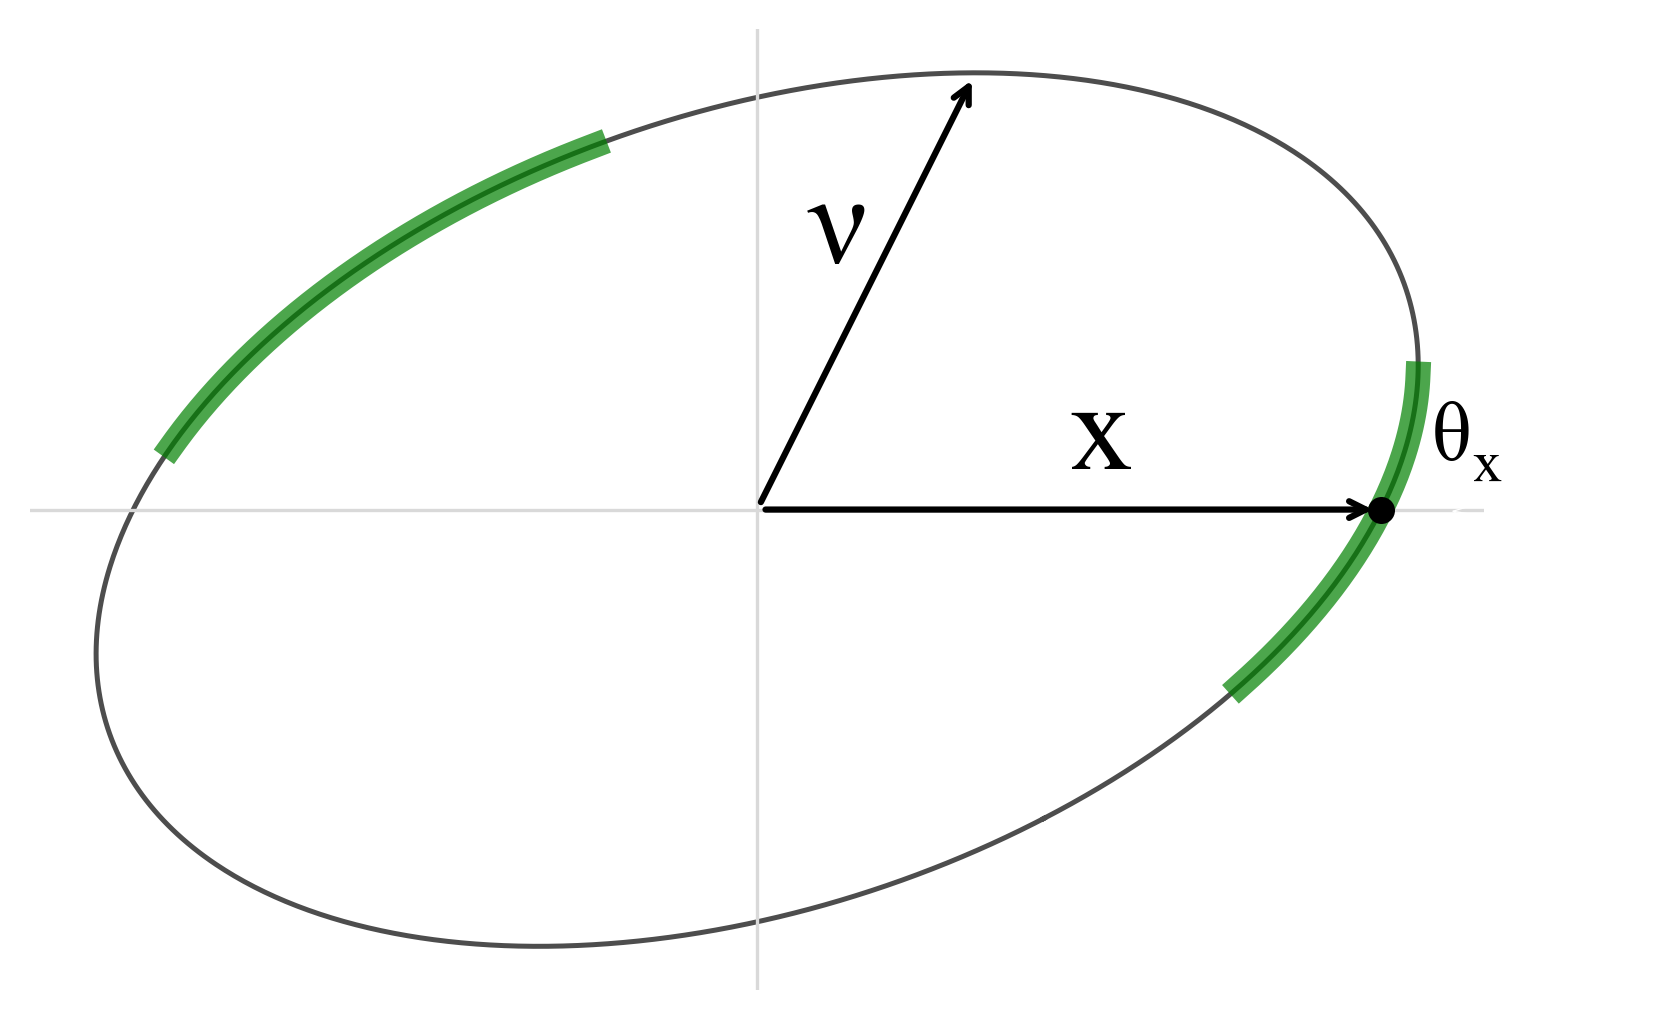
\includegraphics[width=0.3\linewidth]{ess_ellipse_one_proposal_nolabel.png}
%     % \caption{ESS proposal with slice.}
%     \end{figure}
%     \begin{figure}
%     \centering
%     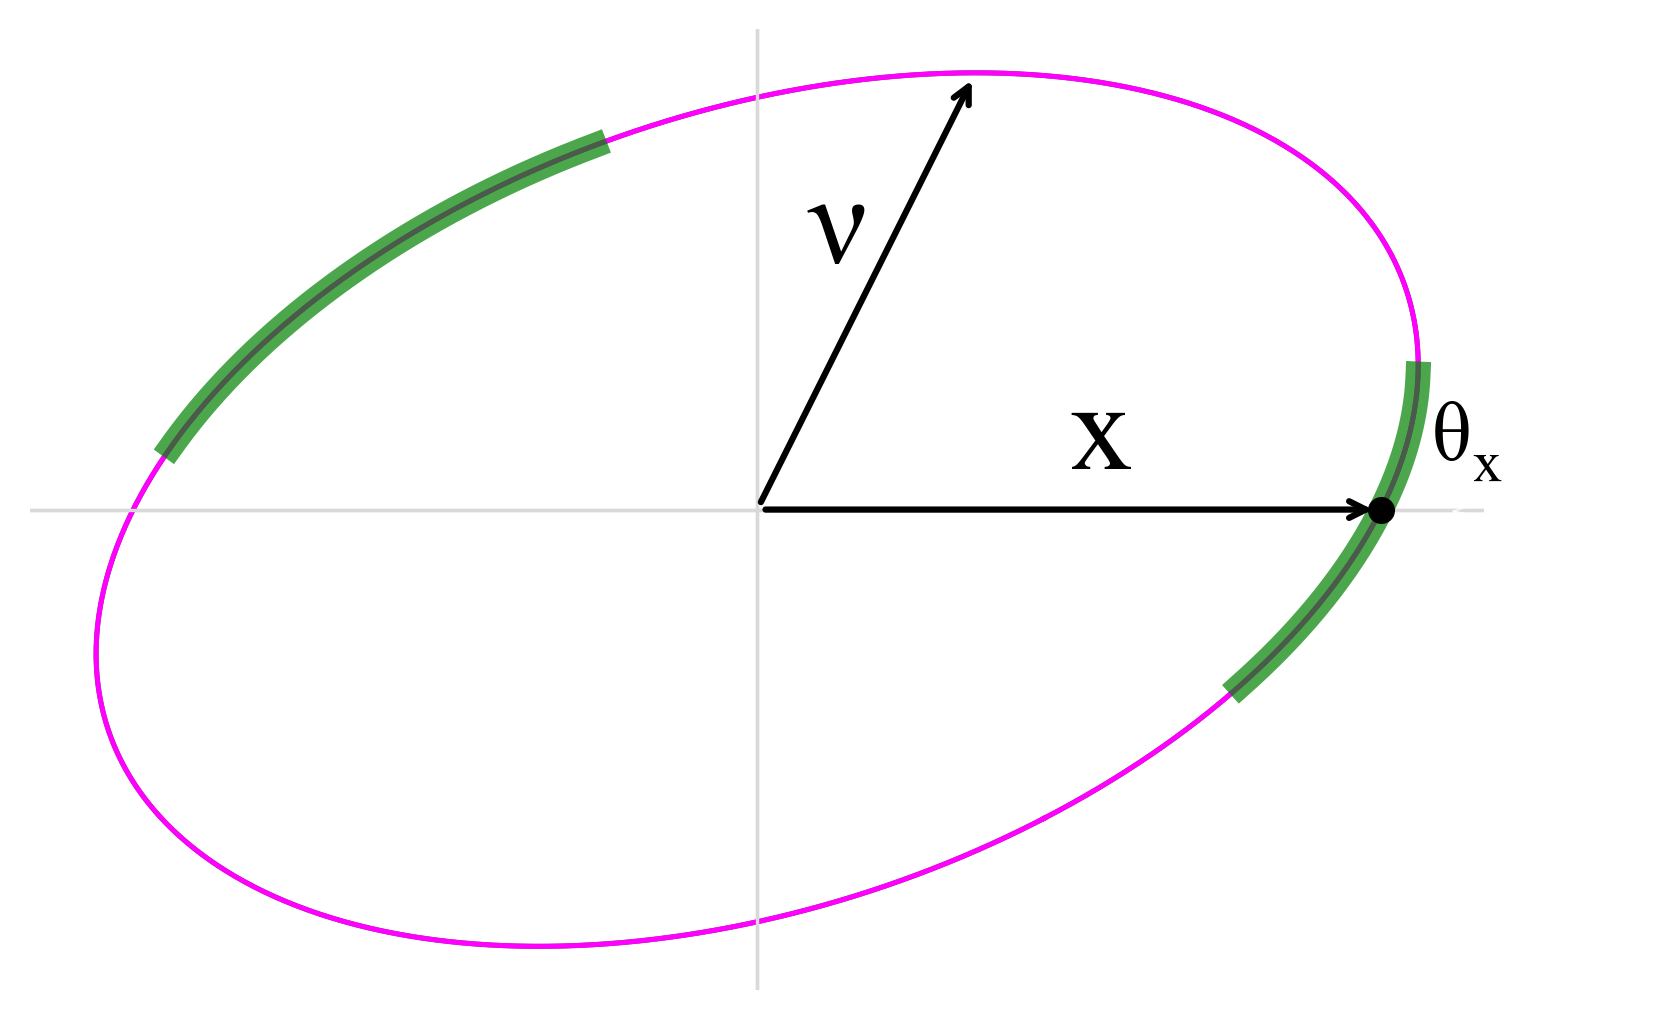
\includegraphics[width=0.3\linewidth]{ess_ellipse_one_proposal_pinkinterval.png}
%     % \caption{ESS proposal with slice.}
%     \end{figure}
%     \begin{figure}
%     \centering
%     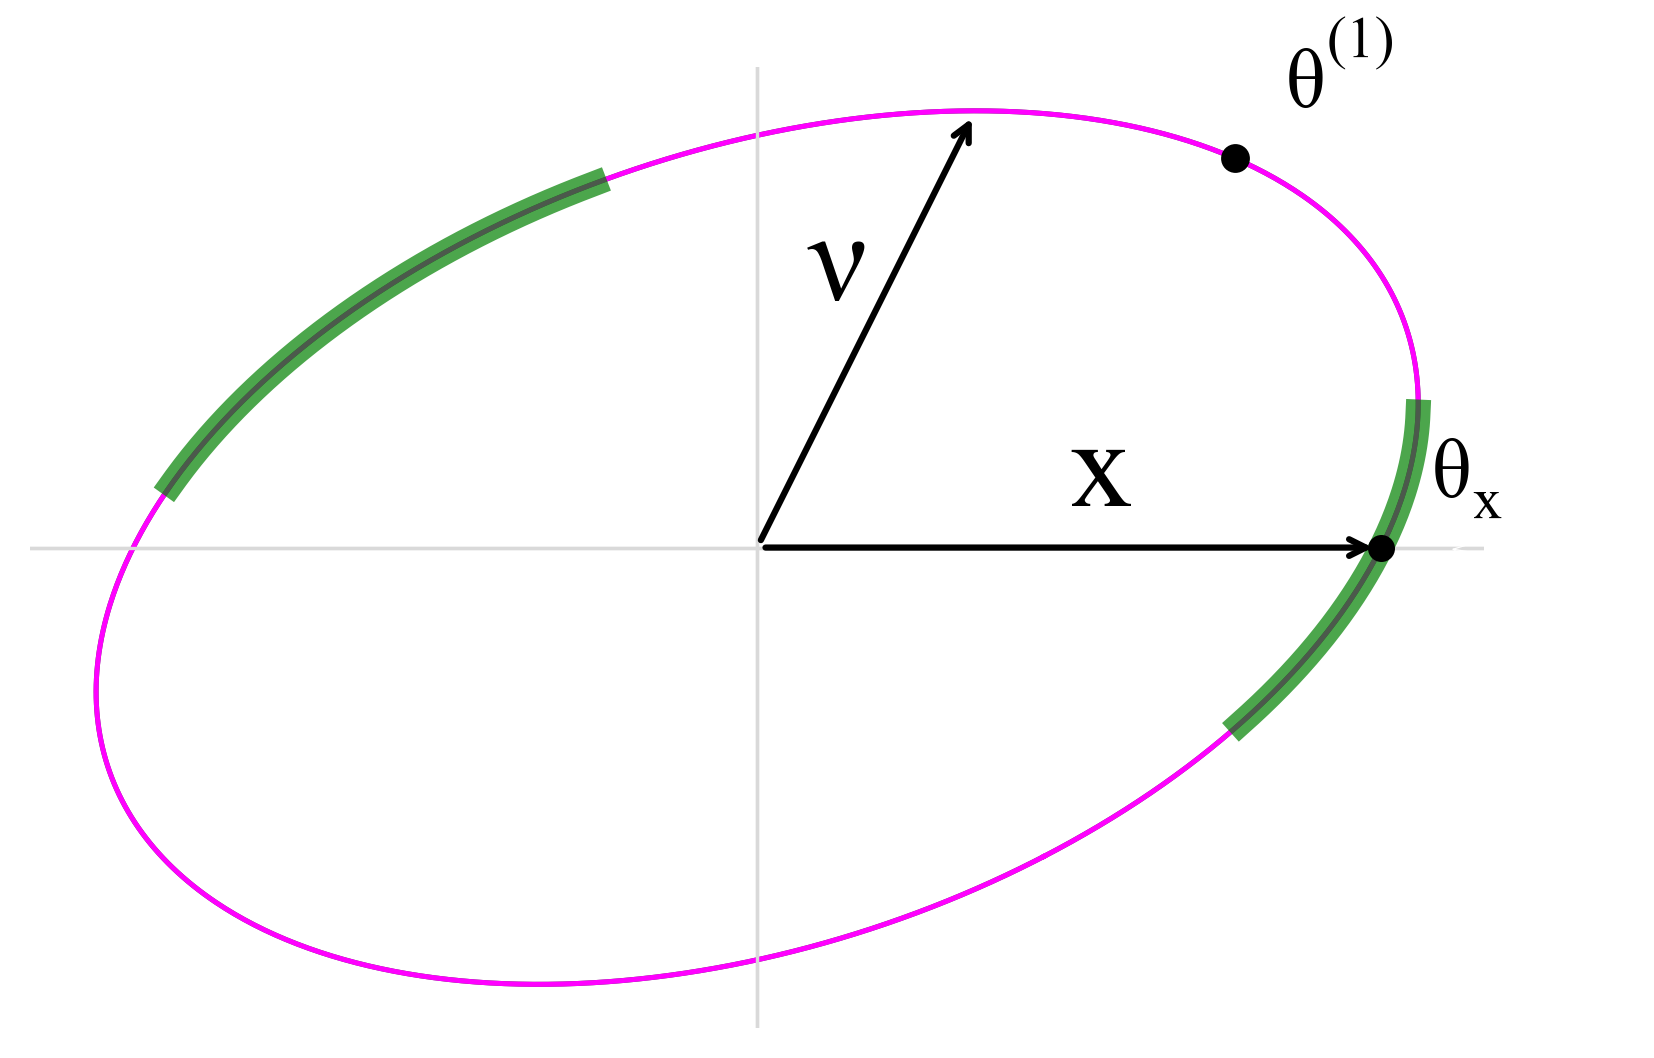
\includegraphics[width=0.3\linewidth]{ess_ellipse_one_proposal.png}
%     % \caption{ESS proposal with slice.}
%     \end{figure}
% \end{column}
% \end{columns}
% \end{frame}

\begin{frame}{Elliptical Slice Sampling (continued)}
\begin{columns}
\begin{column}{0.6\textwidth}
\begin{algorithm}[H]
\caption{ESS}
\SetKwInOut{Input}{Input}
\Input{Current state $x$.}
\DontPrintSemicolon
Draw $\nu\sim\mathcal{N}(0,C)$, defining the ellipse\;
Draw $\theta_x \sim \mathcal{U}(0, 2\pi)$\;
Draw slice level $y \sim \mathcal{U}(0, \mathcal{L}(\mathsf{y}|x))$\;
Set $\theta_{\text{min}} \gets 0$, $\theta_{\text{max}} \gets 2\pi$\;
\While{$\mathcal{L}(\mathsf{y}|x^{\star}) < y$}{
    Sample $\theta\sim\mathcal{U}(\theta_{\text{min}},\theta_{\text{max}})$\;
    Propose $x^{\star}=x\cos\theta + \nu\sin\theta$\;
    Evaluate $\mathcal{L}(\mathsf{y}|x^{\star})$\;
    Shrink $(\theta_{\text{min}},\theta_{\text{max}})$ around $\theta_x$\;
}
Accept $x\leftarrow x^{\star}$\;
% \While{true}{
%     Sample $\theta\sim\mathcal{U}(\theta_{\text{min}},\theta_{\text{max}})$\;
%     Propose $x^{\star}=x\cos\theta + \nu\sin\theta$\;
%     \If{$\mathcal{L}(\mathsf{y}|x^{\star})\ge y$}{accept $x\leftarrow x^{\star}$ and stop\;}
%     \Else{shrink $(\theta_{\text{min}},\theta_{\text{max}})$ around $\theta_x$ and continue {\scriptsize \textcolor{blue}{self-tuning}}\;}
% }
\end{algorithm}
\end{column}
\begin{column}{0.4\textwidth}
    \begin{figure}
    \centering
    \only<2>{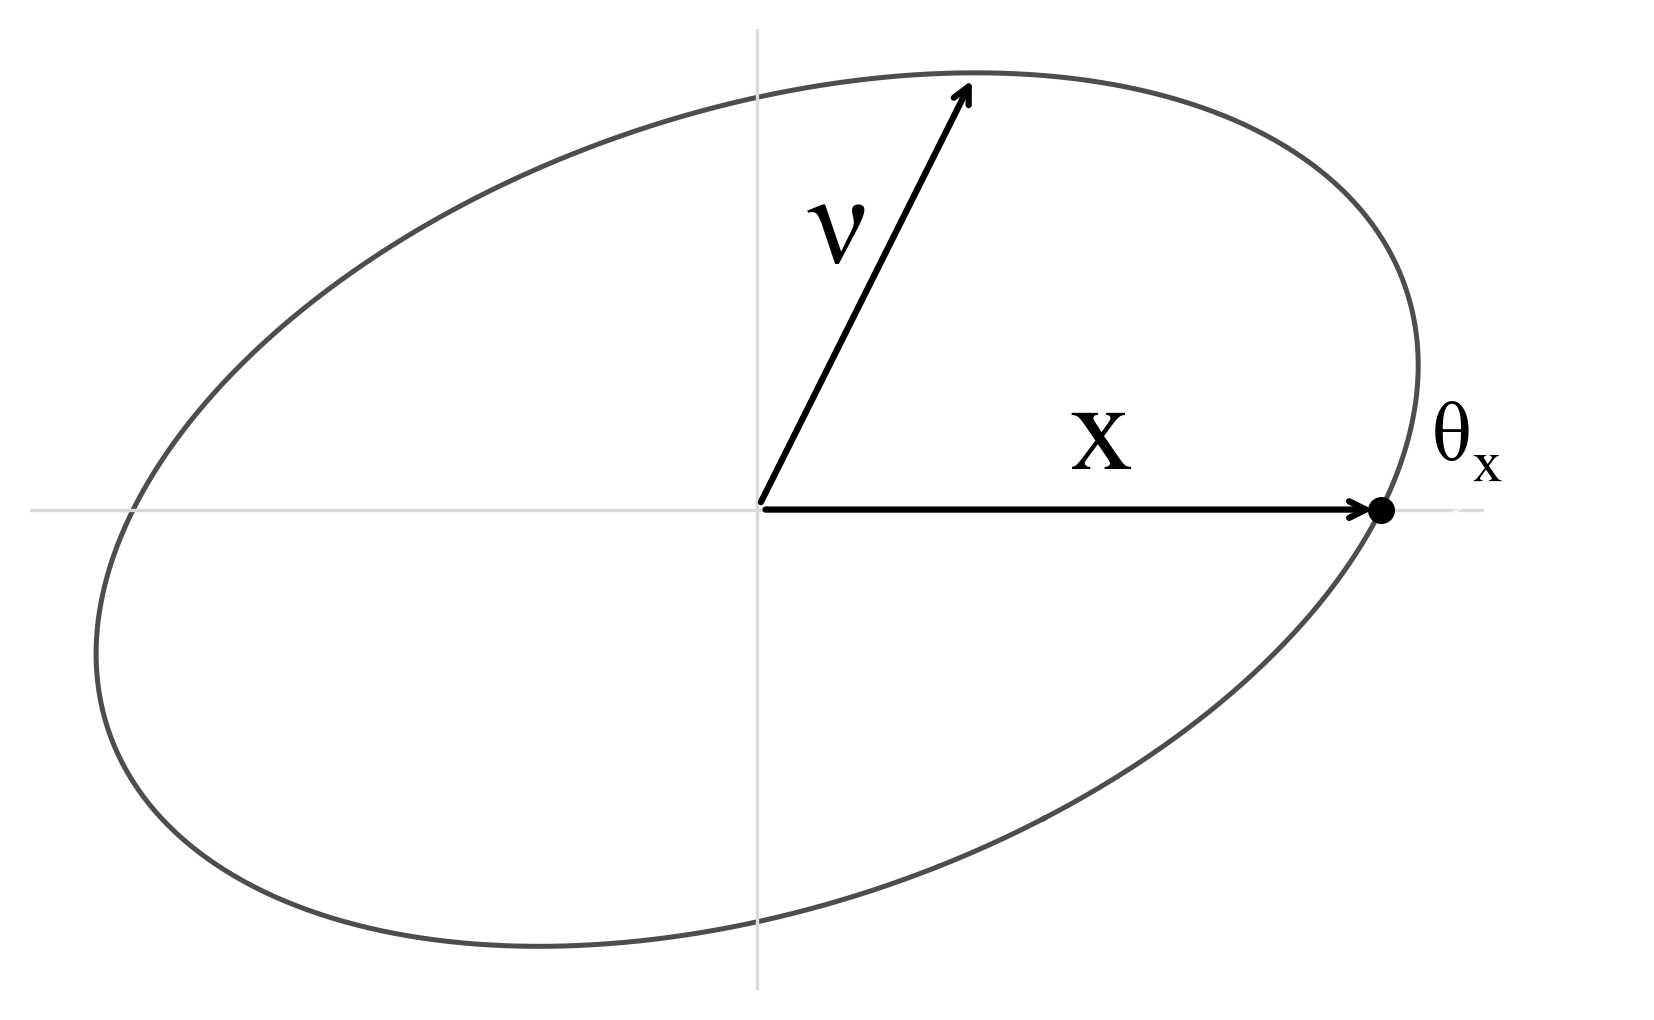
\includegraphics[width=0.7\linewidth]{ess_ellipse_one_proposal_nolabel_noslice.png}}
    \only<3>{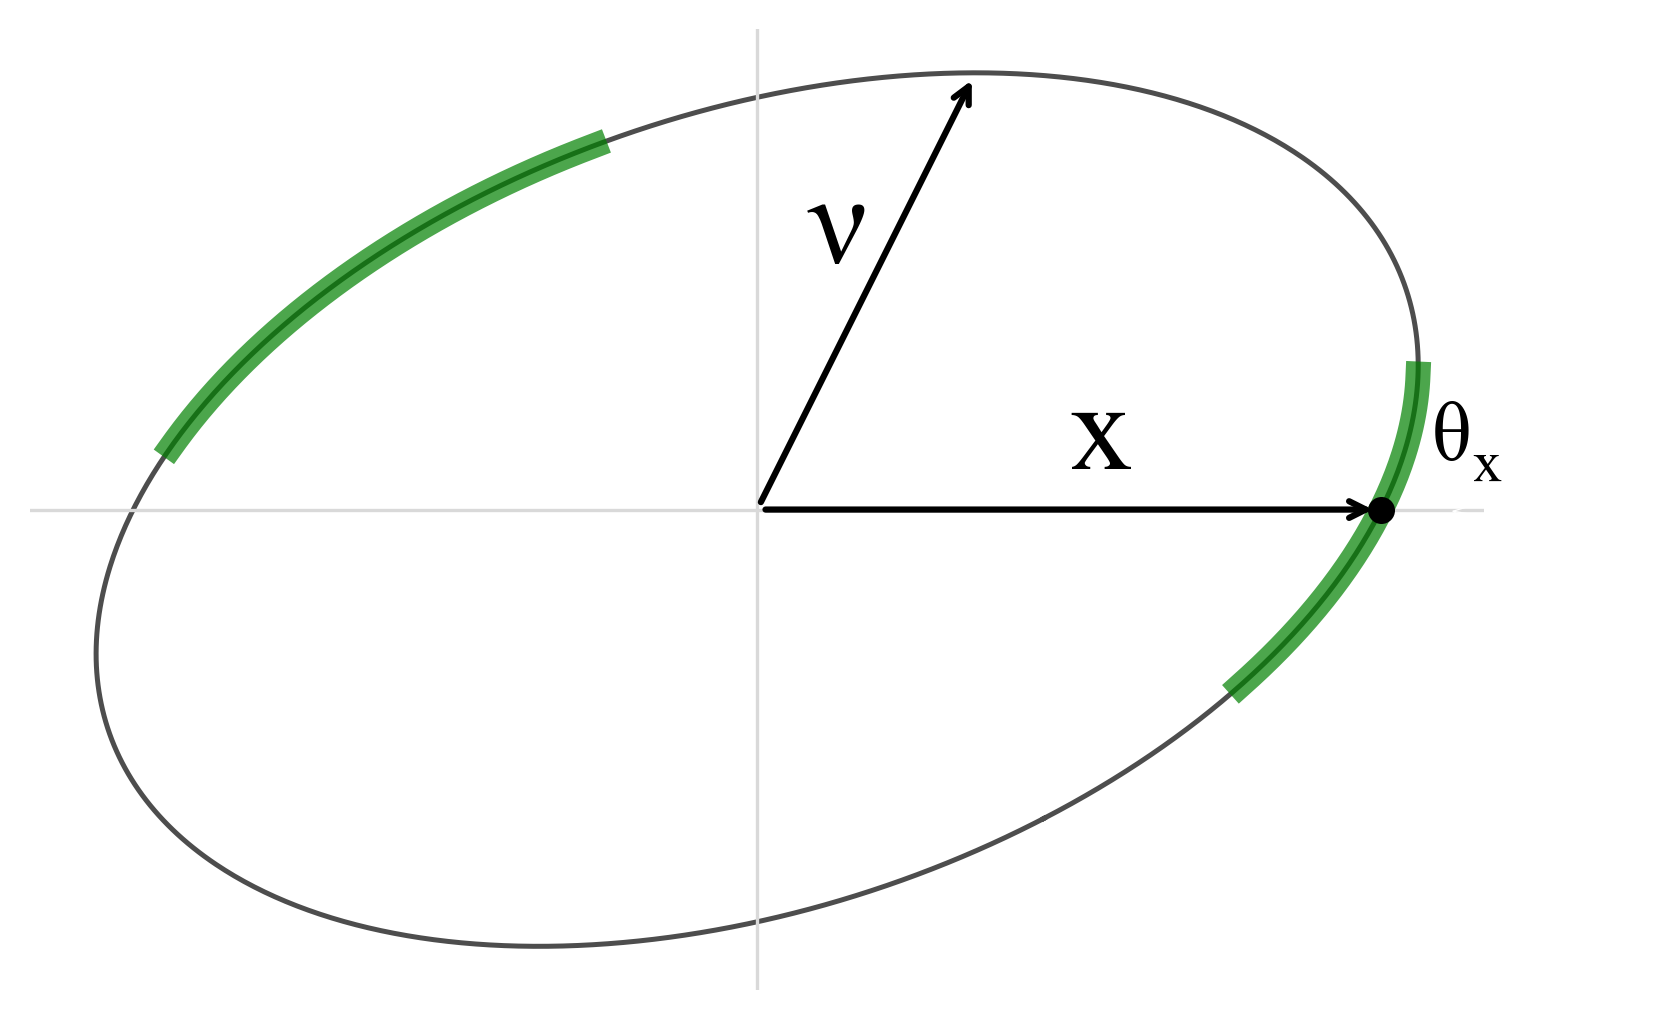
\includegraphics[width=0.7\linewidth]{ess_ellipse_one_proposal_nolabel.png}}
    \only<4>{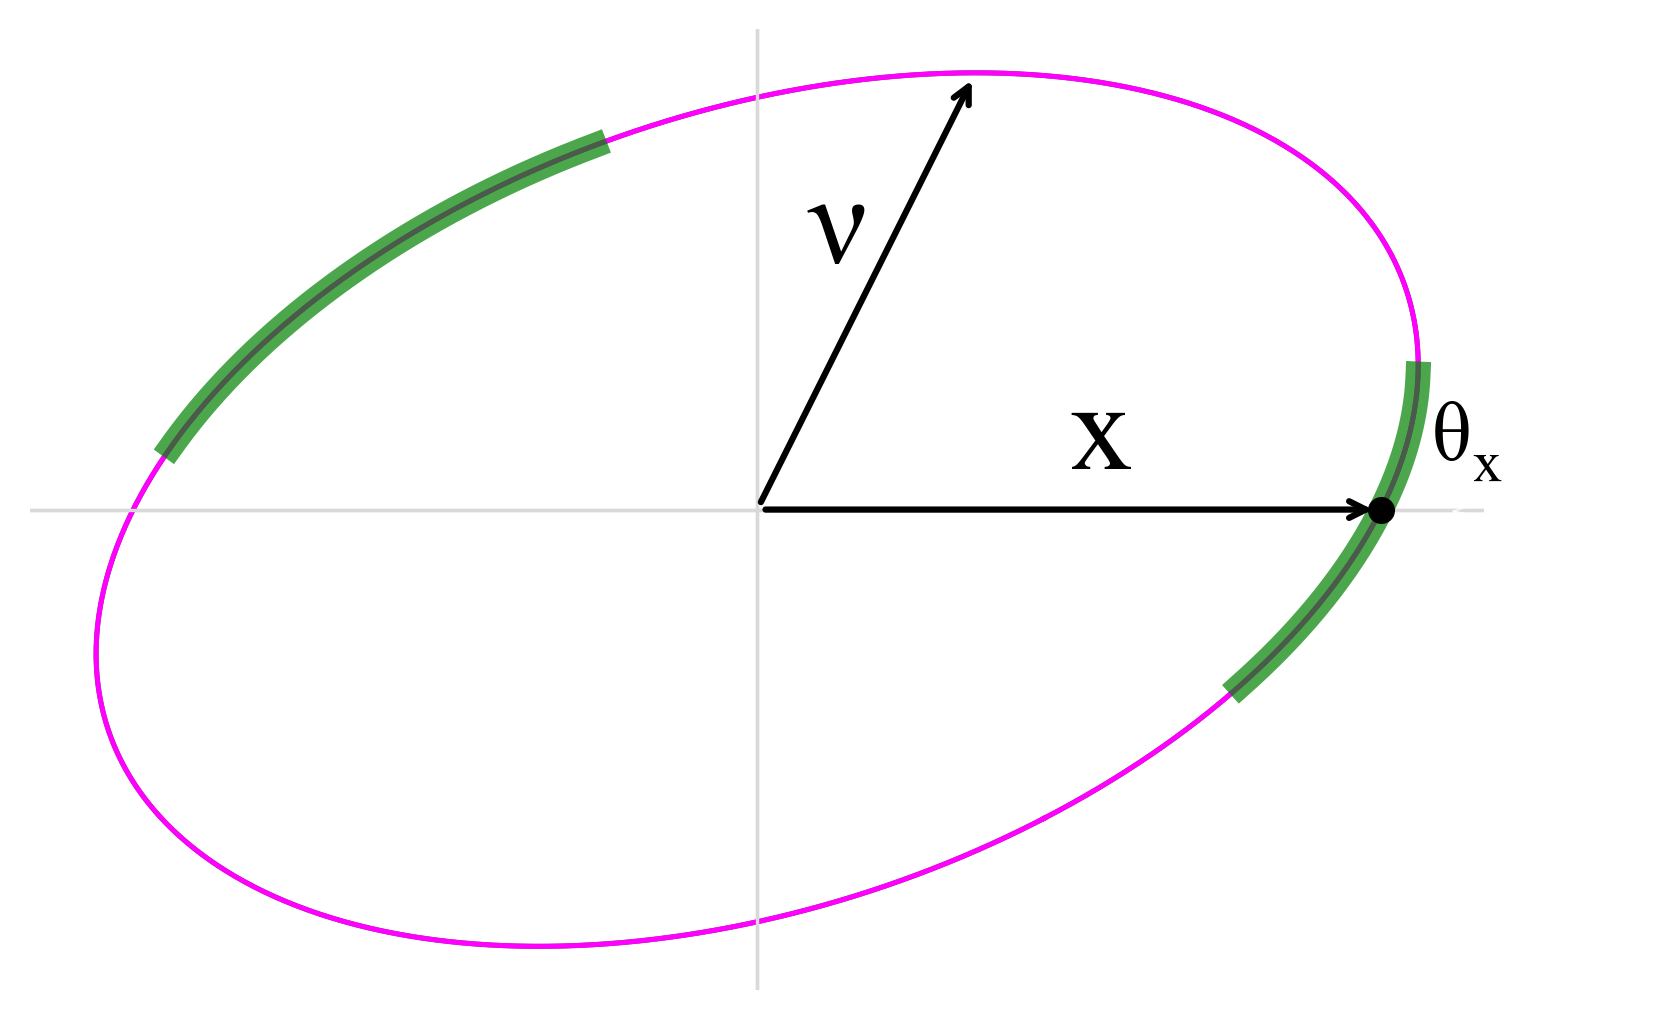
\includegraphics[width=0.7\linewidth]{ess_ellipse_one_proposal_pinkinterval.png}}
    \only<5>{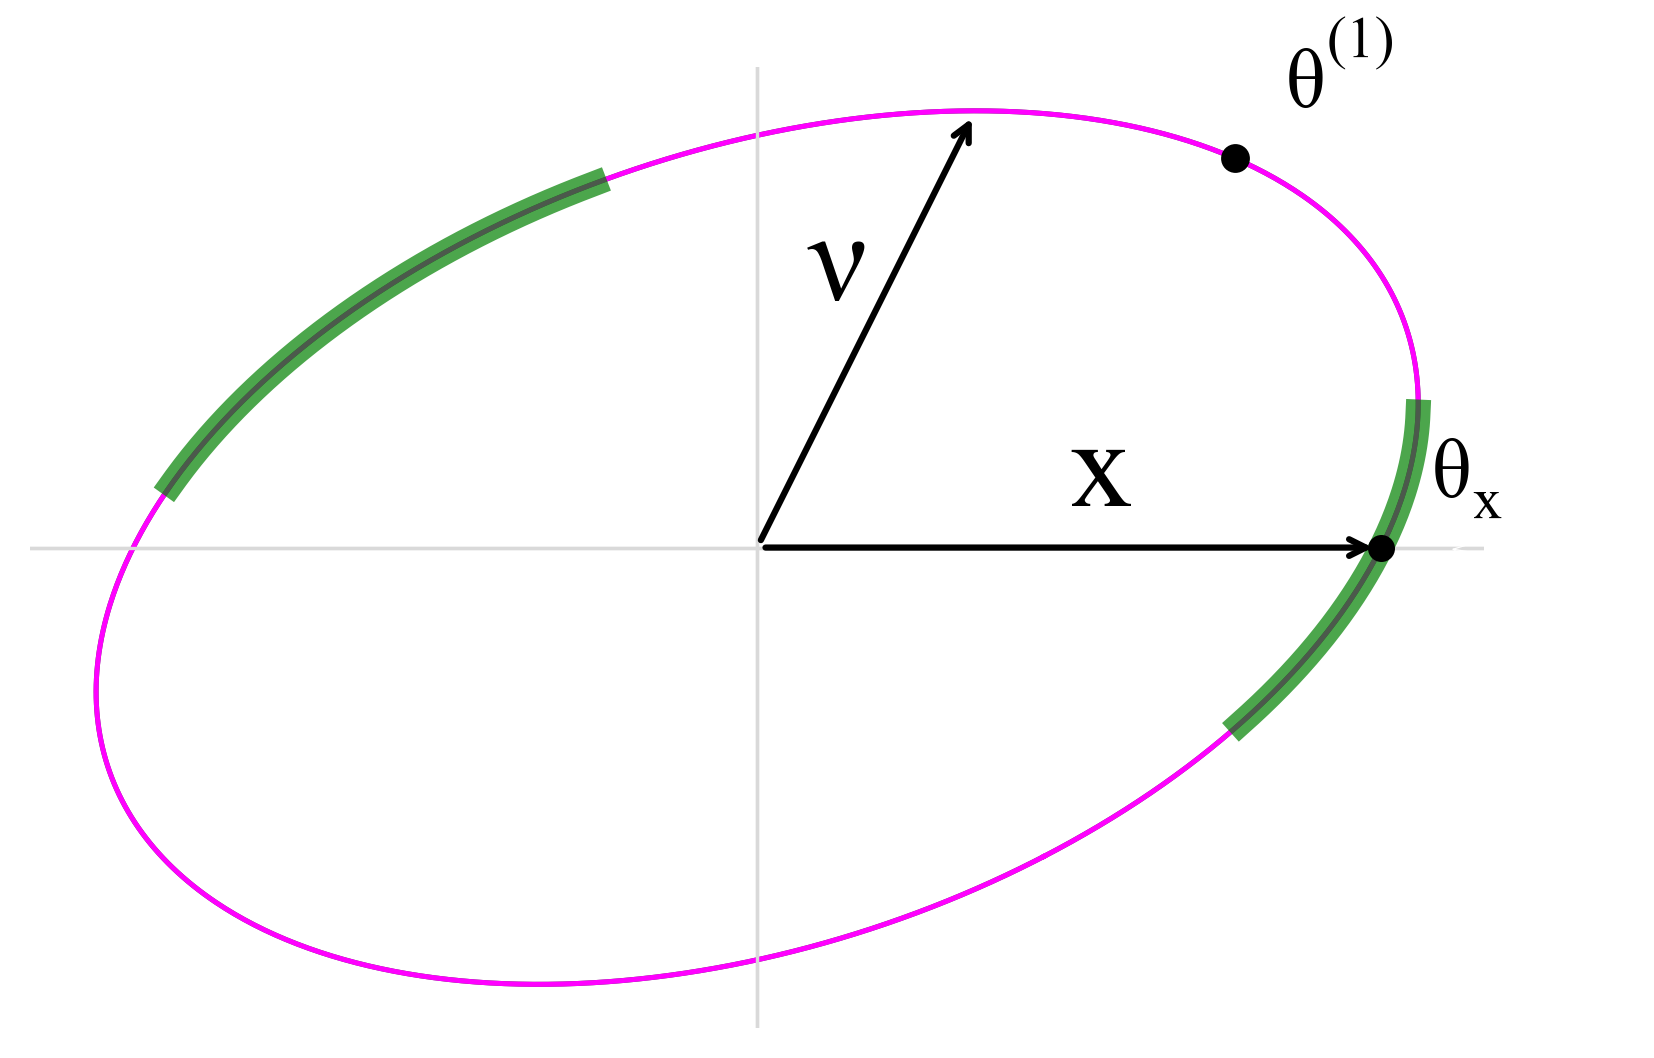
\includegraphics[width=0.7\linewidth]{ess_ellipse_one_proposal.png}}
    \end{figure}
\end{column}
\end{columns}
\end{frame}

\begin{frame}{One iteration of Elliptical Slice Sampling}
\begin{figure}
    \centering
    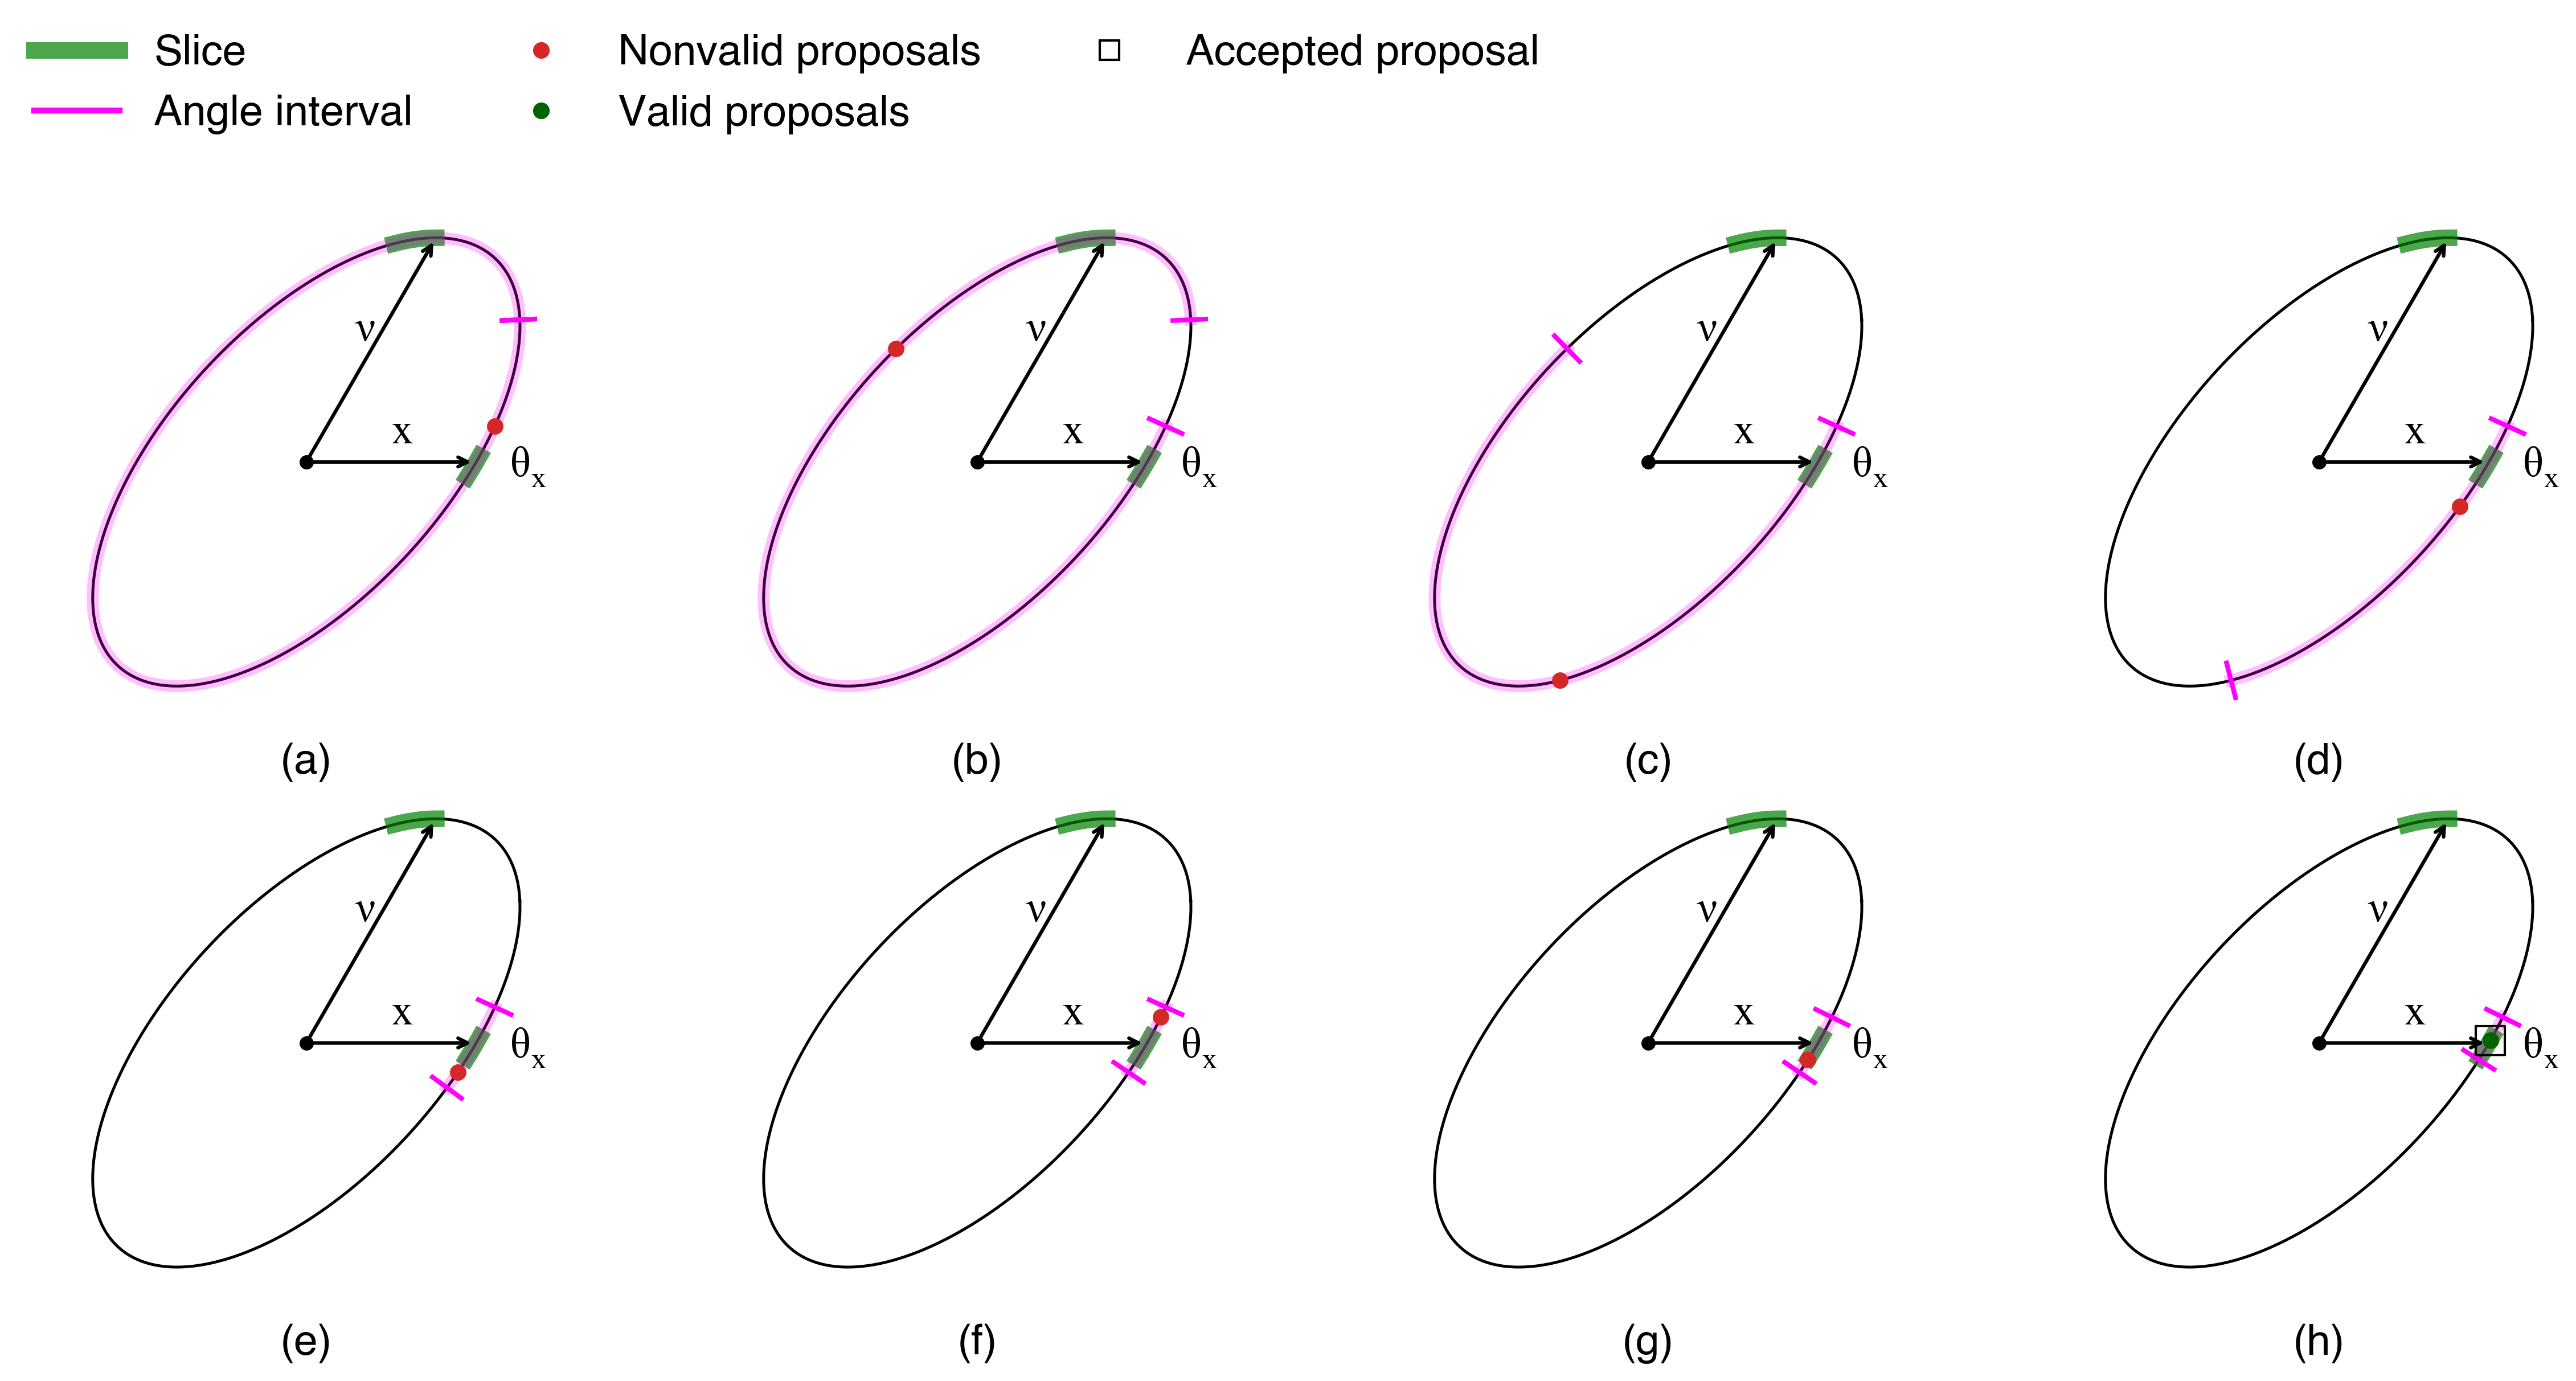
\includegraphics[width=0.7\linewidth]{mess_ellipses_iter_5007_M1.png}
    \caption{One iteration of ESS.}
\end{figure}
\end{frame}

% \begin{frame}{ESS algorithm (modified) \citet{Murray2010}}
% \begin{columns}[t]
% \begin{column}{0.45\textwidth}
% \begin{algorithm}[H]
% \caption{Elliptical Slice Sampler (modified) \citet{Murray2010}}
% \SetKwInOut{Input}{Input}
% \Input{Current state $\bm{x}$, prior draw $\bm{\nu}$, likelihood $\mathcal{L}(\bm{x})$.}
% \DontPrintSemicolon
% Sample $u \sim \mathcal{U}(0,1)$ and set $y \gets u\,\mathcal{L}(\bm{x})$\;
% Sample $\alpha \sim \mathcal{U}(0,2\pi]$ and set $\ell_0\!=0,\; r_0\!=2\pi$\;
% \For{$i=1,2,\ldots$}{
%     Sample $\varphi_i \sim \mathcal{U}(\ell_{i-1}, r_{i-1}]$\;
%     Propose $\tilde{\bm{x}}=\bm{x}\cos(\varphi_i-\alpha)+\bm{\nu}\sin(\varphi_i-\alpha)$\;
%     \If{$\mathcal{L}(\tilde{\bm{x}}) \ge y$}{Accept $\bm{x}\gets\tilde{\bm{x}}$ and return}\;
%     \Else{Shrink $(\ell_i,r_i)$ around $\alpha$}\;
% }
% \end{algorithm}
% \end{column}
% \begin{column}{0.55\textwidth}
% \vspace{0.2em}
% \begin{figure}
%     \centering
%     \begin{tikzpicture}[scale=0.95]
%         \draw[thick] (0,0) ellipse (2.1 and 1.2);
%         \draw[thick, dashed] (-1.5,0.6) arc (160:40:2.0 and 1.2);
%         \draw[thick, dashed] (-1.6,-0.5) arc (200:320:2.0 and 1.2);
%         \fill (1.2,0.2) circle (2pt) node[above right] {$x$};
%         \fill (-0.4,0.9) circle (2pt) node[above left] {$\nu$};
%         \node at (-0.2,1.35) {slice segments};
%         \draw[-{Stealth[length=2mm]}] (1.2,0.2) -- (0.2,0.95);
%         \node at (0.5,0.75) {$\theta$};
%     \end{tikzpicture}
%     \caption{ESS ellipse and slice (schematic).}
% \end{figure}
% \end{column}
% \end{columns}
% \end{frame}

% \begin{frame}{ESS geometry and pCN connection}
% \begin{itemize}
%     \item Ellipse defined by current state and prior draw; rotation preserves Gaussian prior.
%     \item pCN structure suggests dimension-robust behavior (Hilbert space setting).
%     \item This motivates MESS for large-scale Bayesian PDE inverse problems.
% \end{itemize}
% \end{frame}

% --------------------------------
\section{MESS}

\begin{frame}{Multiproposal Elliptical Slice Sampling}
\begin{columns}
\begin{column}{0.6\textwidth}
\begin{algorithm}[H]
\caption{MESS (single iteration)}
\SetKwInOut{Input}{Input}
\Input{Current state $x$, number of proposals $M$.}
\DontPrintSemicolon
% Draw $\nu\sim\mathcal{N}(0,C)$\;
% Draw $\theta_x \sim \mathcal{U}(0, 2\pi)$\;
% Draw slice level $y \sim \mathcal{U}(0, \mathcal{L}(\mathsf{y}|x))$\;
Draw $\nu\sim\mathcal{N}(0,C), \;\theta_x \sim \mathcal{U}(0, 2\pi), \;y \sim \mathcal{U}(0, \mathcal{L}(\mathsf{y}|x))$\;
Set $\theta_{\text{min}} \gets 0$, $\theta_{\text{max}} \gets 2\pi$\;
\While{$|\mathcal{A}|=0$}{
    Draw $\theta^{(j)} \sim \mathcal{U}(\theta_{\text{min}}, \theta_{\text{max}}), \quad j=1,\ldots,M$ {\scriptsize \textcolor{orange}{parallelizable}}\;
    Propose $x^{(j)}=x\cos\theta^{(j)}+\nu\sin\theta^{(j)}$ \;
    Compute $\mathcal{A}=\{j: \mathcal{L}(\mathsf{y}|x^{(j)})\ge y\}$\;
    Shrink using all angles
    %    \If{$|\mathcal{A}|=0$}{shrink using all $M$ angles and continue\;}
    % \Else{select $m\in\mathcal{A}$, set $x\leftarrow x^{(m)}$ and stop.\;}
}
Select $m\in\mathcal{A}$, set $x\leftarrow x^{(m)}$.\;
    % \Indp
% Draw $\bm{\theta}^{(1)}=(\theta^{(1)},\ldots,\theta^{(M)})$ in the bracket; propose $x^{(m)}=x\cos\theta^{(m)}+\nu\sin\theta^{(m)}$\;
% Compute $\mathcal{A}=\{m: \mathcal{L}(\mathsf{y}|x^{(m)})\ge y\}$\;
% \If{$|\mathcal{A}|=0$}{shrink the bracket using all $M$ angles and continue\;}
% \Else{select index $m\in\mathcal{A}$ (via transition matrix), set $x\leftarrow x^{(m)}$, stop\;}
% \Indm
\end{algorithm}
\vspace{0.25em}
\end{column}
\begin{column}{0.4\textwidth}
% \begin{figure}
% \centering
% 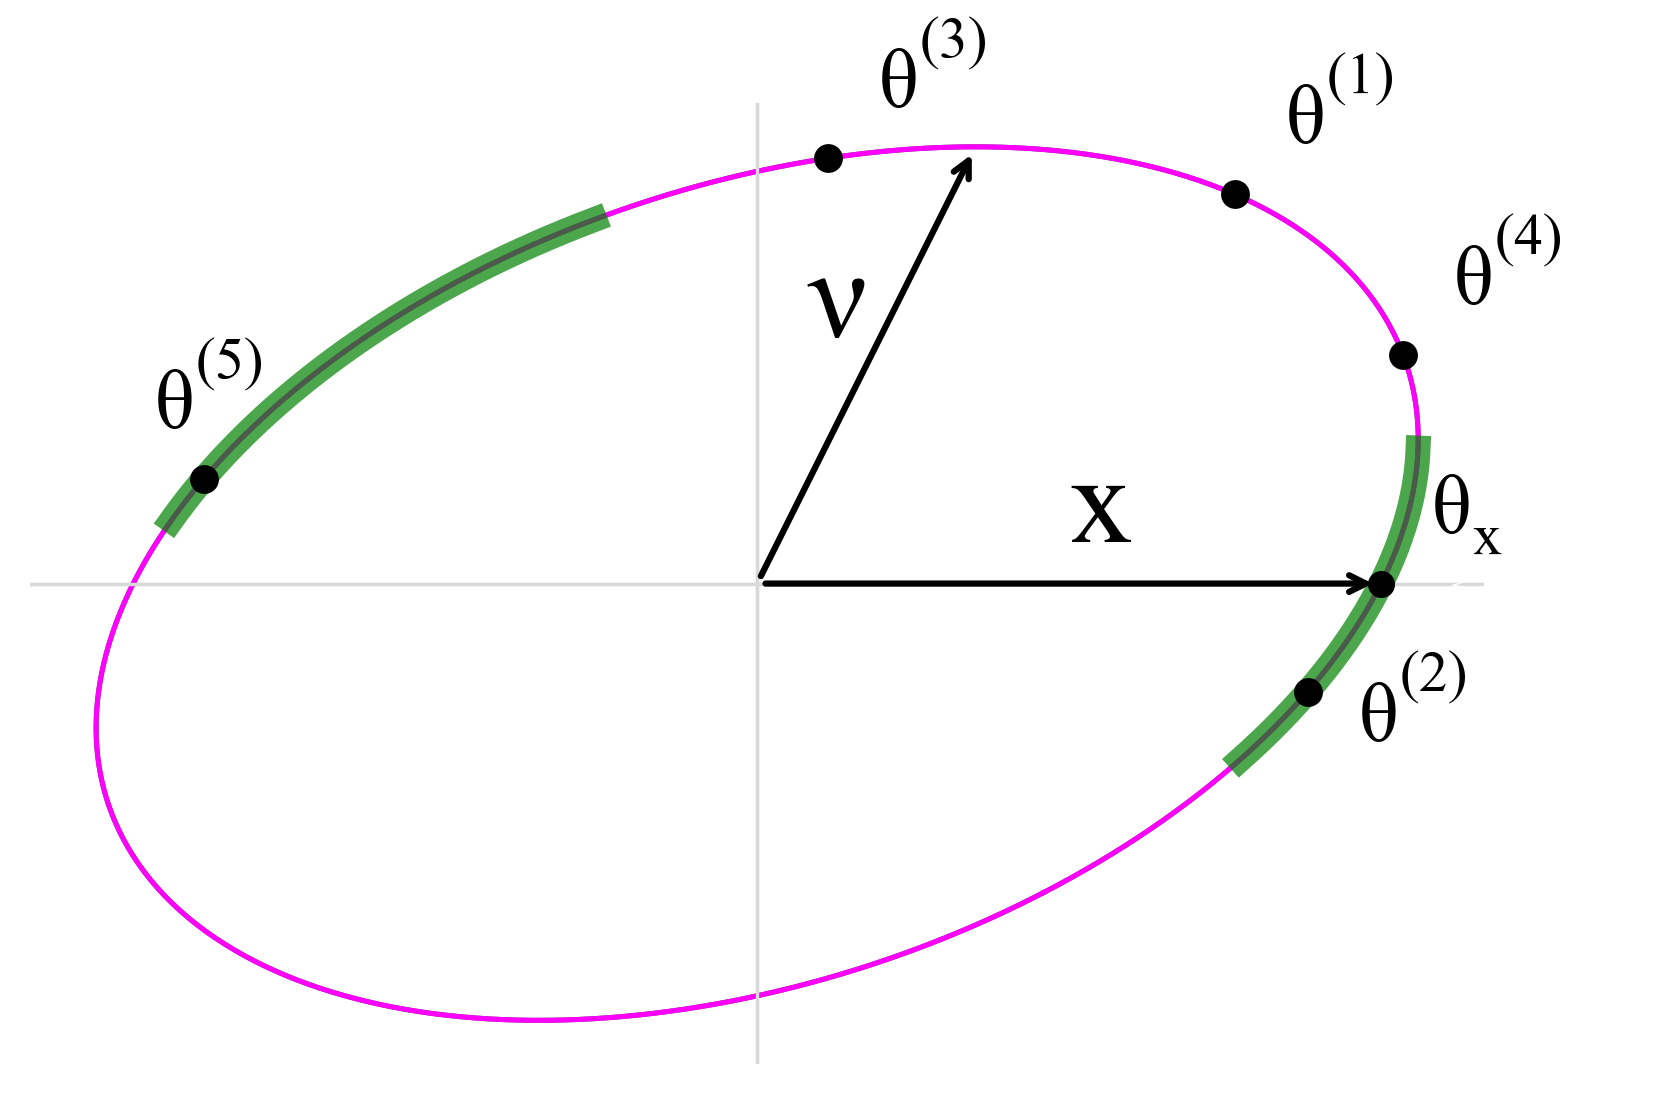
\includegraphics[width=0.8\linewidth]{mess_ellipse_5_proposals.png}
% \caption{MESS ($M=5$).}
% \end{figure}
    \begin{figure}
    \centering
    \only<1>{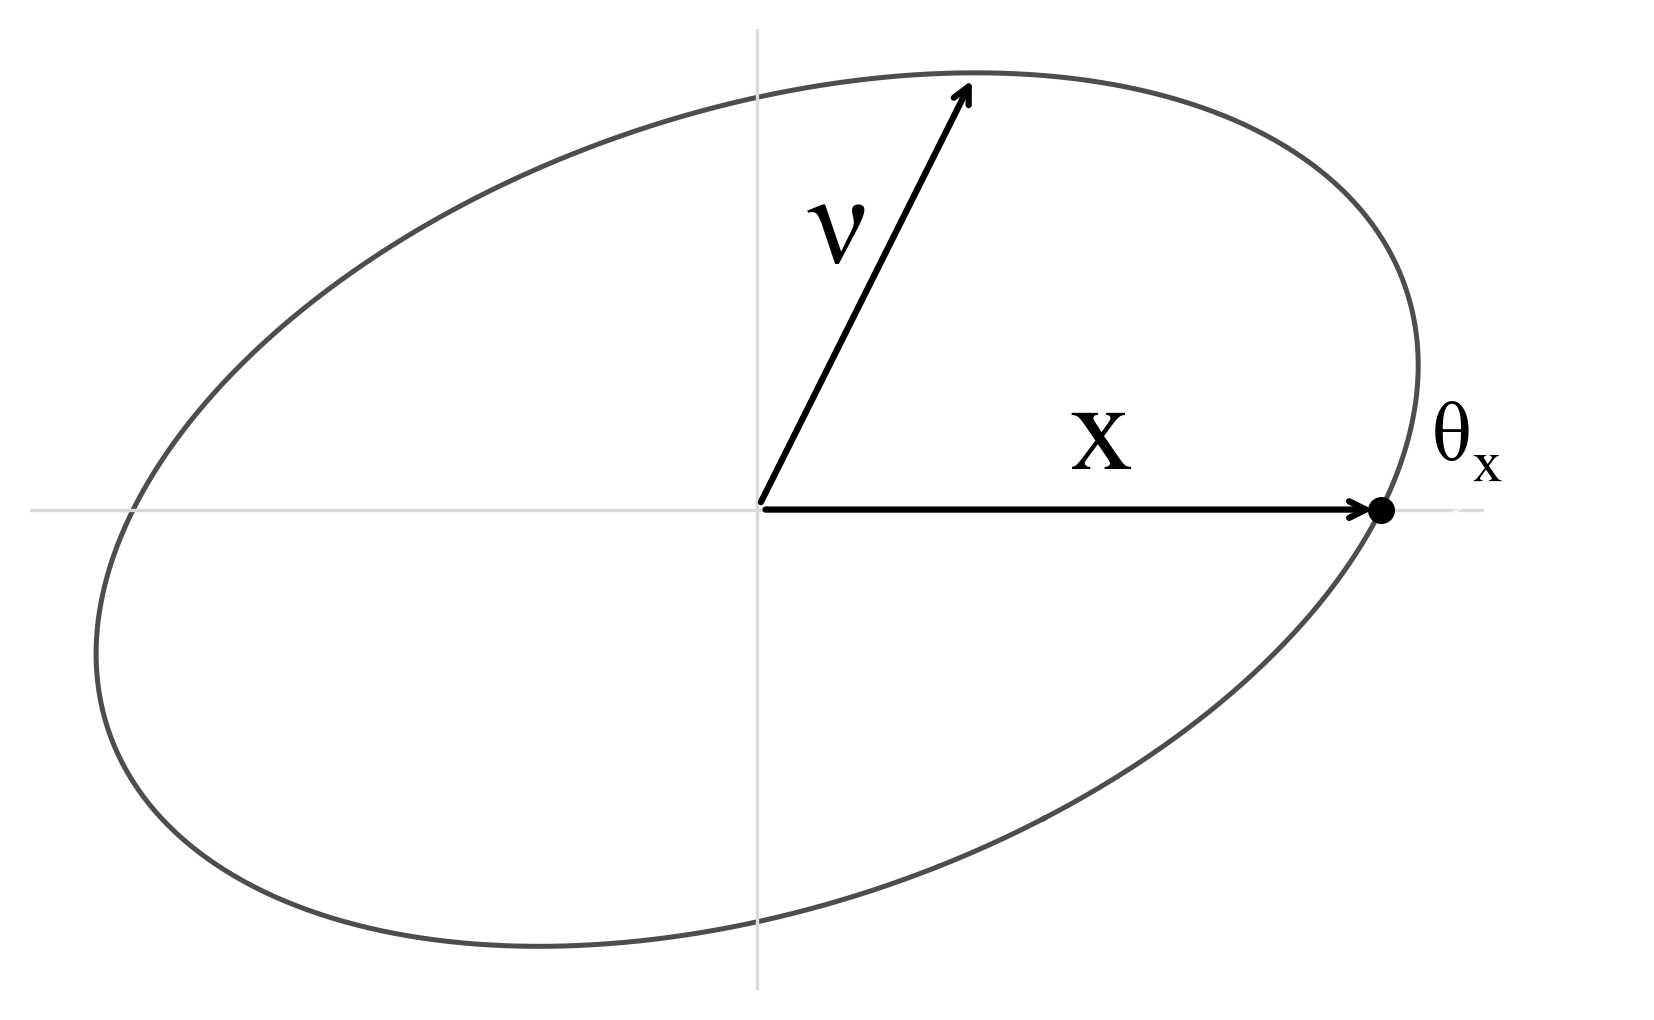
\includegraphics[width=0.7\linewidth]{ess_ellipse_one_proposal_nolabel_noslice.png}}
    \only<2>{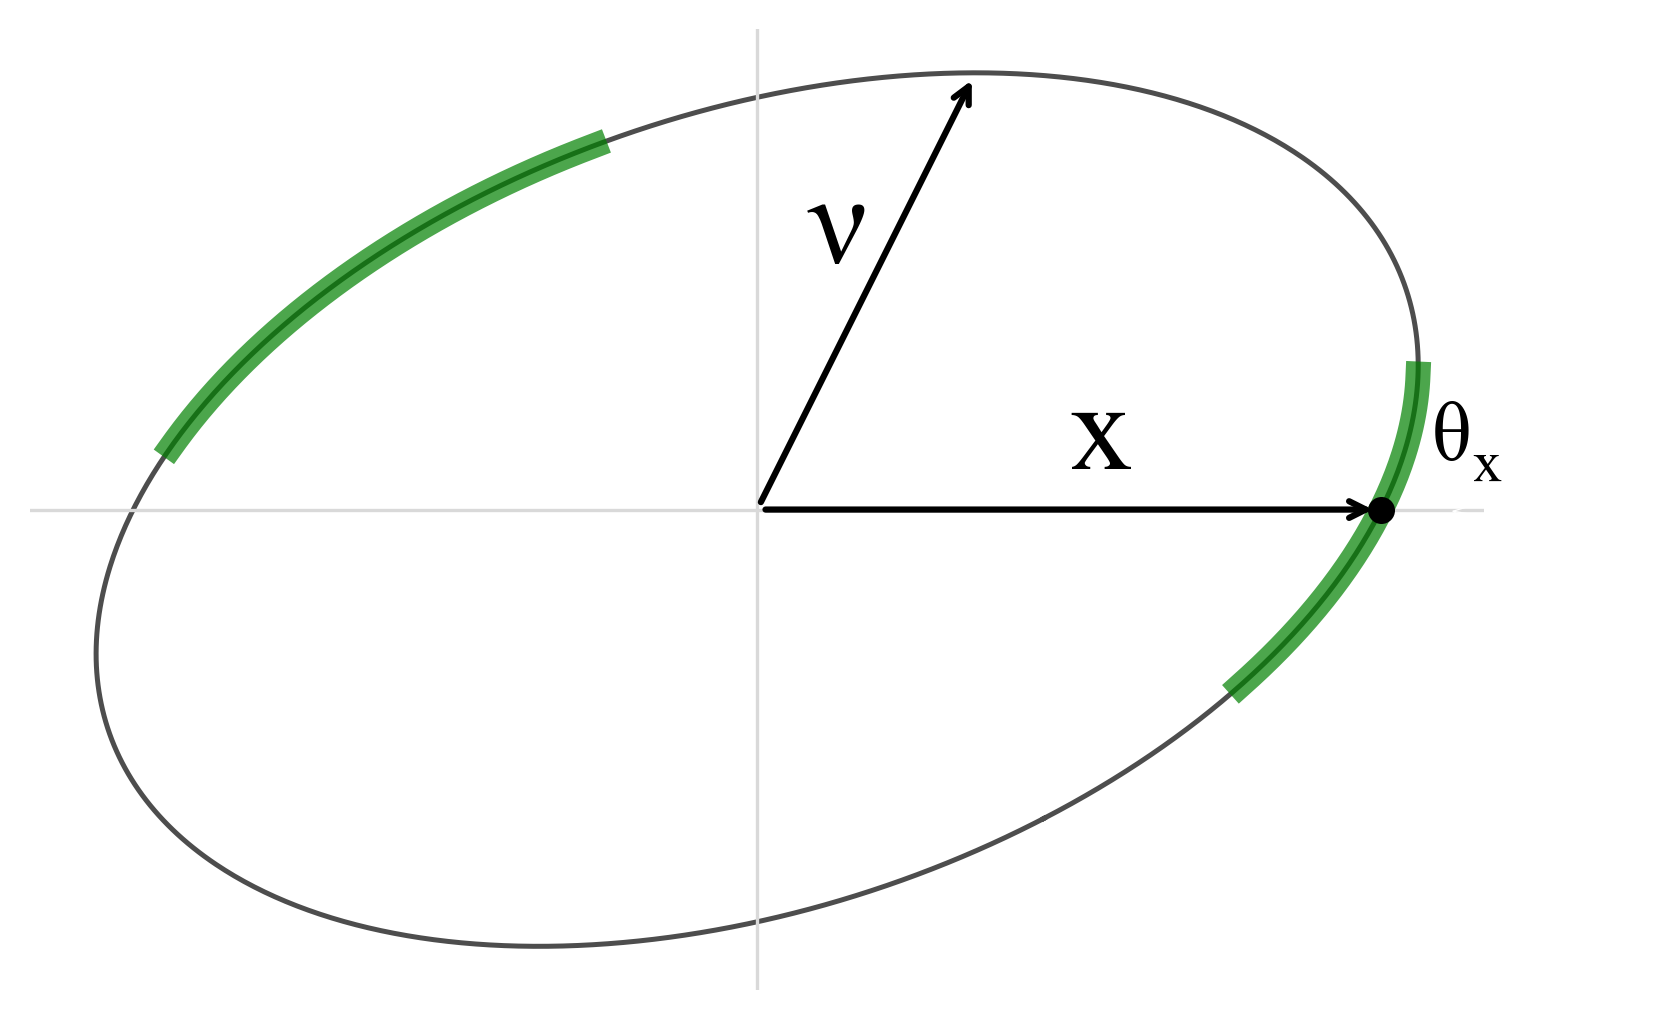
\includegraphics[width=0.7\linewidth]{ess_ellipse_one_proposal_nolabel.png}}
    \only<3>{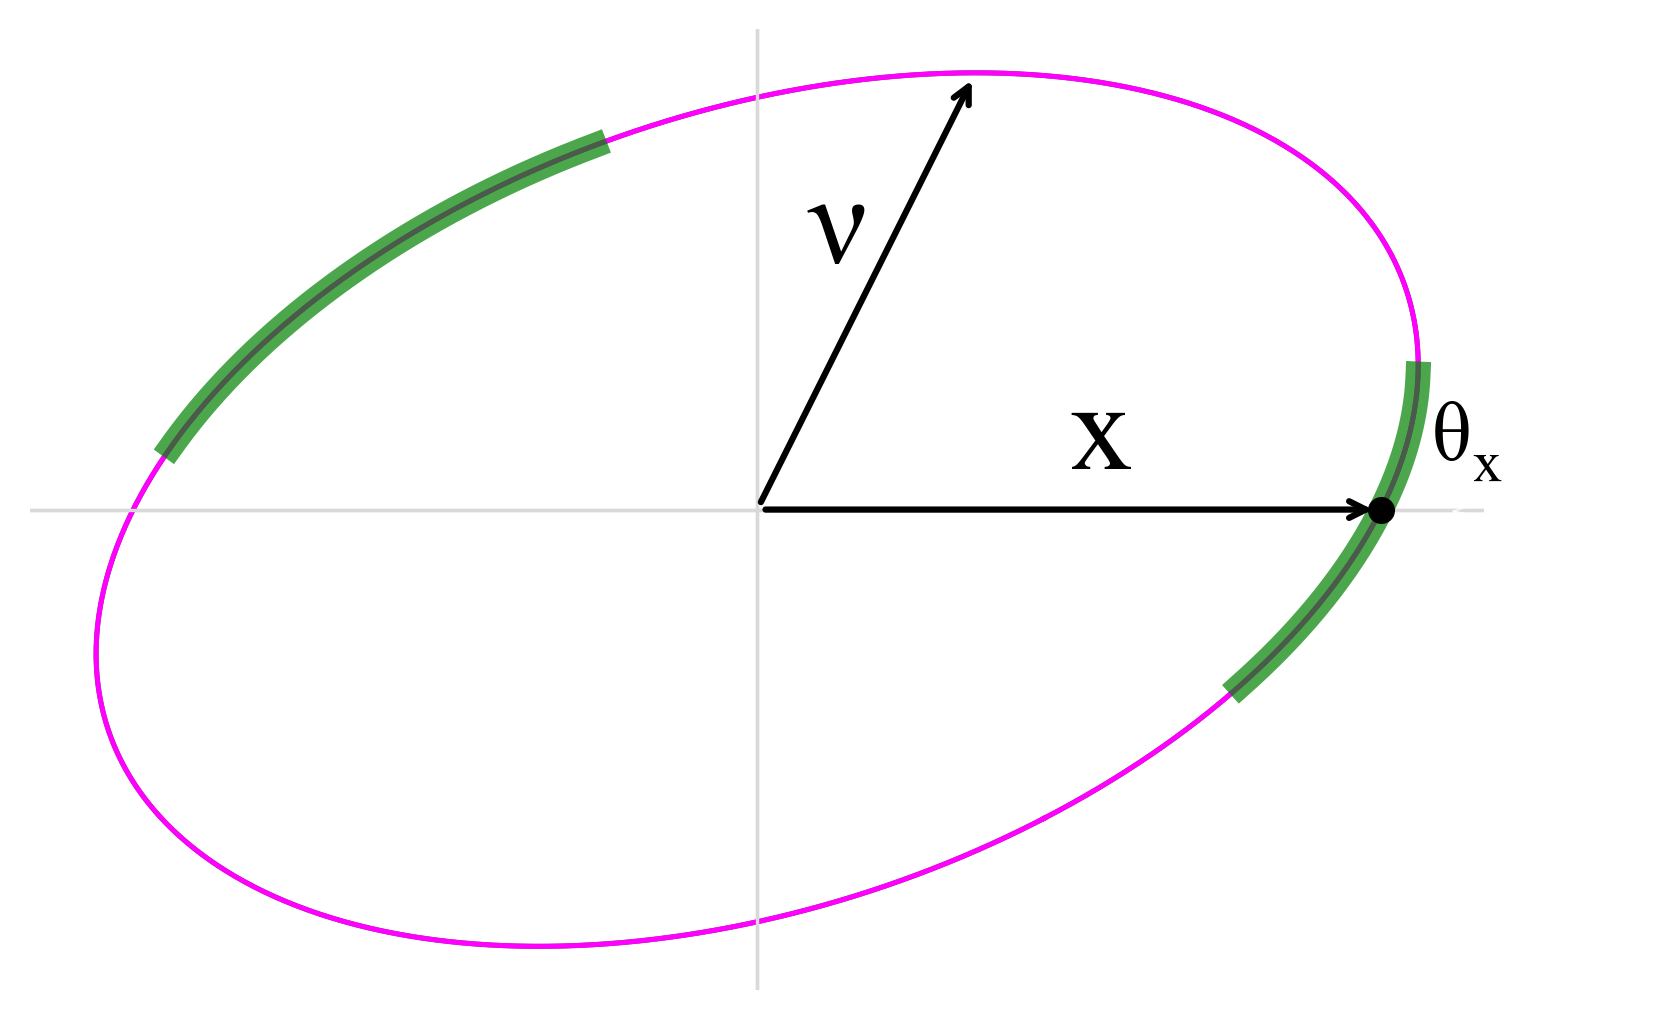
\includegraphics[width=0.7\linewidth]{ess_ellipse_one_proposal_pinkinterval.png}}
    \only<4>{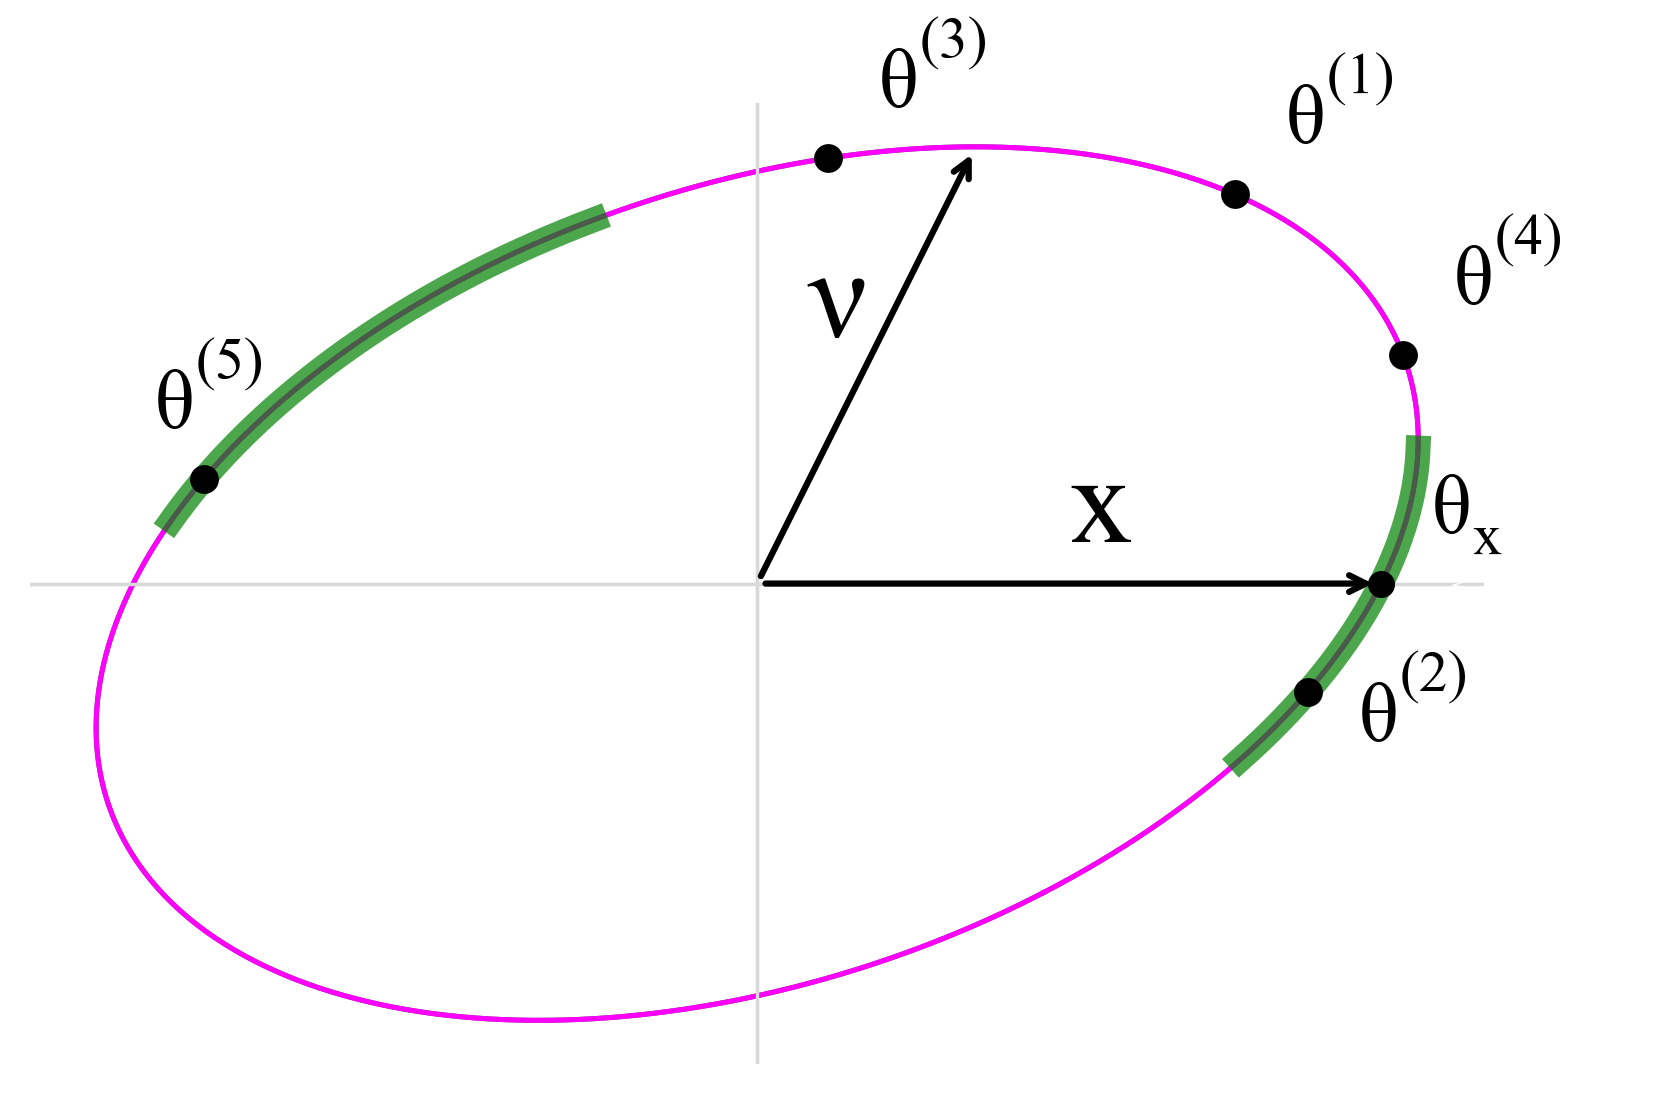
\includegraphics[width=0.7\linewidth]{mess_ellipse_5_proposals.png}}
    \caption{MESS ($M=5$).}
    \end{figure}
\end{column}
\end{columns}
\end{frame}

\begin{frame}{Mess in action}
\begin{figure}
    \centering
    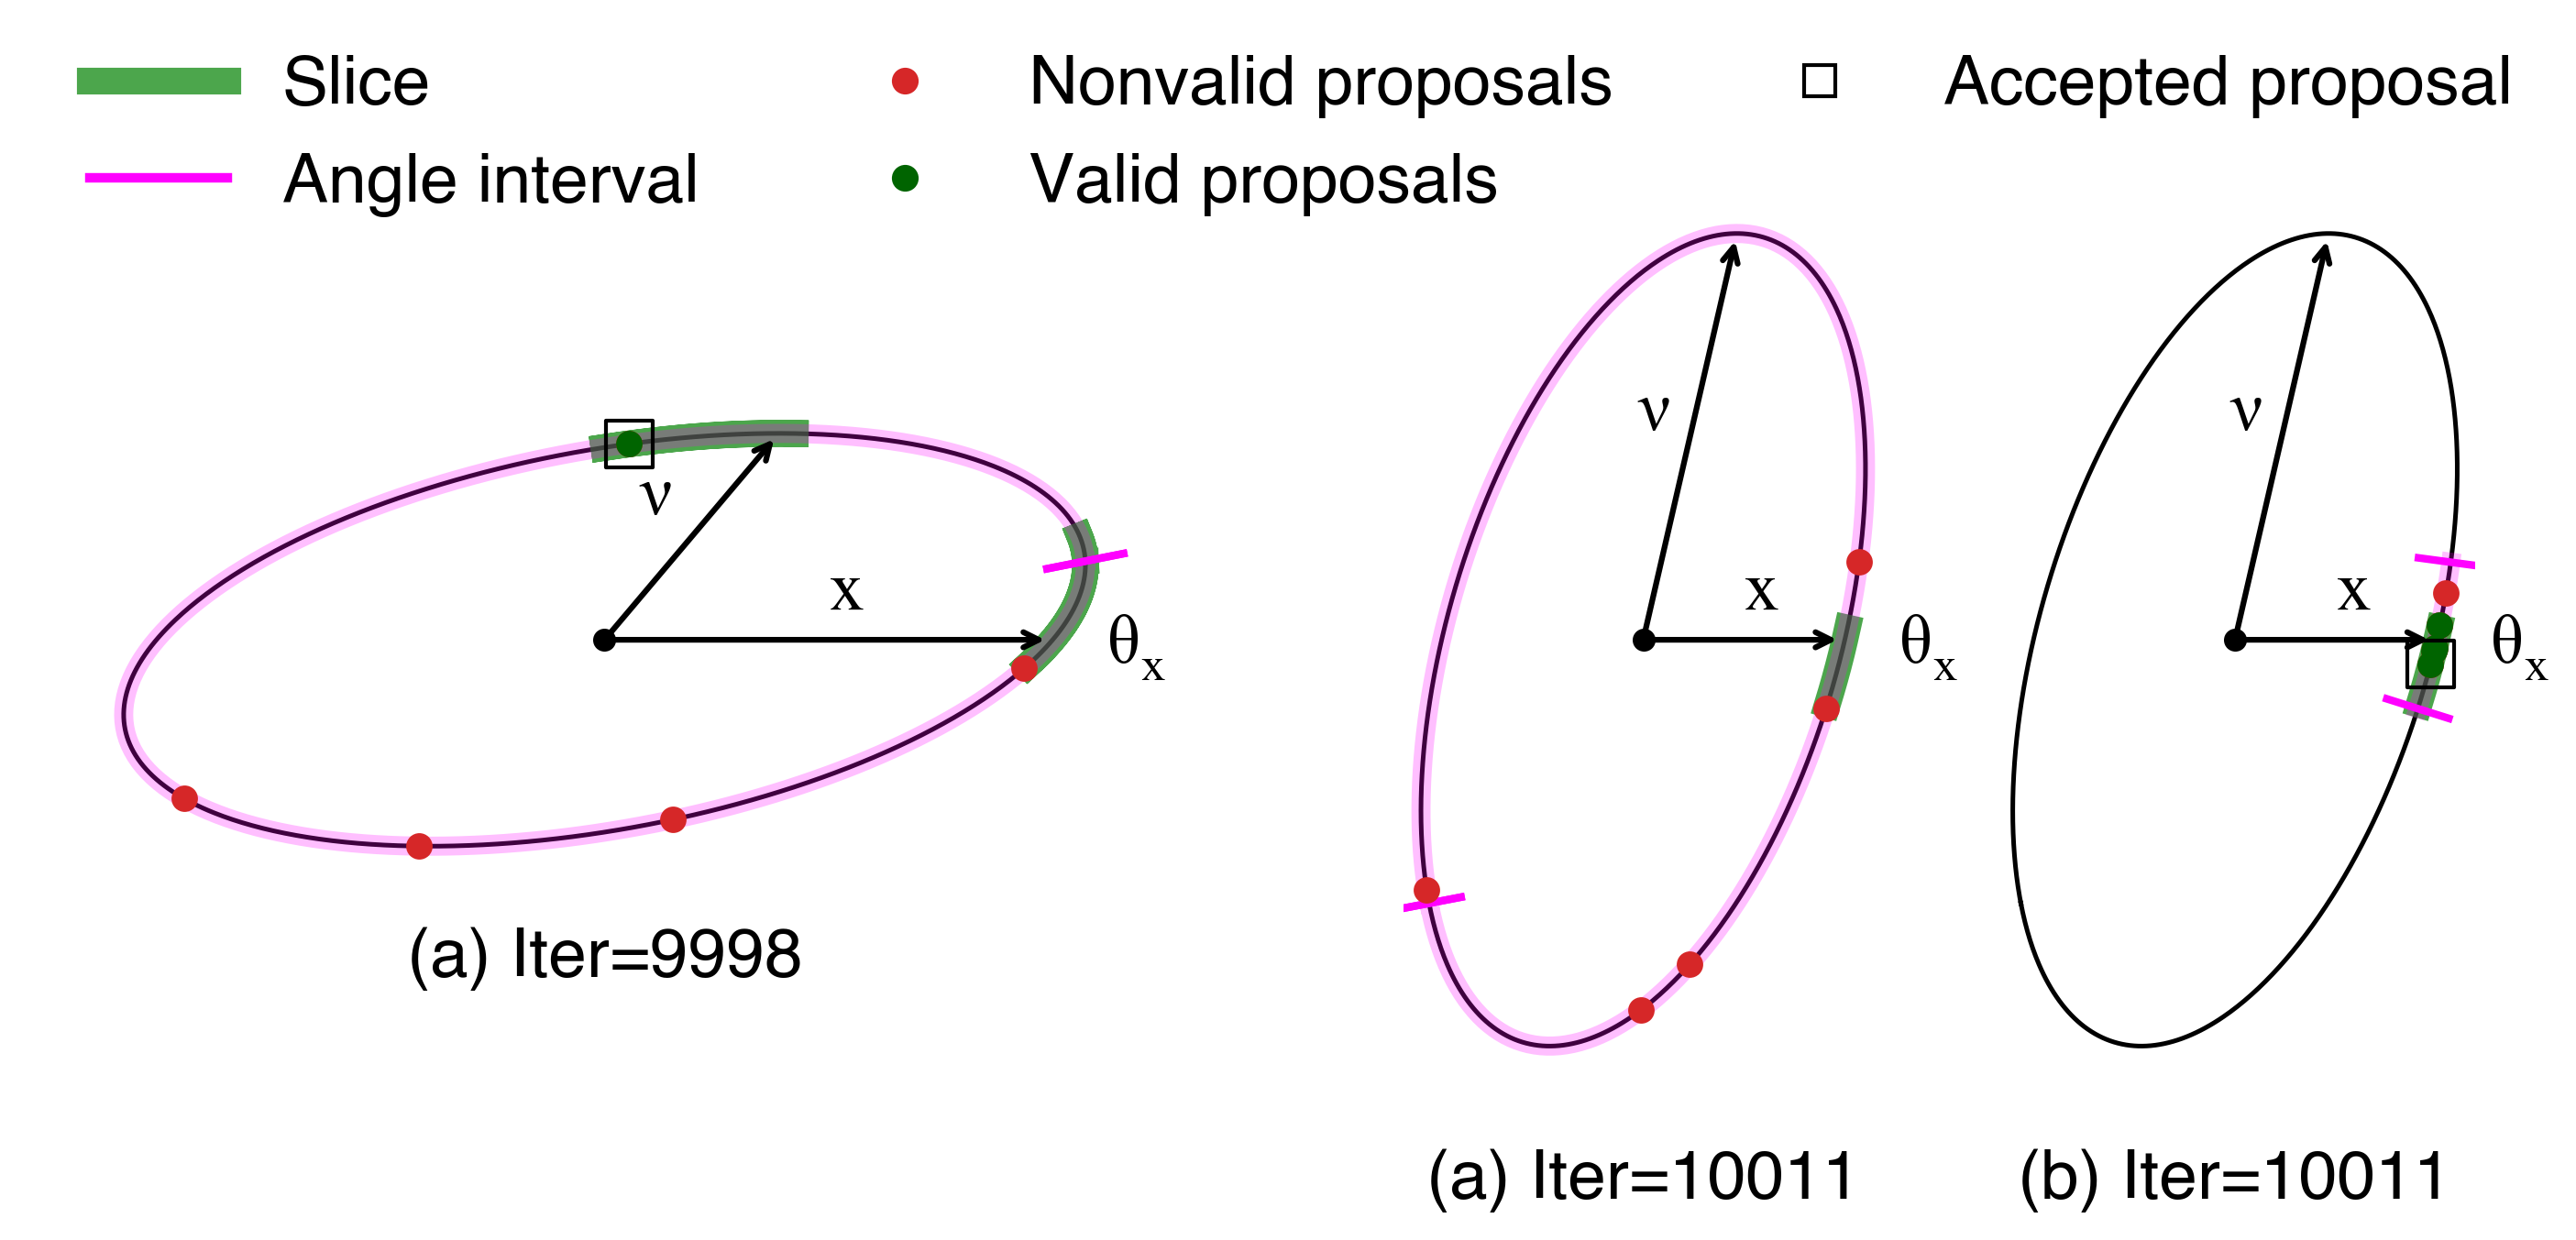
\includegraphics[width=0.7\linewidth]{mess_ellipses_iters_9998_10011.png}
    \caption{Two iterations of MESS with $M=5$.}
\end{figure}
\end{frame}

% \begin{frame}{Multiproposal Elliptical Slice Sampling}
% \begin{itemize}[<+->]
%     \item Draw $M$ angles in parallel: 
%     \[ \bm{\varphi}_i=(\varphi_{i1},\ldots,\varphi_{iM}). \]
%     \vspace{0.25em}
%     \item Evaluate their likelihoods in parallel:

%     \[ \{\mathcal{L}(x^{(j)}) , \quad j=1, \ldots, M\} \]
%     \vspace{0.25em}
%     \item Check if they are valid (i.e., if they hit the slice):
%     \[
%         \mathcal{A}_i = \{j: \mathcal{L}(\tilde{x}^{(j)}) \ge y\}.
%     \]
%     \vspace{0.25em}
%     \item If $|\mathcal{A}_i|=0$, shrink using all $M$ angles.
%     \vspace{0.25em}
%     \item Else, choose $j$ from $\mathcal{A}_i$ with probabilities defined by a Markov transition matrix. 
% \end{itemize}
% \end{frame}

% \begin{frame}{Acceptance step with transition matrix}
% \begin{columns}[t]
% \begin{column}{0.55\textwidth}
% \begin{itemize}[<+->]
%     \item At iteration $k$:$\quad \bm{\varphi}_k = \{\varphi_{k1}, \ldots, \varphi_{k5} \}$
%     \item Two angles are valid: $\quad \mathcal{A}_k=\{2, 4\}$.
%     \item Unordered vector of valid angles: 
%     \[
%     \bm{\psi}=(\alpha, \varphi_{k2},\varphi_{k4})
%     \]
%     \item Ordered vector: 
%     \[
%     \bm{\psi}^{\uparrow}=(\varphi_{k2}, \alpha, \varphi_{k4})
%     \]
%     \item Transition matrix:
%     \[
%     \bm{P}=\begin{bmatrix}
%     0 & P_{12} & P_{13}\\
%     P_{21} & 0 & P_{2B}\\
%     P_{31} & P_{32} & 0
%     \end{bmatrix}
%     \]
% \end{itemize}
% \end{column}
% \begin{column}{0.45\textwidth}
%     \begin{figure}
%     \begin{subfigure}[t]{0.6\textwidth}
%         \centering
%         \includegraphics[width=\linewidth]{/Users/guillers/Documents/GitHub/mess-internal/reports/presentations/iscam_march_2026/images/acceptance_step_chronological_M5.png}
%     \end{subfigure}
%     \vspace{0.4em}
%     \begin{subfigure}[t]{0.6\textwidth}
%         \centering
%         \includegraphics[width=\linewidth]{/Users/guillers/Documents/GitHub/mess-internal/reports/presentations/iscam_march_2026/images/acceptance_step_ordered_M5.png}
%     \end{subfigure}
%     \end{figure}
% \end{column}
% \end{columns}
% \end{frame}

\begin{frame}{Acceptance step with transition matrix}
\begin{columns}[t]
\begin{column}{0.5\textwidth}
    % At subiteration $k$:
    \begin{itemize}
        \item<1-> Sample $\theta^{(1)},\ldots,\theta^{(5)}$.
        \item<2-> Valid indices: $\mathcal{A}:=\{j: \mathcal{L}(x^{(j)})\ge y\}=\{2,5\}$.
        % \item<3-> \textcolor{red}{Ordered} valid angles: 
        % \[
        %     (\theta^{(2)},\theta_x,\theta^{(5)}) \mbox{ with labels } (\textcolor{red}{0, 1, 2}).
        % \] 
        \item<4-> Transition matrix with entries 
        \[
        \bm{P}=\begin{bmatrix}
        P_{\textcolor{red}{22}} & P_{\textcolor{red}{2x}} & P_{\textcolor{red}{25}}\\
        P_{\textcolor{red}{x2}} & P_{\textcolor{red}{xx}} & P_{\textcolor{red}{x5}}\\
        P_{\textcolor{red}{52}} & P_{\textcolor{red}{5x}} & P_{\textcolor{red}{55}}
        \end{bmatrix}
        \]
        \item<5-> Naive choice (uniform):
        \[
        \bm{P}^{\text{unif}} =
        \begin{bmatrix}
        0 & 0.5 & 0.5 \\0.5 & 0 & 0.5 \\0.5 & 0.5 & 0
        \end{bmatrix}
        \]
    \end{itemize}
\end{column}
\begin{column}{0.5\textwidth}
    \vspace{-0.3cm}
    \begin{figure}
        \centering
        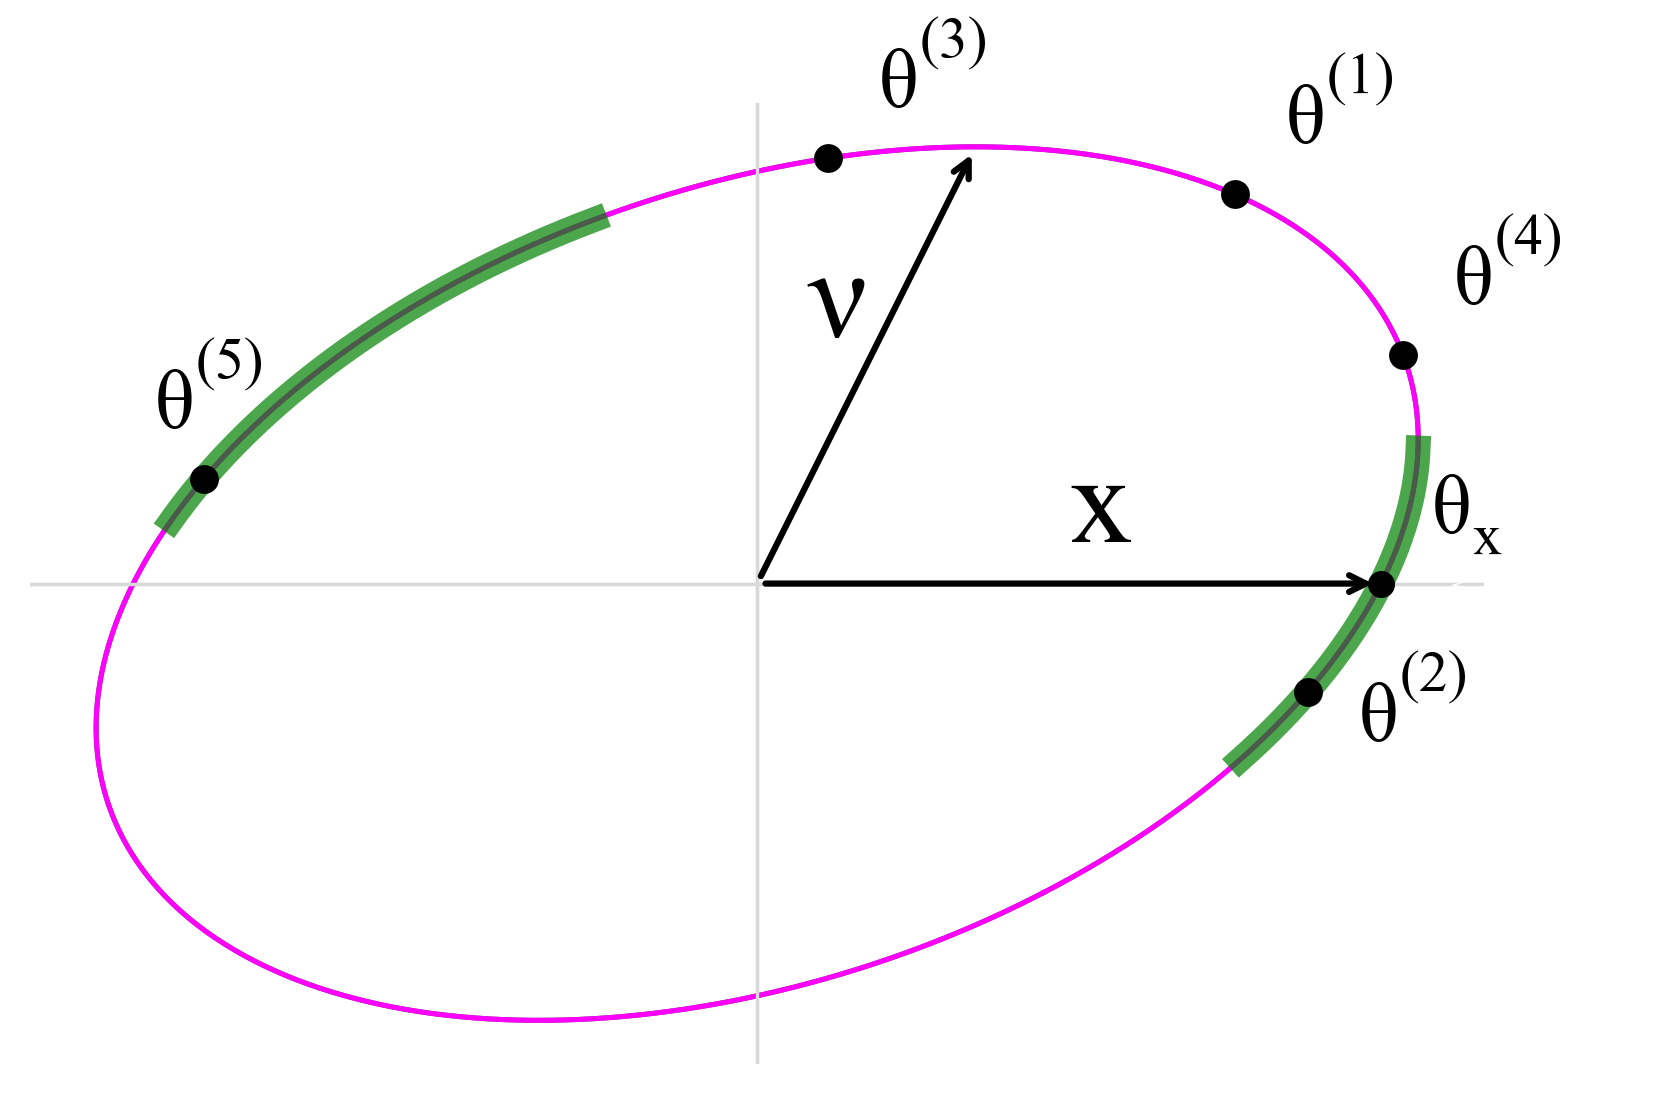
\includegraphics[width=0.8\linewidth]{mess_ellipse_5_proposals.png}
    \end{figure}
    %     \begin{figure}
    % \only<1-3>{
    %     \begin{subfigure}[t]{0.7\textwidth}
    %         \centering
    %         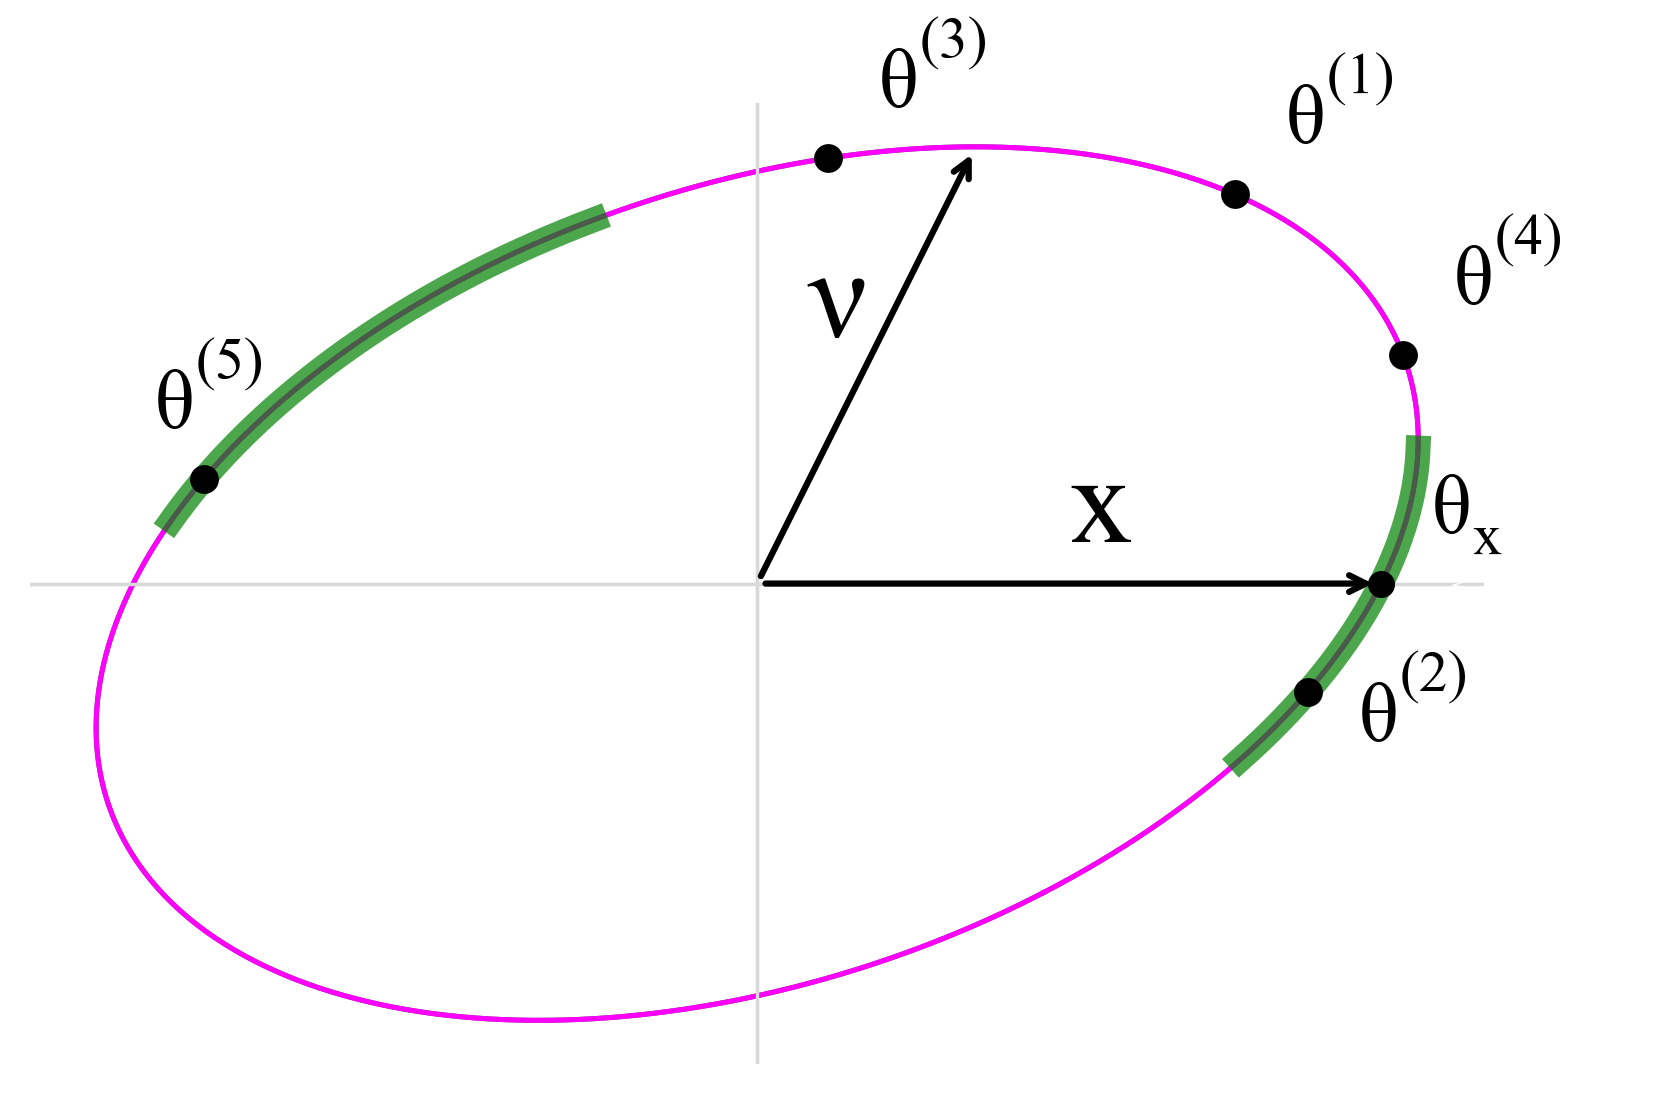
\includegraphics[width=\linewidth]{mess_ellipse_5_proposals.png}
    %     \end{subfigure}
    % }
    % \only<3->{
    %     \begin{subfigure}[t]{1\textwidth}
    %         \centering
    %         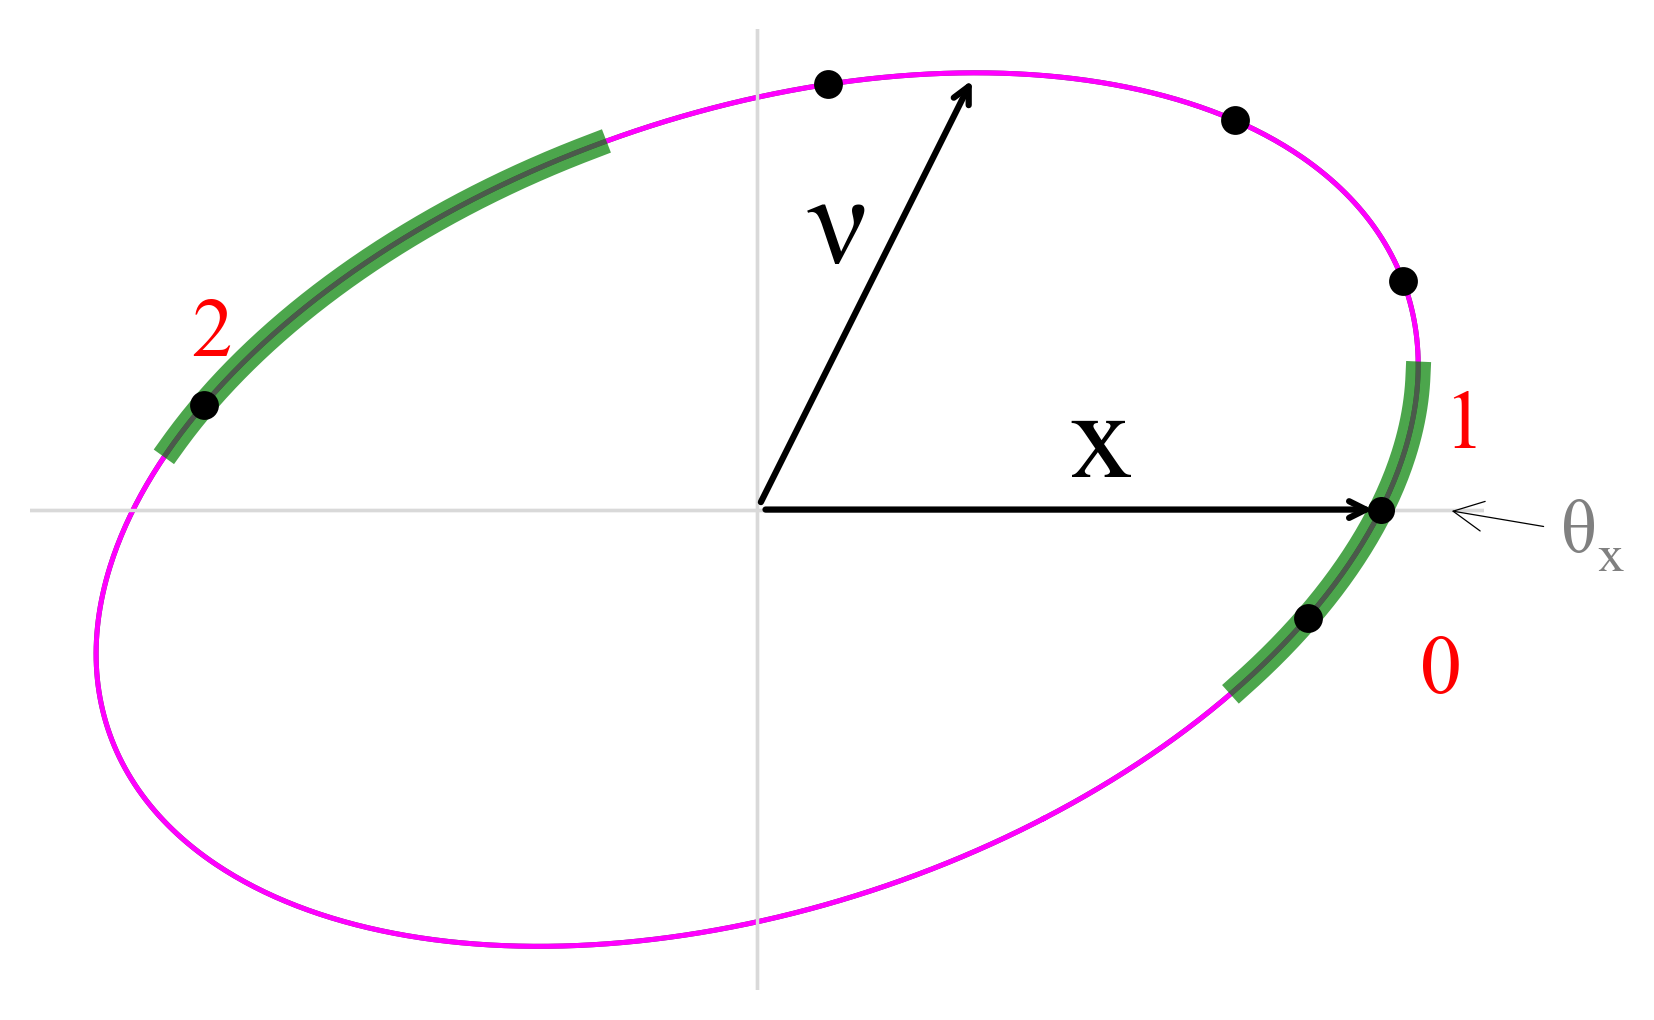
\includegraphics[width=0.7\linewidth]{mess_acceptance_redlabels_valid.png}
    %     \end{subfigure}
    % }
    % \end{figure}
    % \begin{itemize}
        % \item<4-> Unordered valid angles:
        % \[
        %     (\theta_x, \theta_{k}^{(2)},\theta_{k}^{(5)})
        % \]
        % \item<5-> \textcolor{red}{Ordered} valid angles: 
        % \[
        %     (\theta^{(2)},\theta_x,\theta^{(5)}) \mbox{ with labels } \textcolor{red}{(0, 1, 2)}.
        % \]
        % with labels \textcolor{red}{$(0, 1, 5)$}.
        % \item<6-> Transition matrix with entries 
        % \[
        % \bm{P}=\begin{bmatrix}
        % 0 & P_{\textcolor{red}{01}} & P_{\textcolor{red}{02}}\\
        % P_{\textcolor{red}{10}} & 0 & P_{\textcolor{red}{12}}\\
        % P_{\textcolor{red}{20}} & P_{\textcolor{red}{21}} & 0
        % \end{bmatrix}
        % \]
    % \end{itemize}
    % \begin{tikzpicture}[overlay,remember picture]
    %     \only<5->{\draw[red,rounded corners,thick]
    %         ($(pic cs:row2start)+(-0.6em,1.1ex)$) rectangle
    %         ($(pic cs:row2end)+(0.6em,-1.1ex)$);}
    % \end{tikzpicture}
\end{column}
\end{columns}
\end{frame}

\begin{frame}{Distance-informed transition matrix}
\begin{columns}[t]
\begin{column}{0.52\textwidth}
\begin{itemize}[<+->]
    % \item Naive choice (uniform):
    % \[
    % \bm{P}^{\text{unif}} =
    % \begin{bmatrix}
    % 0 & 0.5 & 0.5 \\0.5 & 0 & 0.5 \\0.5 & 0.5 & 0
    % \end{bmatrix}
    % \]
    \item Use distance to bias transitions:
    \[
        \max_{\bm{P}} \sum_{r=1}^{3}\sum_{s=1}^{3} d(r,s) P_{rs}
    \]
    subject to double-stochastic $\bm{P}$ with zero diagonal.
\end{itemize}
\vfill
\begin{figure}
    \centering
    % 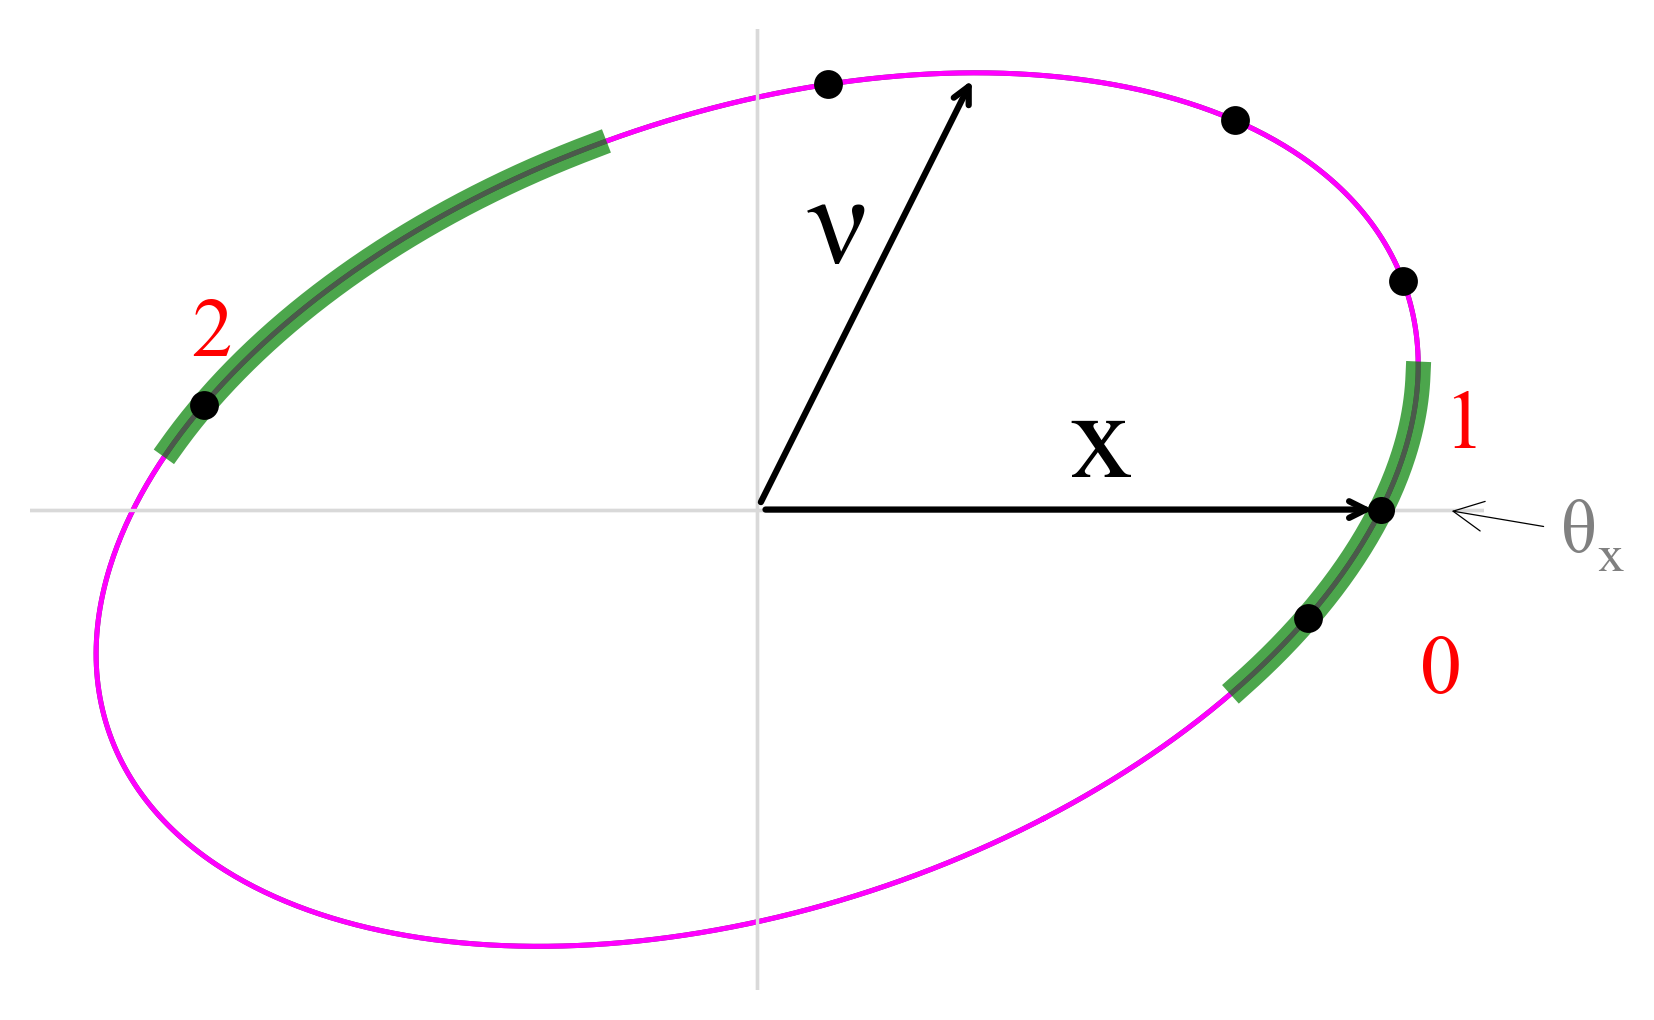
\includegraphics[width=0.4\linewidth]{mess_acceptance_redlabels_valid.png}
    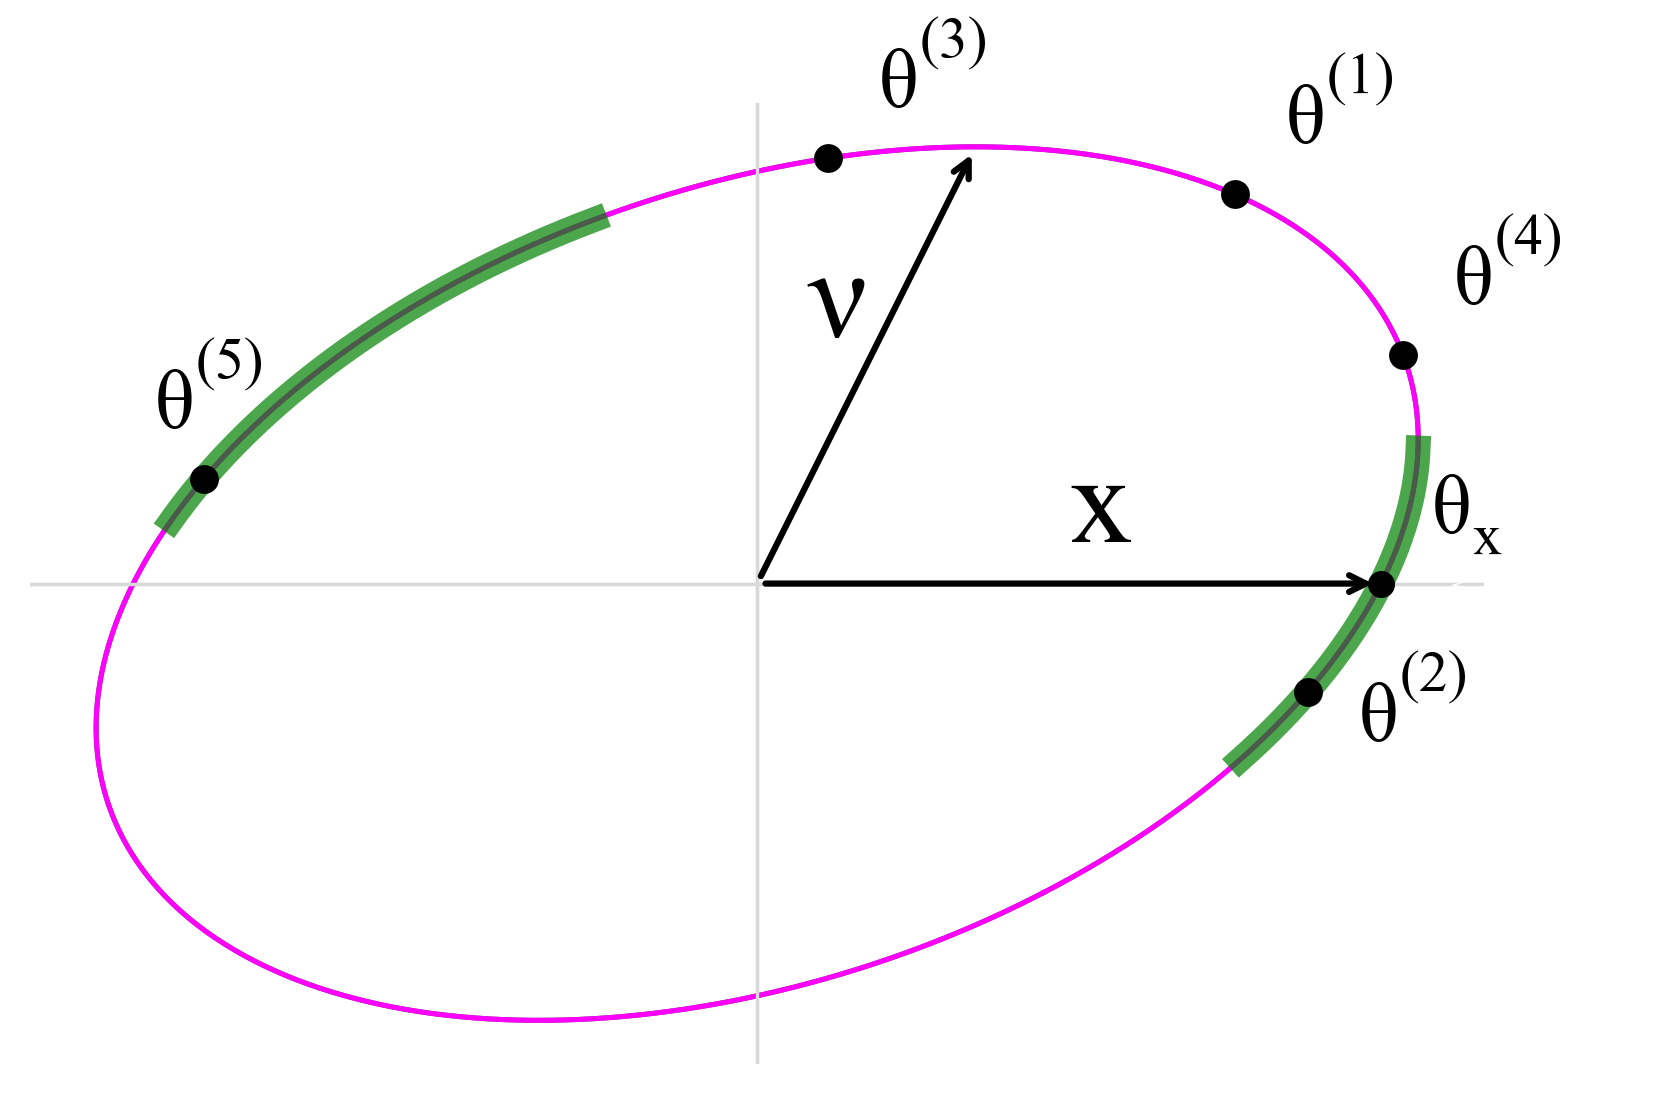
\includegraphics[width=0.4\linewidth]{mess_ellipse_5_proposals.png}
    % \caption{Labels of ordered valid angles.}
\end{figure}
\end{column}
\begin{column}{0.48\textwidth}
% \vspace{-1.3cm}
% \begin{figure}
%     \centering
%     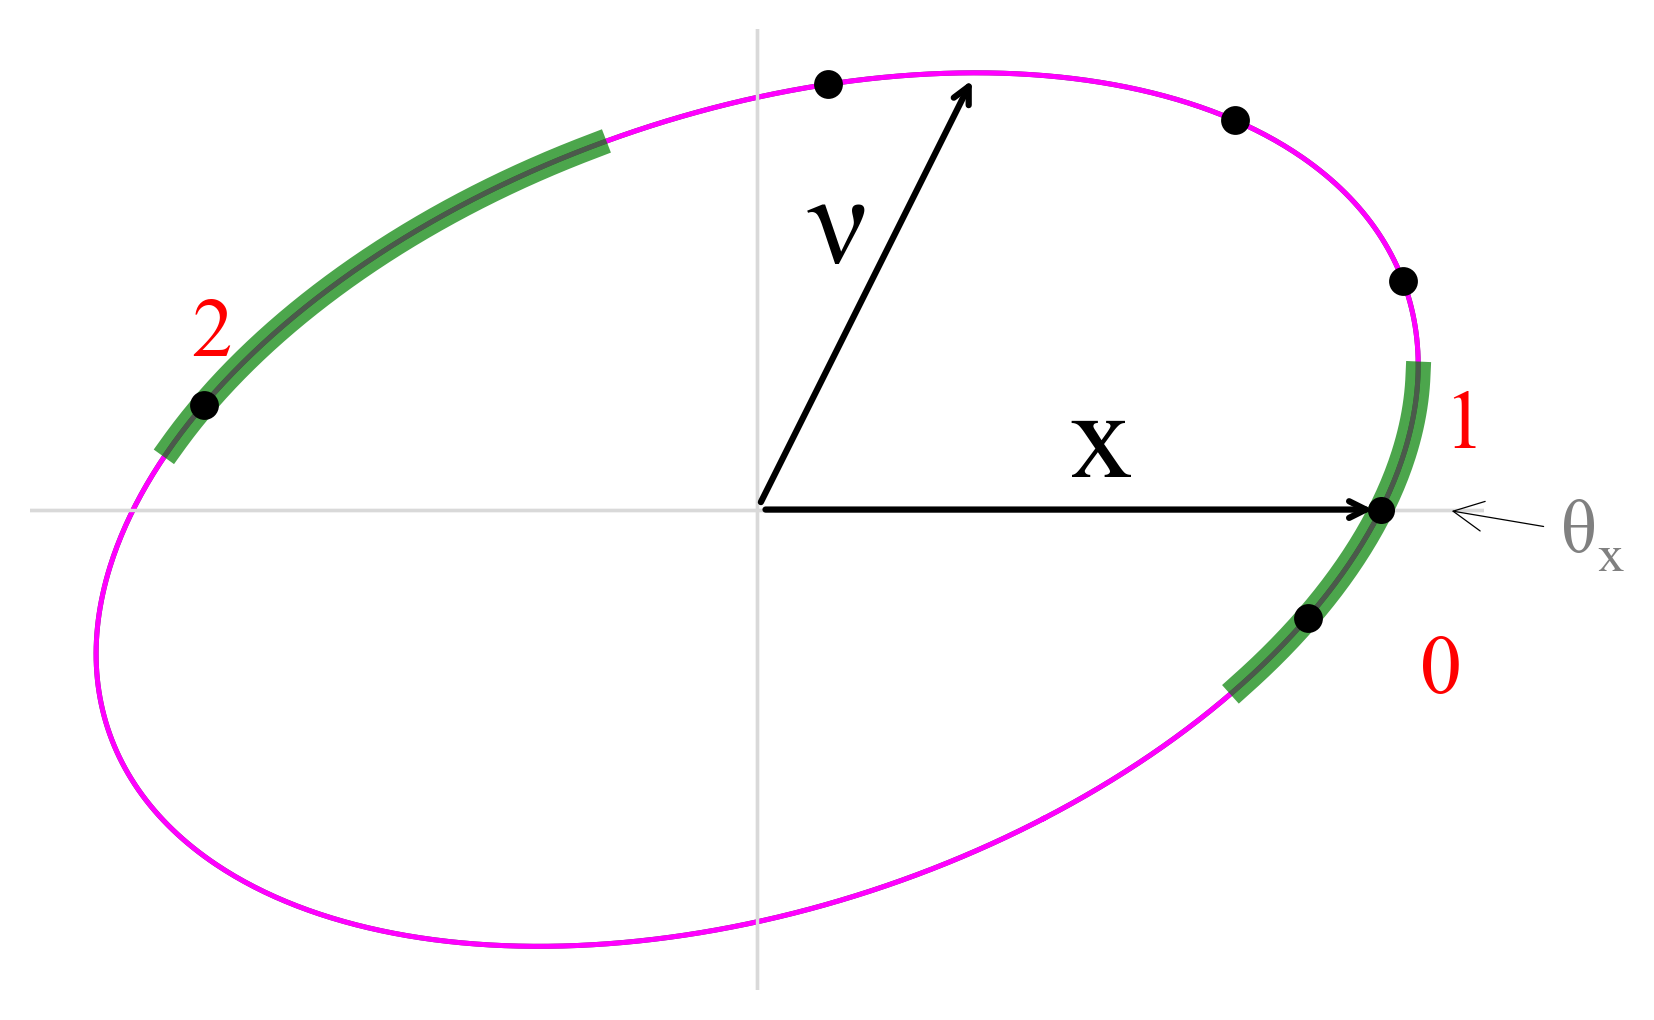
\includegraphics[width=0.4\linewidth]{mess_acceptance_redlabels_valid.png}
%     \caption{Labels of ordered valid angles.}
% \end{figure}
% \vspace{-0.5em}
\begin{itemize}[<+->]
    \item Angular distance matrix:
    \[
    D_{ang} = \begin{bmatrix}
    0 & 0.3 & 3 \\0.3 & 0 & 2.7 \\3 & 2.7& 0
    \end{bmatrix} \quad\mbox{(rad)}
    \]
    \item Example of optimized matrix:
    \[
    \bm{P}^{\star}=
    \begin{bmatrix}
    0 & 1 & 0 \\0 & 0 & 1 \\1 & 0 & 0
    \end{bmatrix}
    \]
\end{itemize}
\end{column}
\end{columns}
\end{frame}

\begin{frame}{Mixing improvement}
\begin{itemize}
    \item Uniform MESS. 
    \item $M$ cores.
    % \item Average number of shrinking steps decays with $M$:
    \begin{figure}
    \centering
    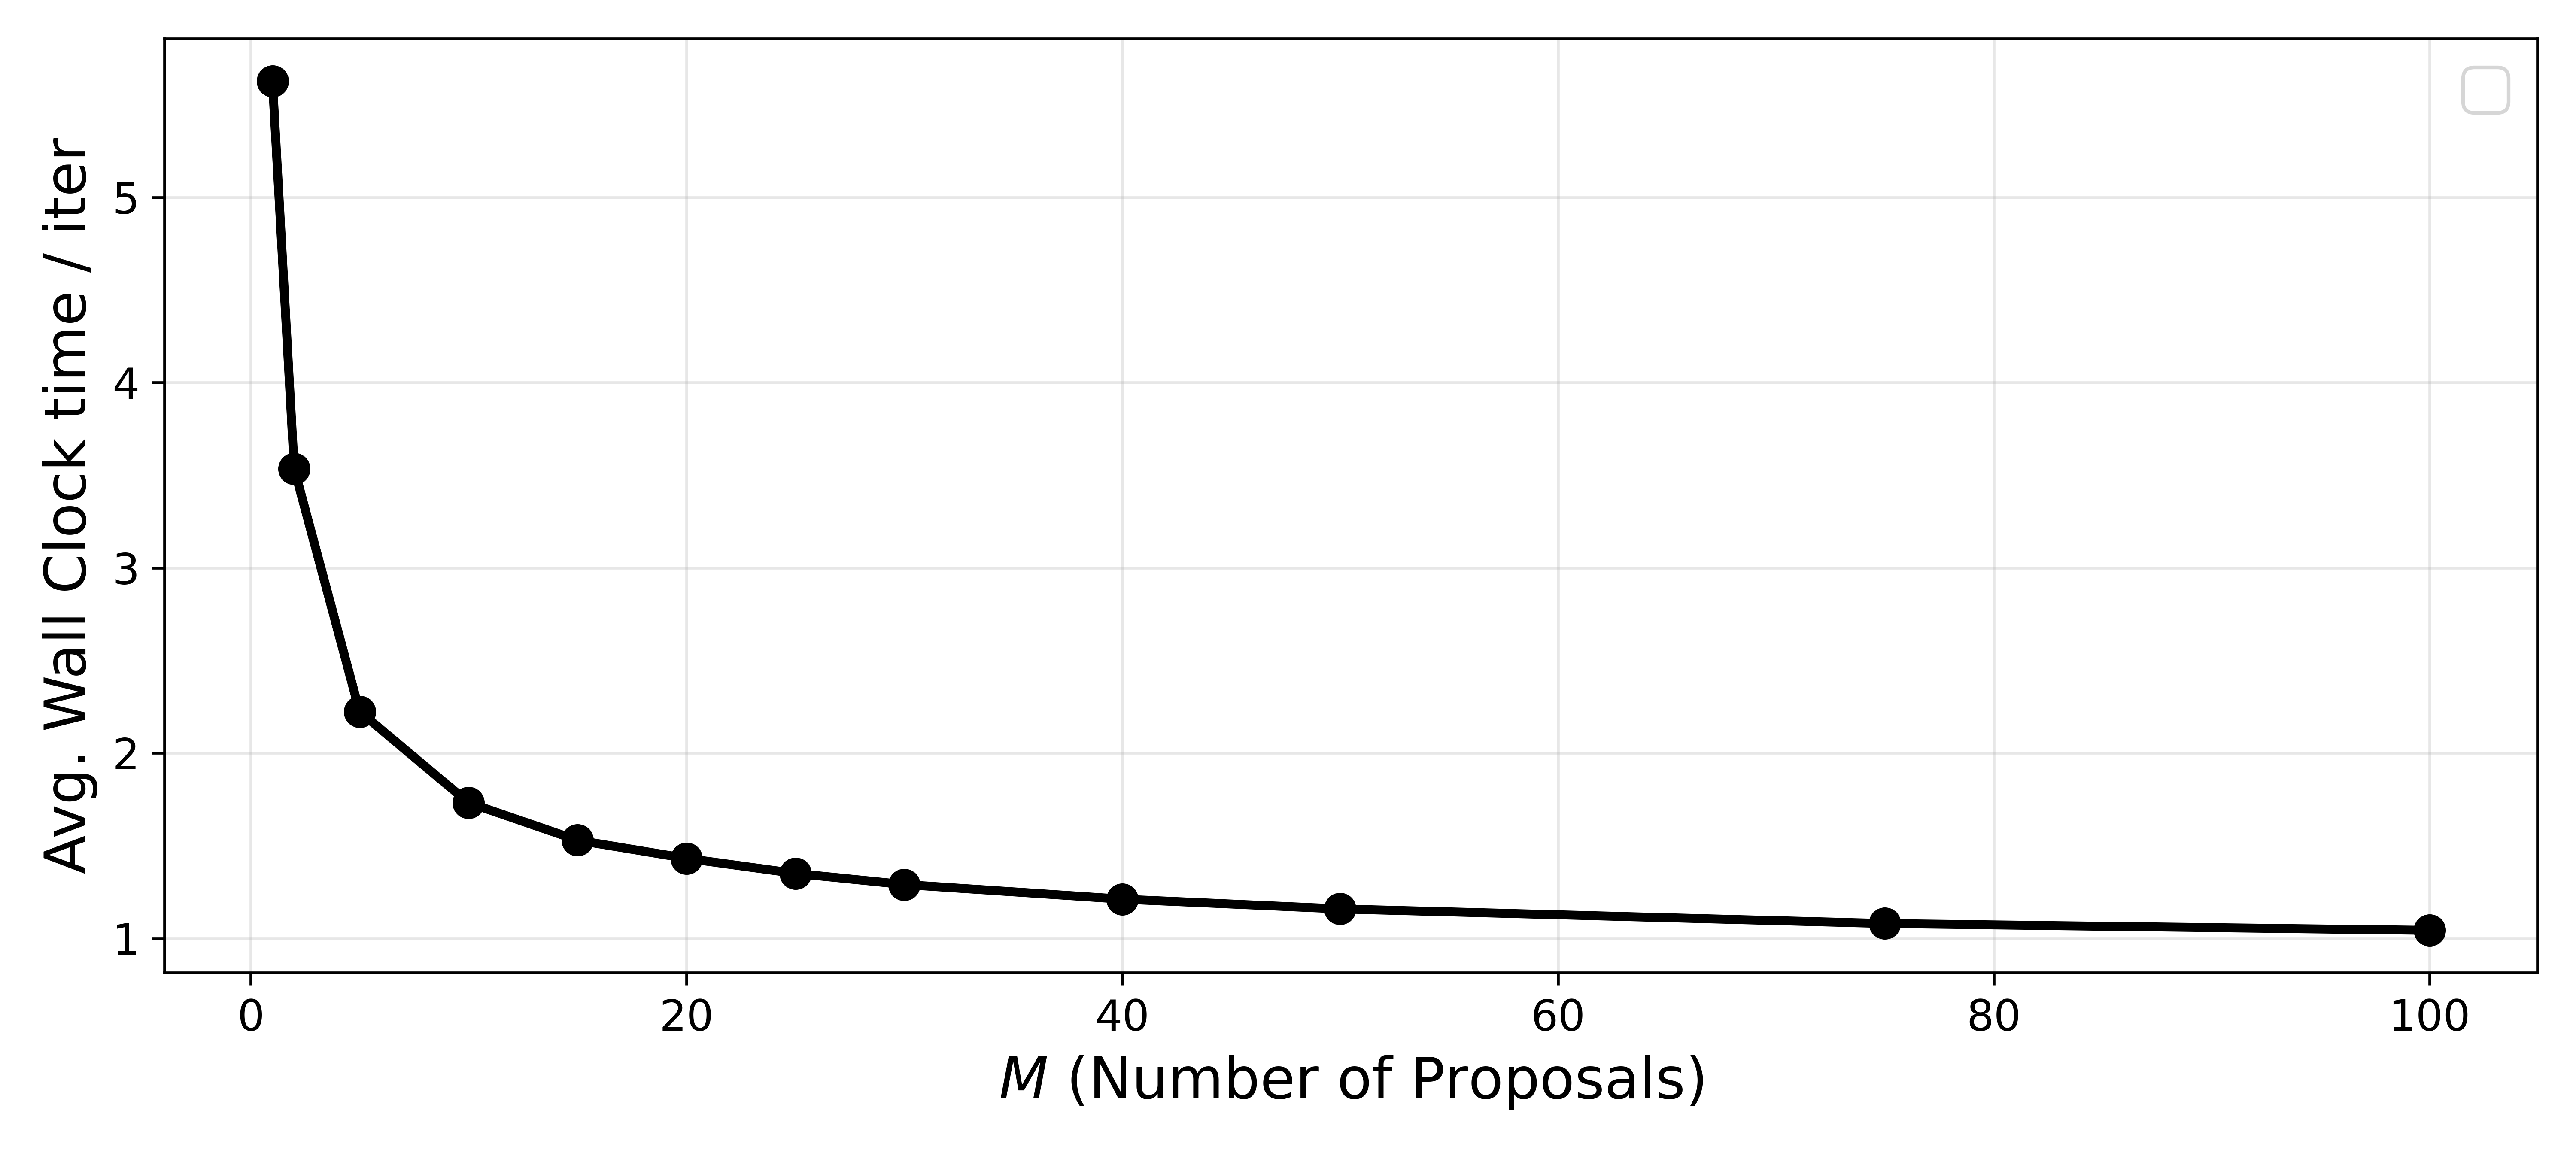
\includegraphics[width=0.7\linewidth]{log_regression_shrinking_considering_parallel_10000iters.png}
    \caption{Average number of subiterations (for a logistic regression model).}
    \end{figure}
    \vspace{0.25em}
    % \item Wall-clock cost per iteration = cost of likelihood x number of shrinking steps.
    % \item With $M$ cores, wall-clock time decreases $\approx$ shrinking steps.
\end{itemize}
\end{frame}

% % --------------------------------
% \begin{frame}{Validity of MESS}
% \begin{itemize}[<+->]
%     \item (I)rreducible because?
%     \vspace{0.25em}
%     \item (R)ecurrent because?
%     \vspace{0.25em}
%     \item (A)periodic because?
%     \vspace{0.25em}
%     \item Proposition: MESS leaves $\pi(\bm{x})$ invariant (ESS is the $M=1$ case).
%     \begin{itemize}[<+->]
%         \item Write joint density of the forward path $(\bm{x},\bm{\nu},y,\alpha,\bm{\varphi}_{1:k},m)$.
%         \item Use a one-to-one, unit-Jacobian transform to the reverse path.
%         \item Bracket update is preserved; double-stochasticity of $\bm{P}$ yields equal marginals.
%     \end{itemize}
%     \vspace{0.25em}
%     \item If we have IRA + invariant distribution, then we have ergodicity.
% \end{itemize}
% \end{frame}

% --------------------------------
% --------------------------------
\section{Results}

\begin{frame}{Solute transport model\footnote{From \citet{GlattHoltz2024}.}}
    % spectral discretization of an advection–diffusion type equation.
    \begin{columns}
    \begin{column}{0.6\textwidth}
        \begin{itemize}[<+->]
        \item Mimics transportation of a solute by a fluid under damping and external forcing. 
        \begin{equation*} 
            \frac{d\bm{s}}{dt} + (\bm{A} + \kappa \bm{I}_d) \bm{s} = \bm{g}.
        \end{equation*}
        \begin{itemize}[<+->]
            \item $\bm{s} \in \mathbb{R}^d$: Concentration.
            \item $\bm{g}=(1,0,\ldots,0) \in \mathbb{R}^d$: Forcing.
            \item $\kappa \in \mathbb{R}$: Damping.
            \item $\bm{A} \in \mathbb{R}^{d\times d}$: Spectral transport matrix. %advection by the air flow.
            % \begin{itemize}[<+->]
                % \item Zero-diagonal.
                % % \item How concentration at one spatial scale influences another scale.
                % \item Antisymmetric.
            % \end{itemize}
        \end{itemize}
        \item Steady state:
        \[
        \bm{s}(\bm{A}) = (\bm{A}+\kappa \bm{I}_d)^{-1}\bm{g}.
        \]        
    \end{itemize}
    \end{column}
    \begin{column}{0.4\textwidth}
    \vspace{-0.1cm}
    \begin{figure}
    \centering
    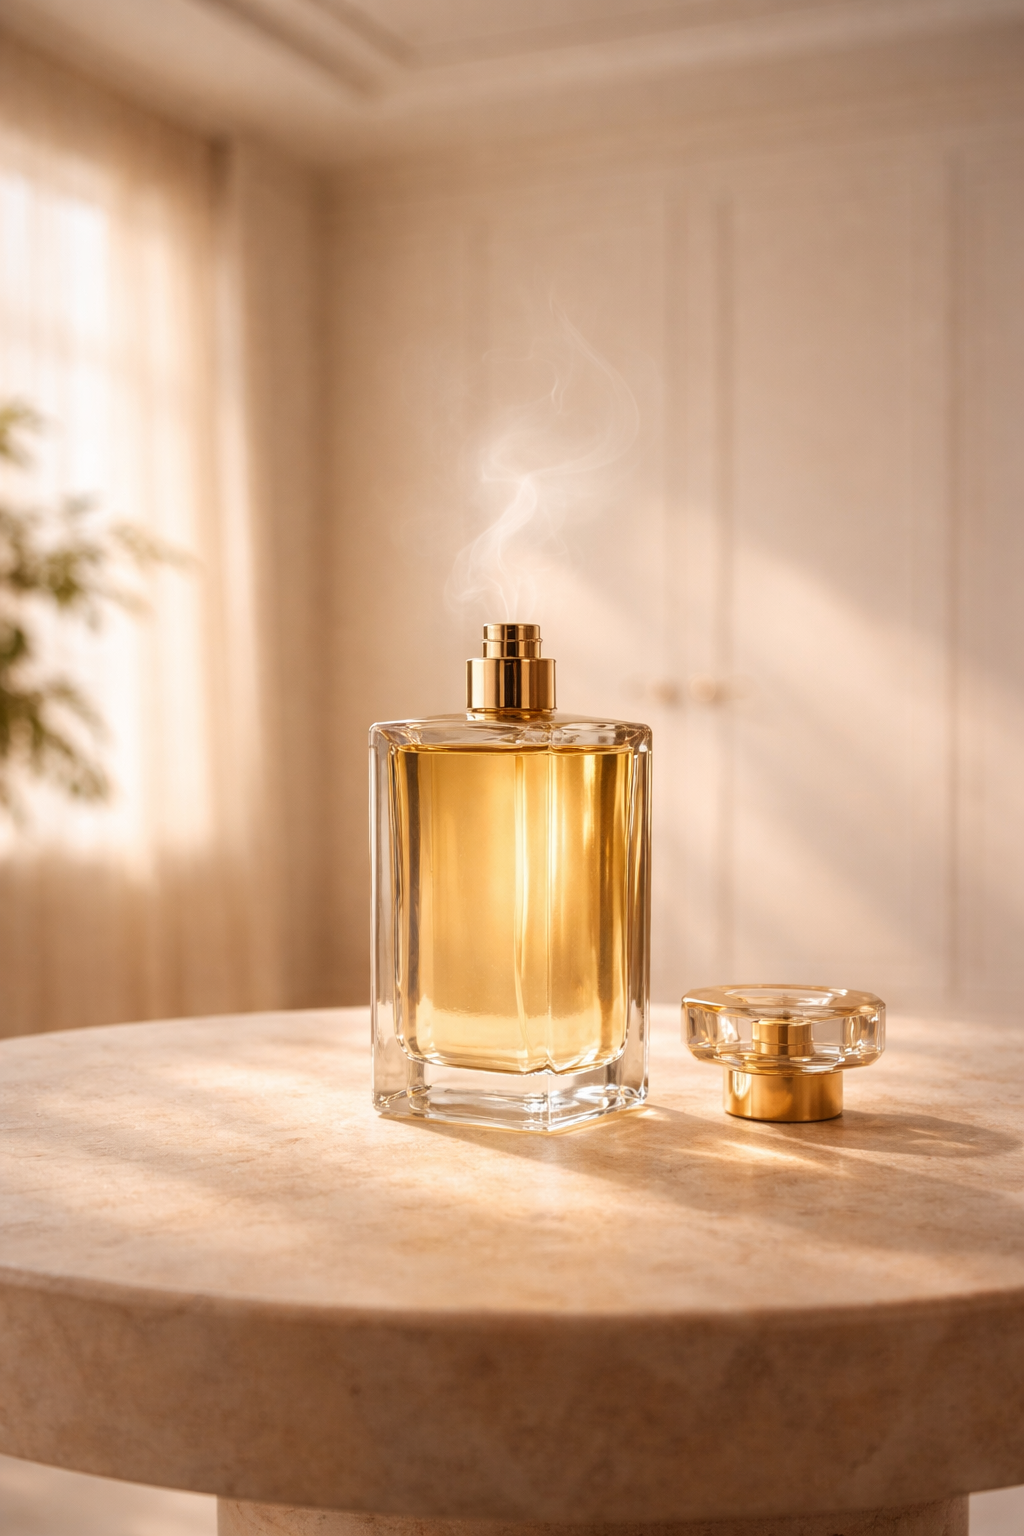
\includegraphics[width=0.6\linewidth]{perfume.png}
    % \caption{Example.}
    \end{figure}
    \end{column}
    \end{columns}
\end{frame}

\begin{frame}{Bayesian inverse problem}
    \begin{columns}
    \begin{column}{0.6\textwidth}
    % Goal: Infer $A$ from noisy observations of $\Theta(A) = (A+\kappa I)^{-1}g$.
    \begin{itemize}[<+->]
        \item Gaussian prior on the non-zero elements of $\bm{A}$:
        \[
        \bm{A} \sim N(0, \bm{C}), \quad \bm{C} = \mbox{diag}(\{\mbox{Var}(a_{ij})\}). %\quad\quad\Rightarrow \pi(\bm{A});
        \]
        \begin{itemize}[<+->]
        \item Zero-diagonal.
                % \item How concentration at one spatial scale influences another scale.
        \item Antisymmetric.
        \item $m=d(d-1)/2$ elements in upper triangle;
        % \item Contains Fourier coefficients of the concentration field.
        \item $\bm{C}$ penalizes long range interactions and high frequencies.
        \end{itemize}
        \item Gaussian likelihood:
        \begin{equation*}
            \mathbf{\mathsf{y}} = \bm{s}(\bm{A}) + \bm{\eta}, \quad \bm{\eta} \sim N(0, \sigma^2 \bm{I}_d). %\quad\quad\quad\Rightarrow \mathcal{L}(\bm{\mathsf{y}}|\bm{A}),
        \end{equation*}
        % \begin{itemize}
        % \item Optional projection $\mathcal{P}$:
        %     \begin{equation*}
        %         \mathbf{\mathsf{y}}_k = \mathcal{P}(\mathbf{\mathsf{y}}) \in \mathbb{R}^k, k\leq d 
        %     \end{equation*}
        % \end{itemize}
        % \item Likelihood:
        % \[
        % y = \bm{s}(A) + \epsilon, \quad \epsilon \sim N(0, \sigma^2 I).
        % \]
        \item Posterior:
        \[
        \pi(\bm{A}|\mathbf{\mathsf{y}}) \propto \mathcal{L}(\mathbf{\mathsf{y}}|\bm{A}) \pi_0(\bm{A}).
        \]
    \end{itemize}
    % \end{itemize}
    \end{column}
    \begin{column}{0.4\textwidth}
    \vspace{-2cm}
    \begin{figure}
        \centering
        \onslide<1->{
            \begin{subfigure}[b]{0.6\linewidth}
                \centering
                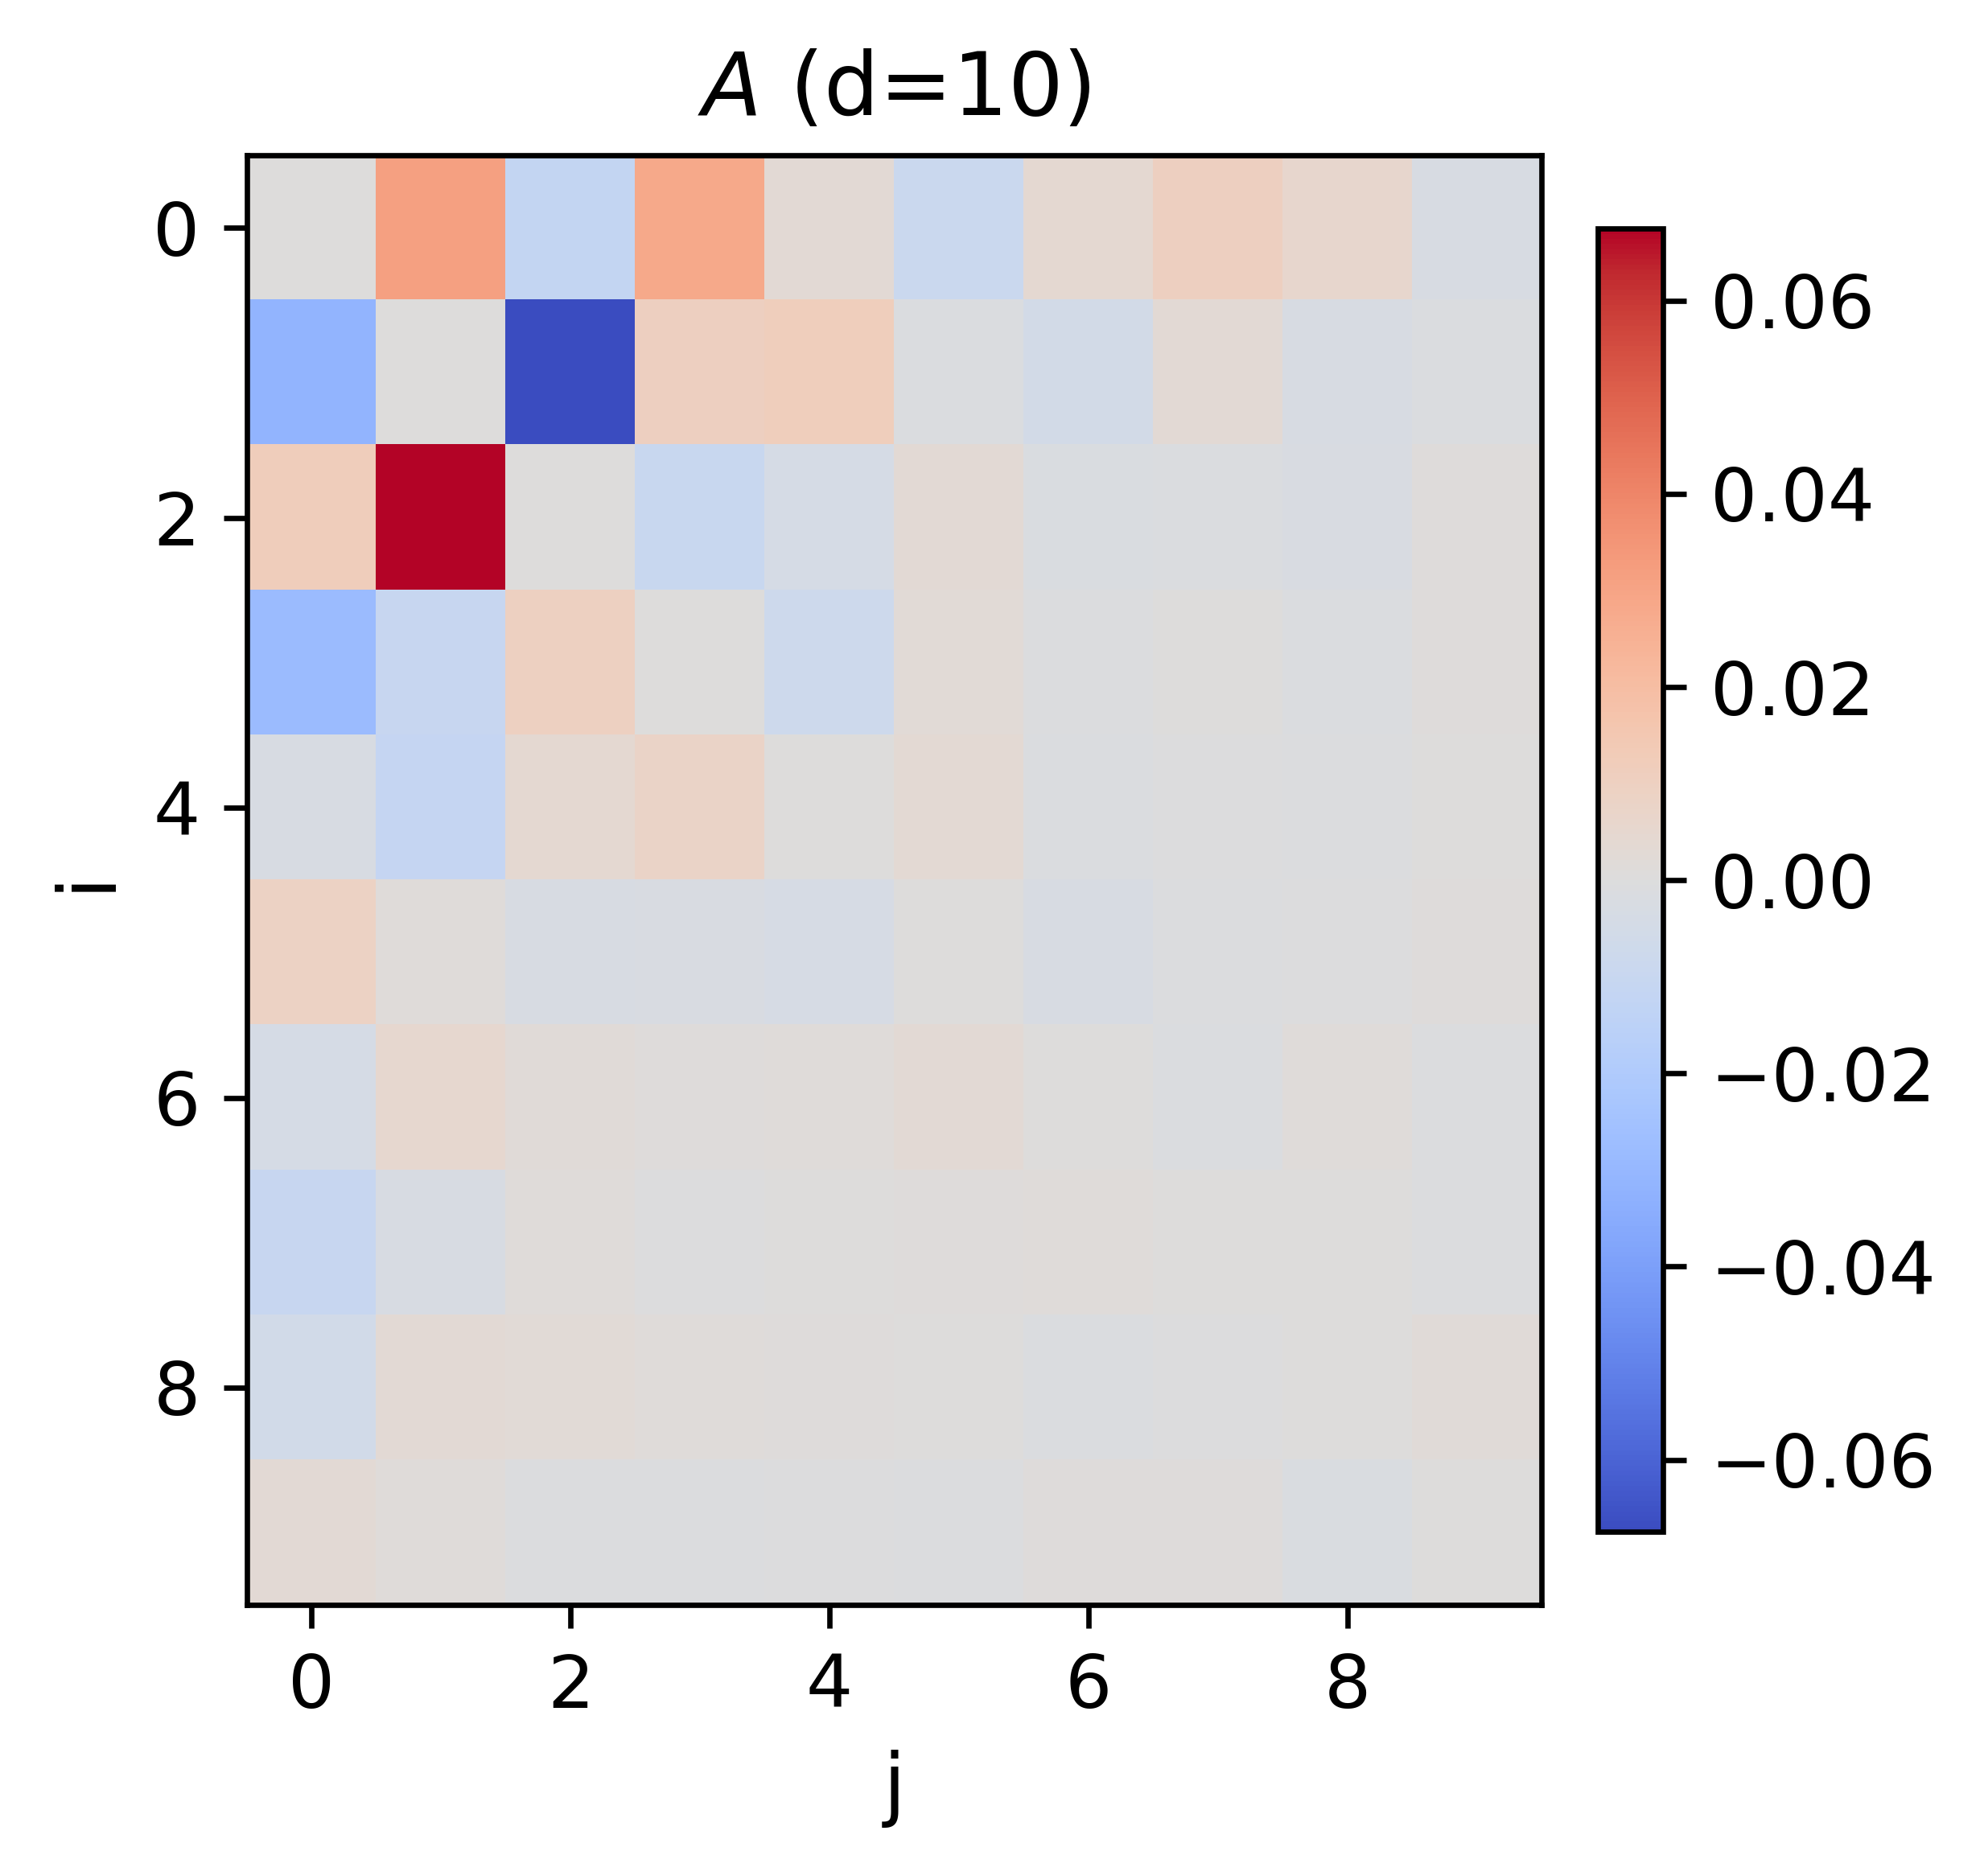
\includegraphics[width=\linewidth, trim={0 0 0 0.8cm}, clip]{visual_check_A_d10.png}
                \caption{$\bm{A}_{10}$.}
            \end{subfigure}
        }
        \onslide<4->{
            \begin{subfigure}[b]{0.6\linewidth}
                \centering
                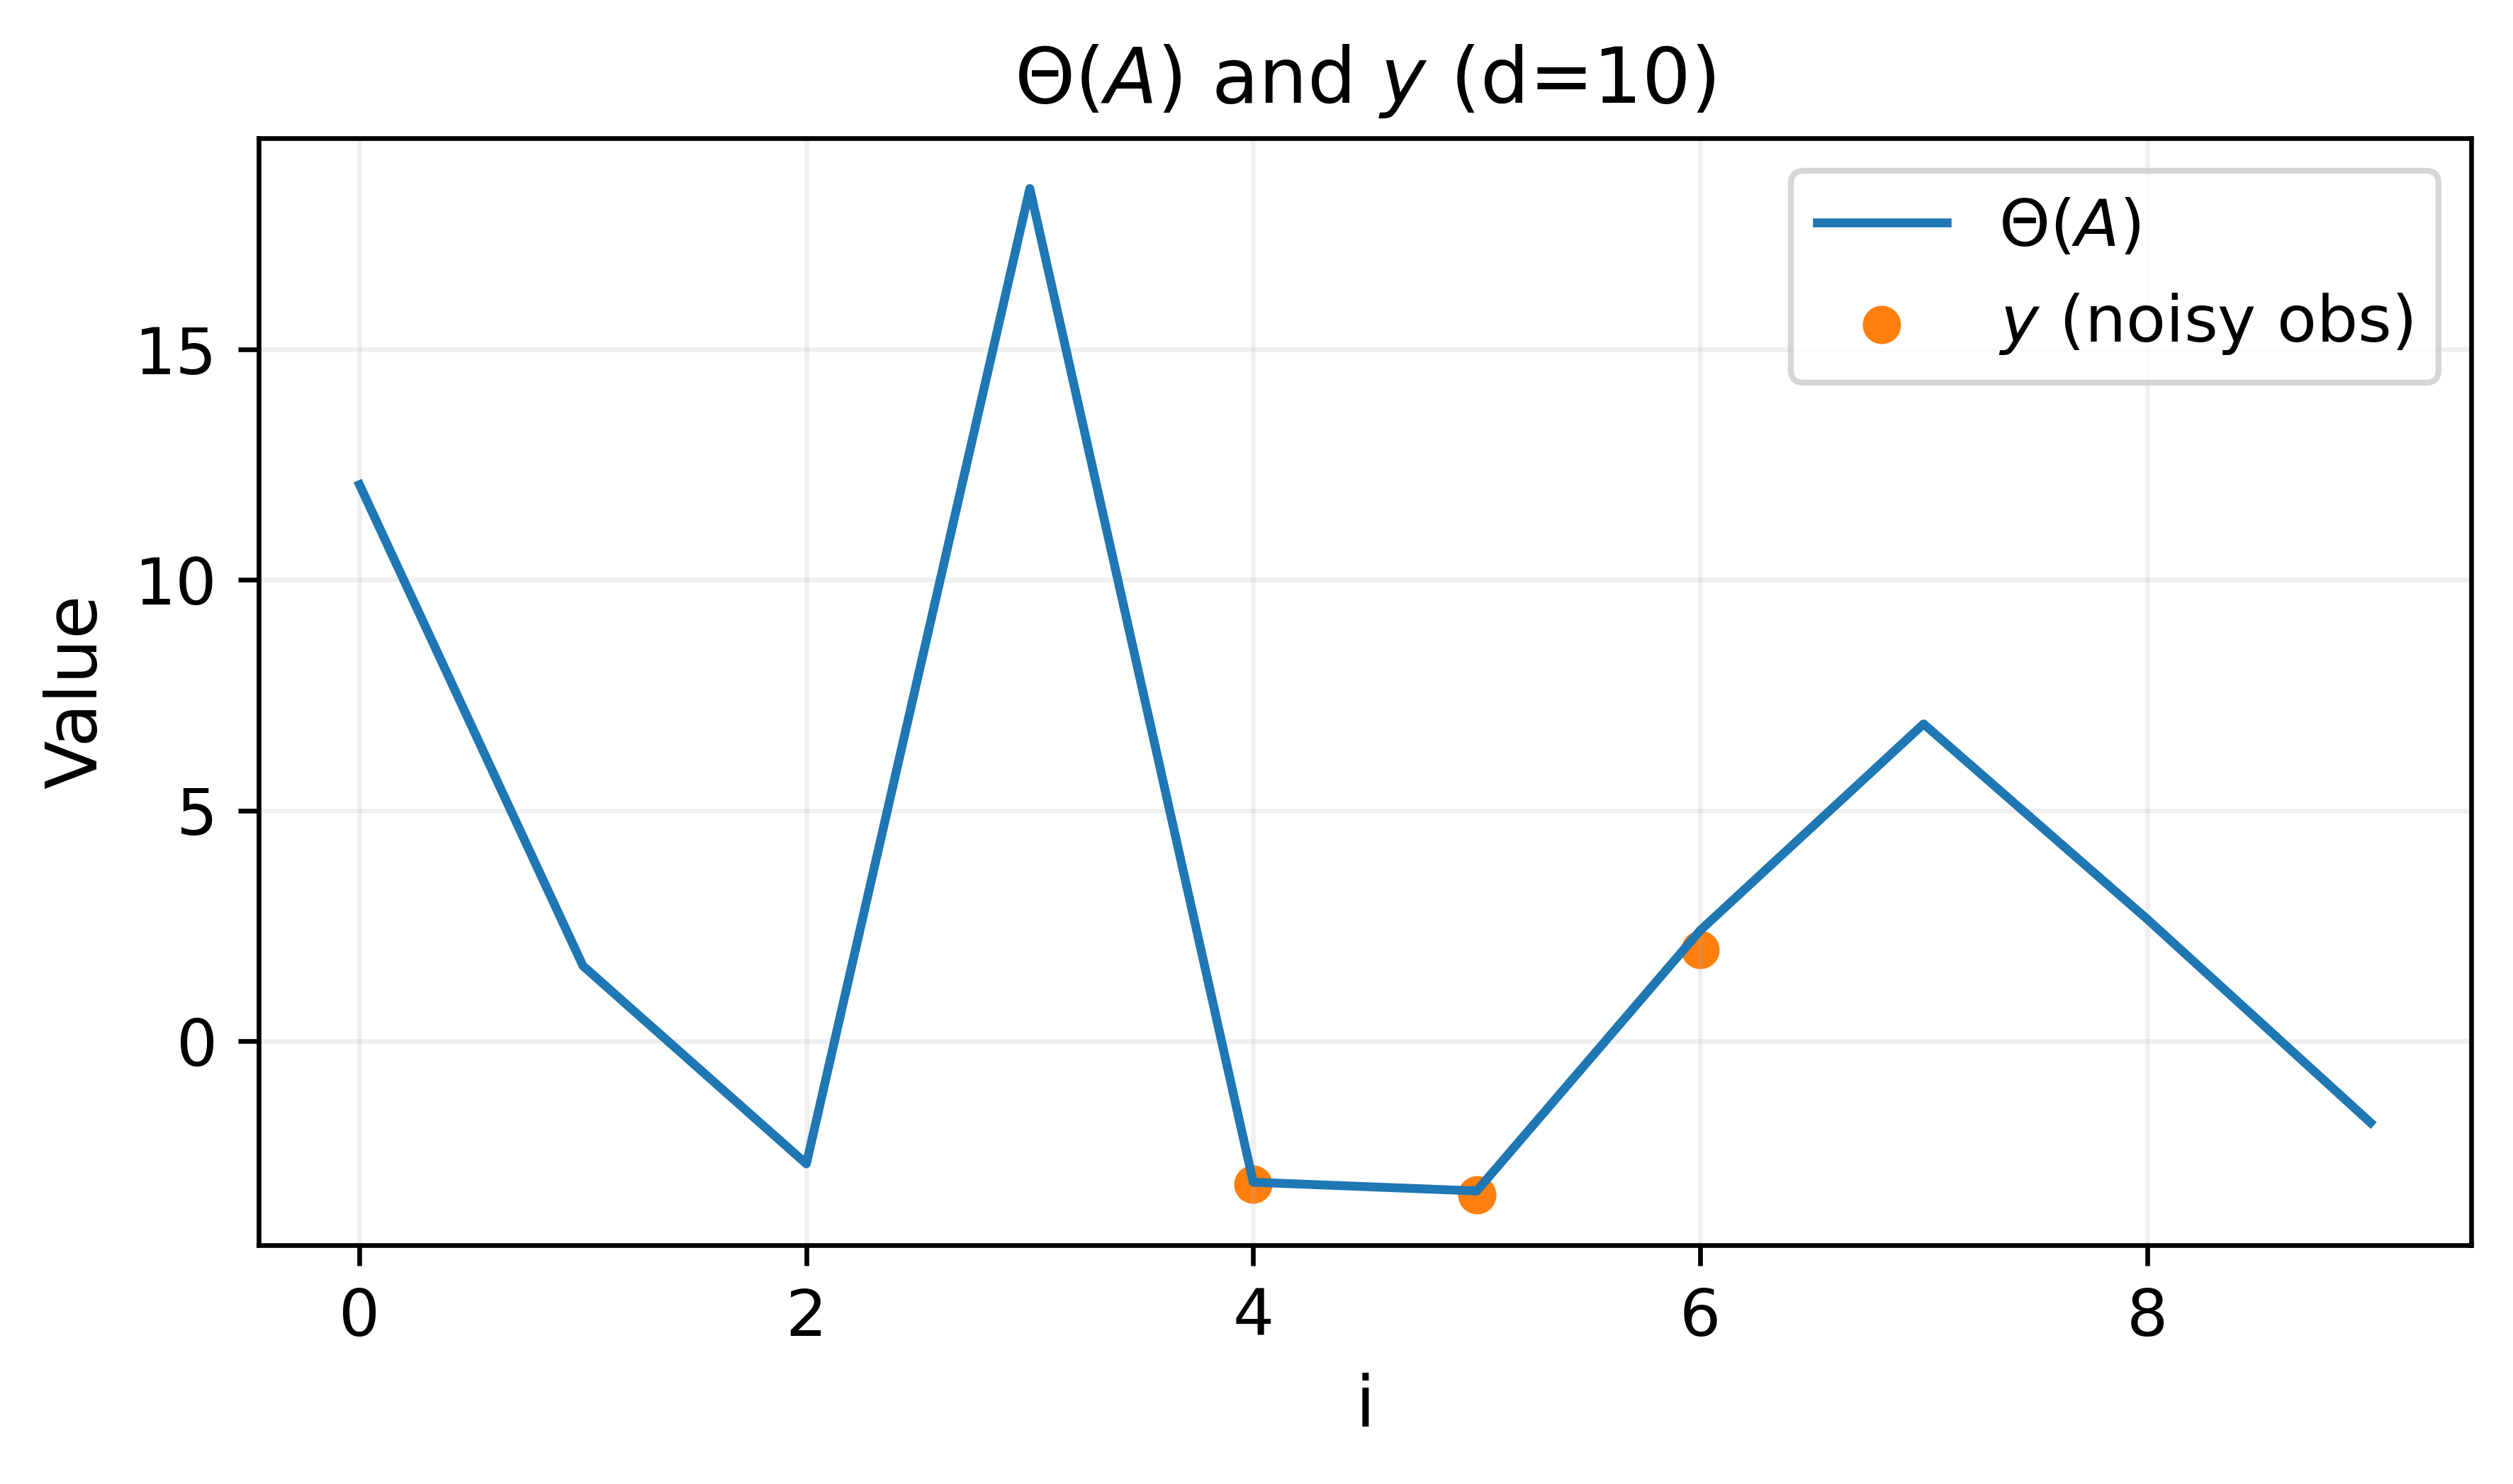
\includegraphics[width=\linewidth, trim={0 0 0 0.8cm}, clip]{visual_check_theta_y_d10.png}
                \caption{$\bm{s}(\bm{A}_{10})$ and $\bm{\mathsf{y}}_3$.}
            \end{subfigure}
        }
    \end{figure}
    \end{column}
    \end{columns}
\end{frame}

% \begin{frame}{Simulations from the model}
% \begin{figure}
%     \centering
%     \begin{subfigure}[b]{0.4\linewidth}
%         \centering
%         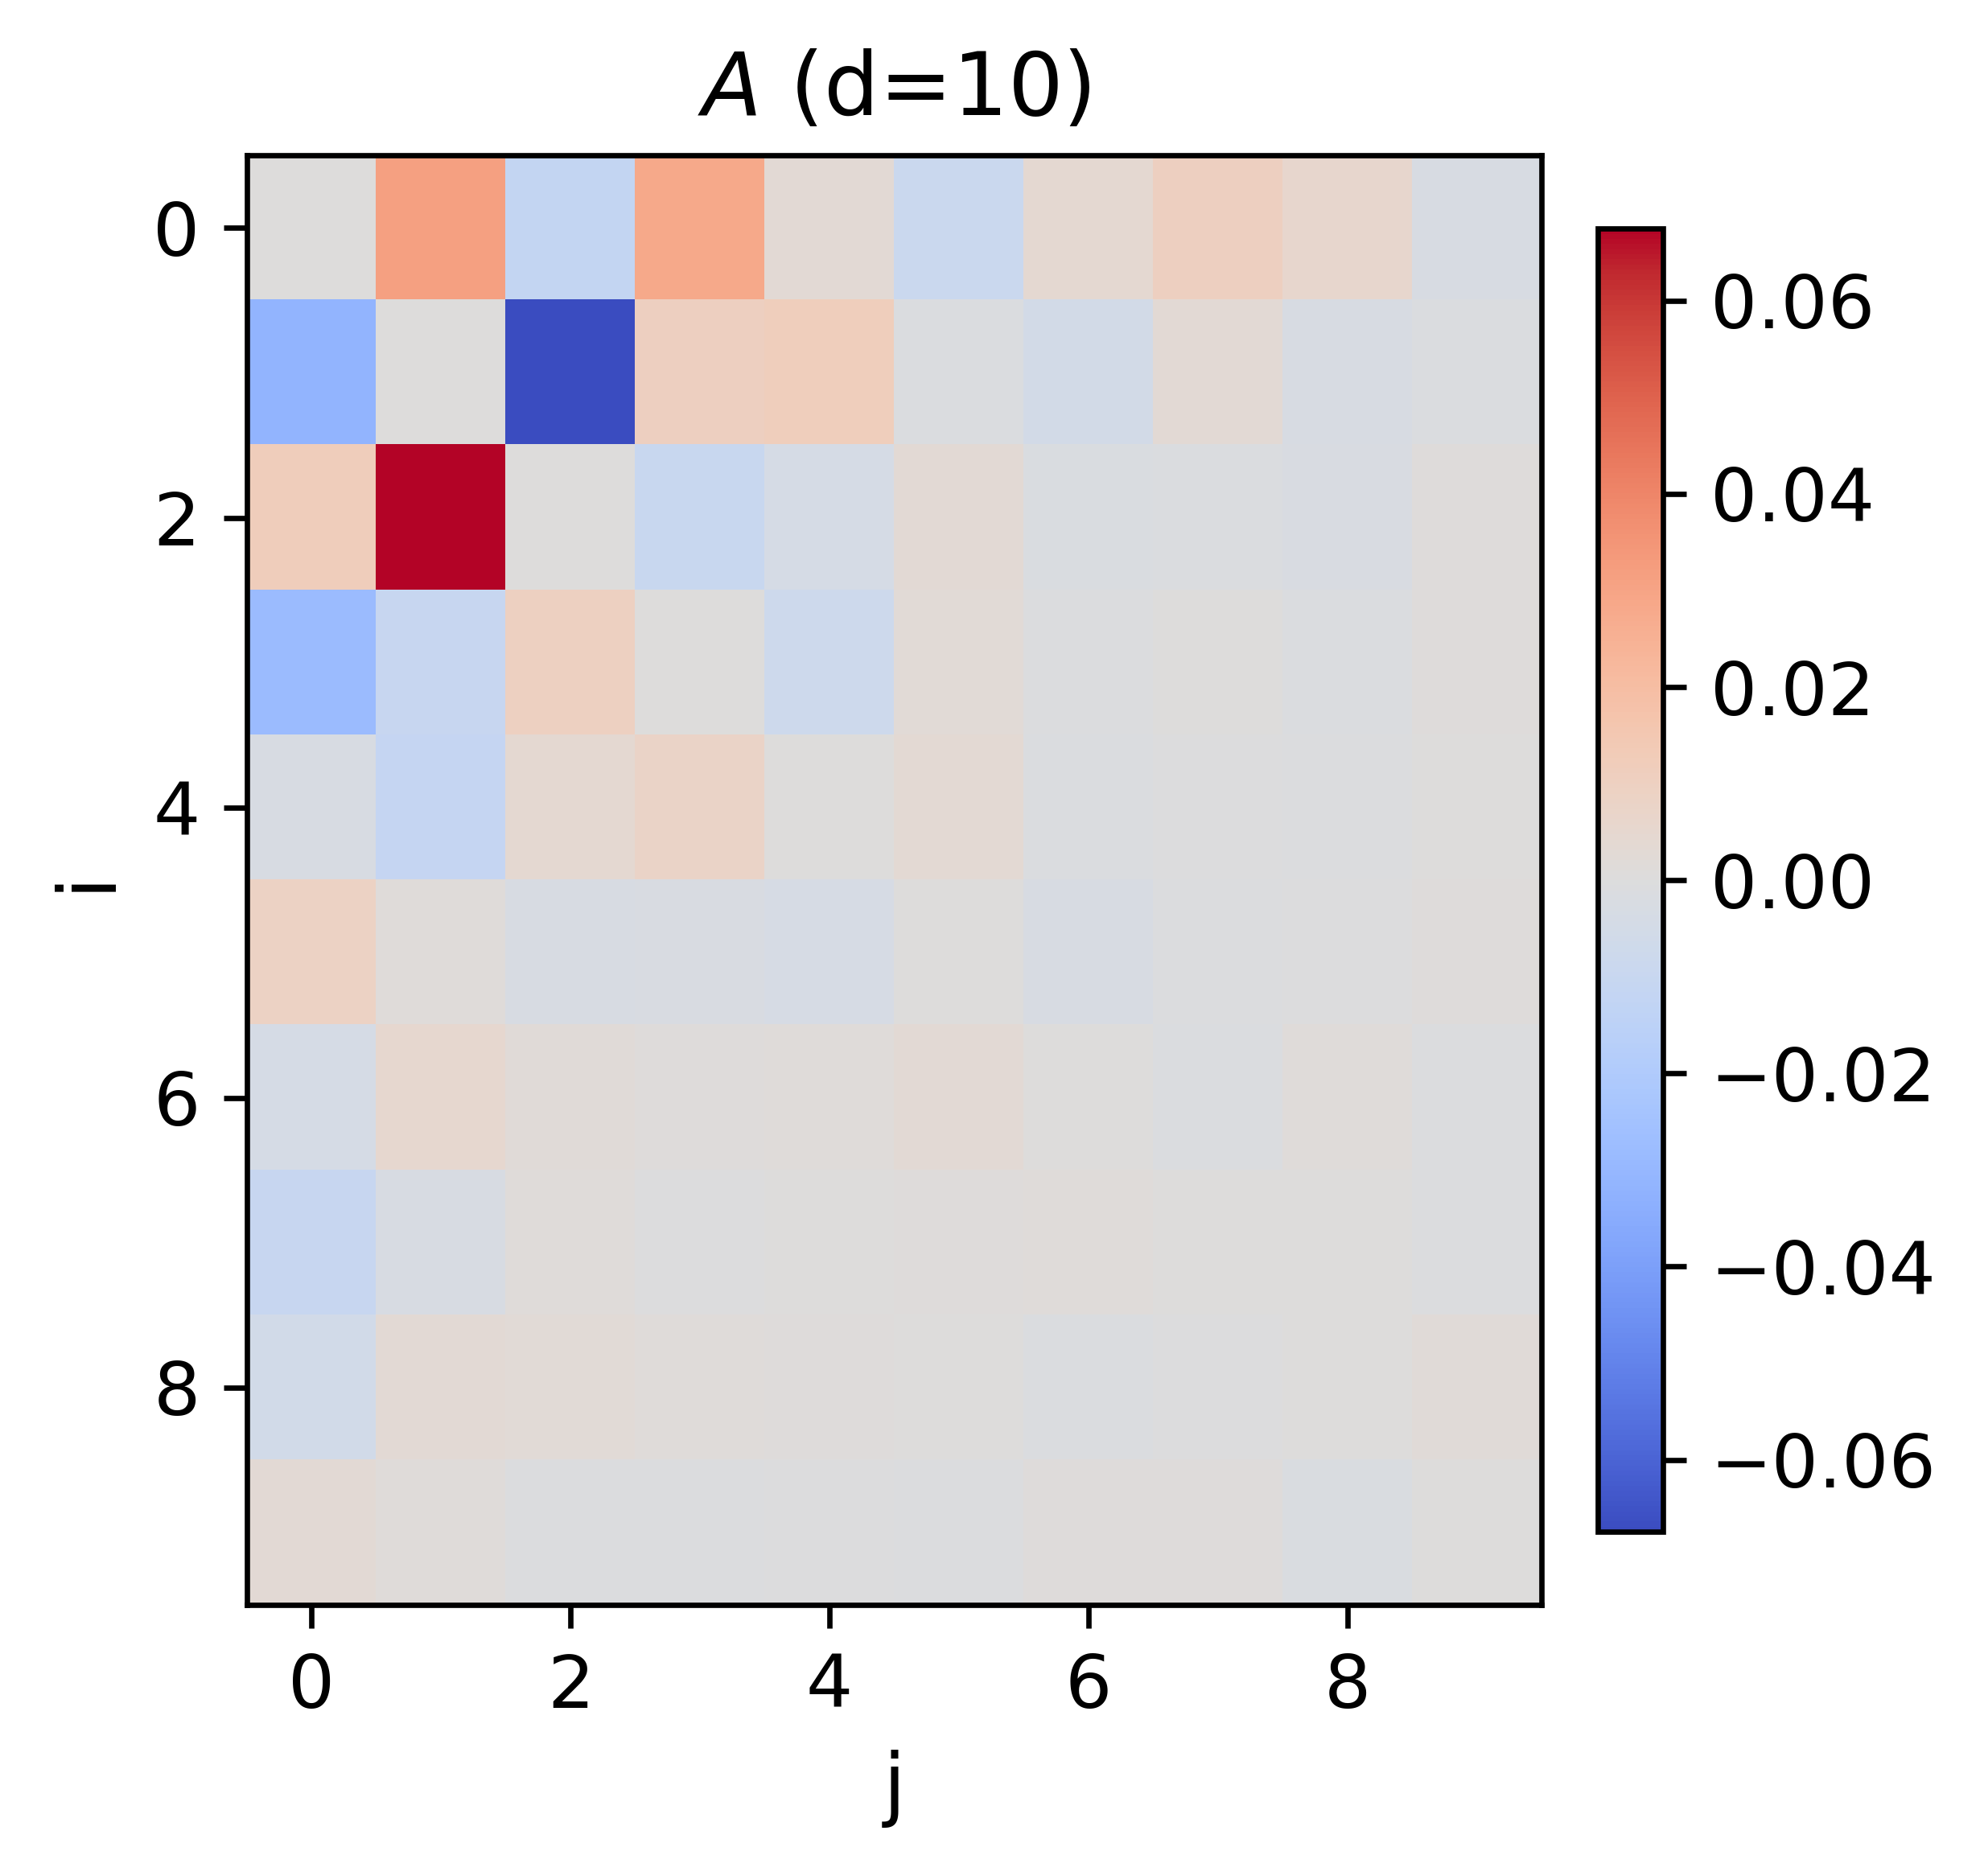
\includegraphics[width=\linewidth, trim={0 0 0 0.8cm}, clip]{visual_check_A_d10.png}
%         \caption{$A_{10}$.}
%     \end{subfigure}
%     % \hfill
%     % \vspace{1cm}
%     \begin{subfigure}[b]{0.4\linewidth}
%         \centering
%         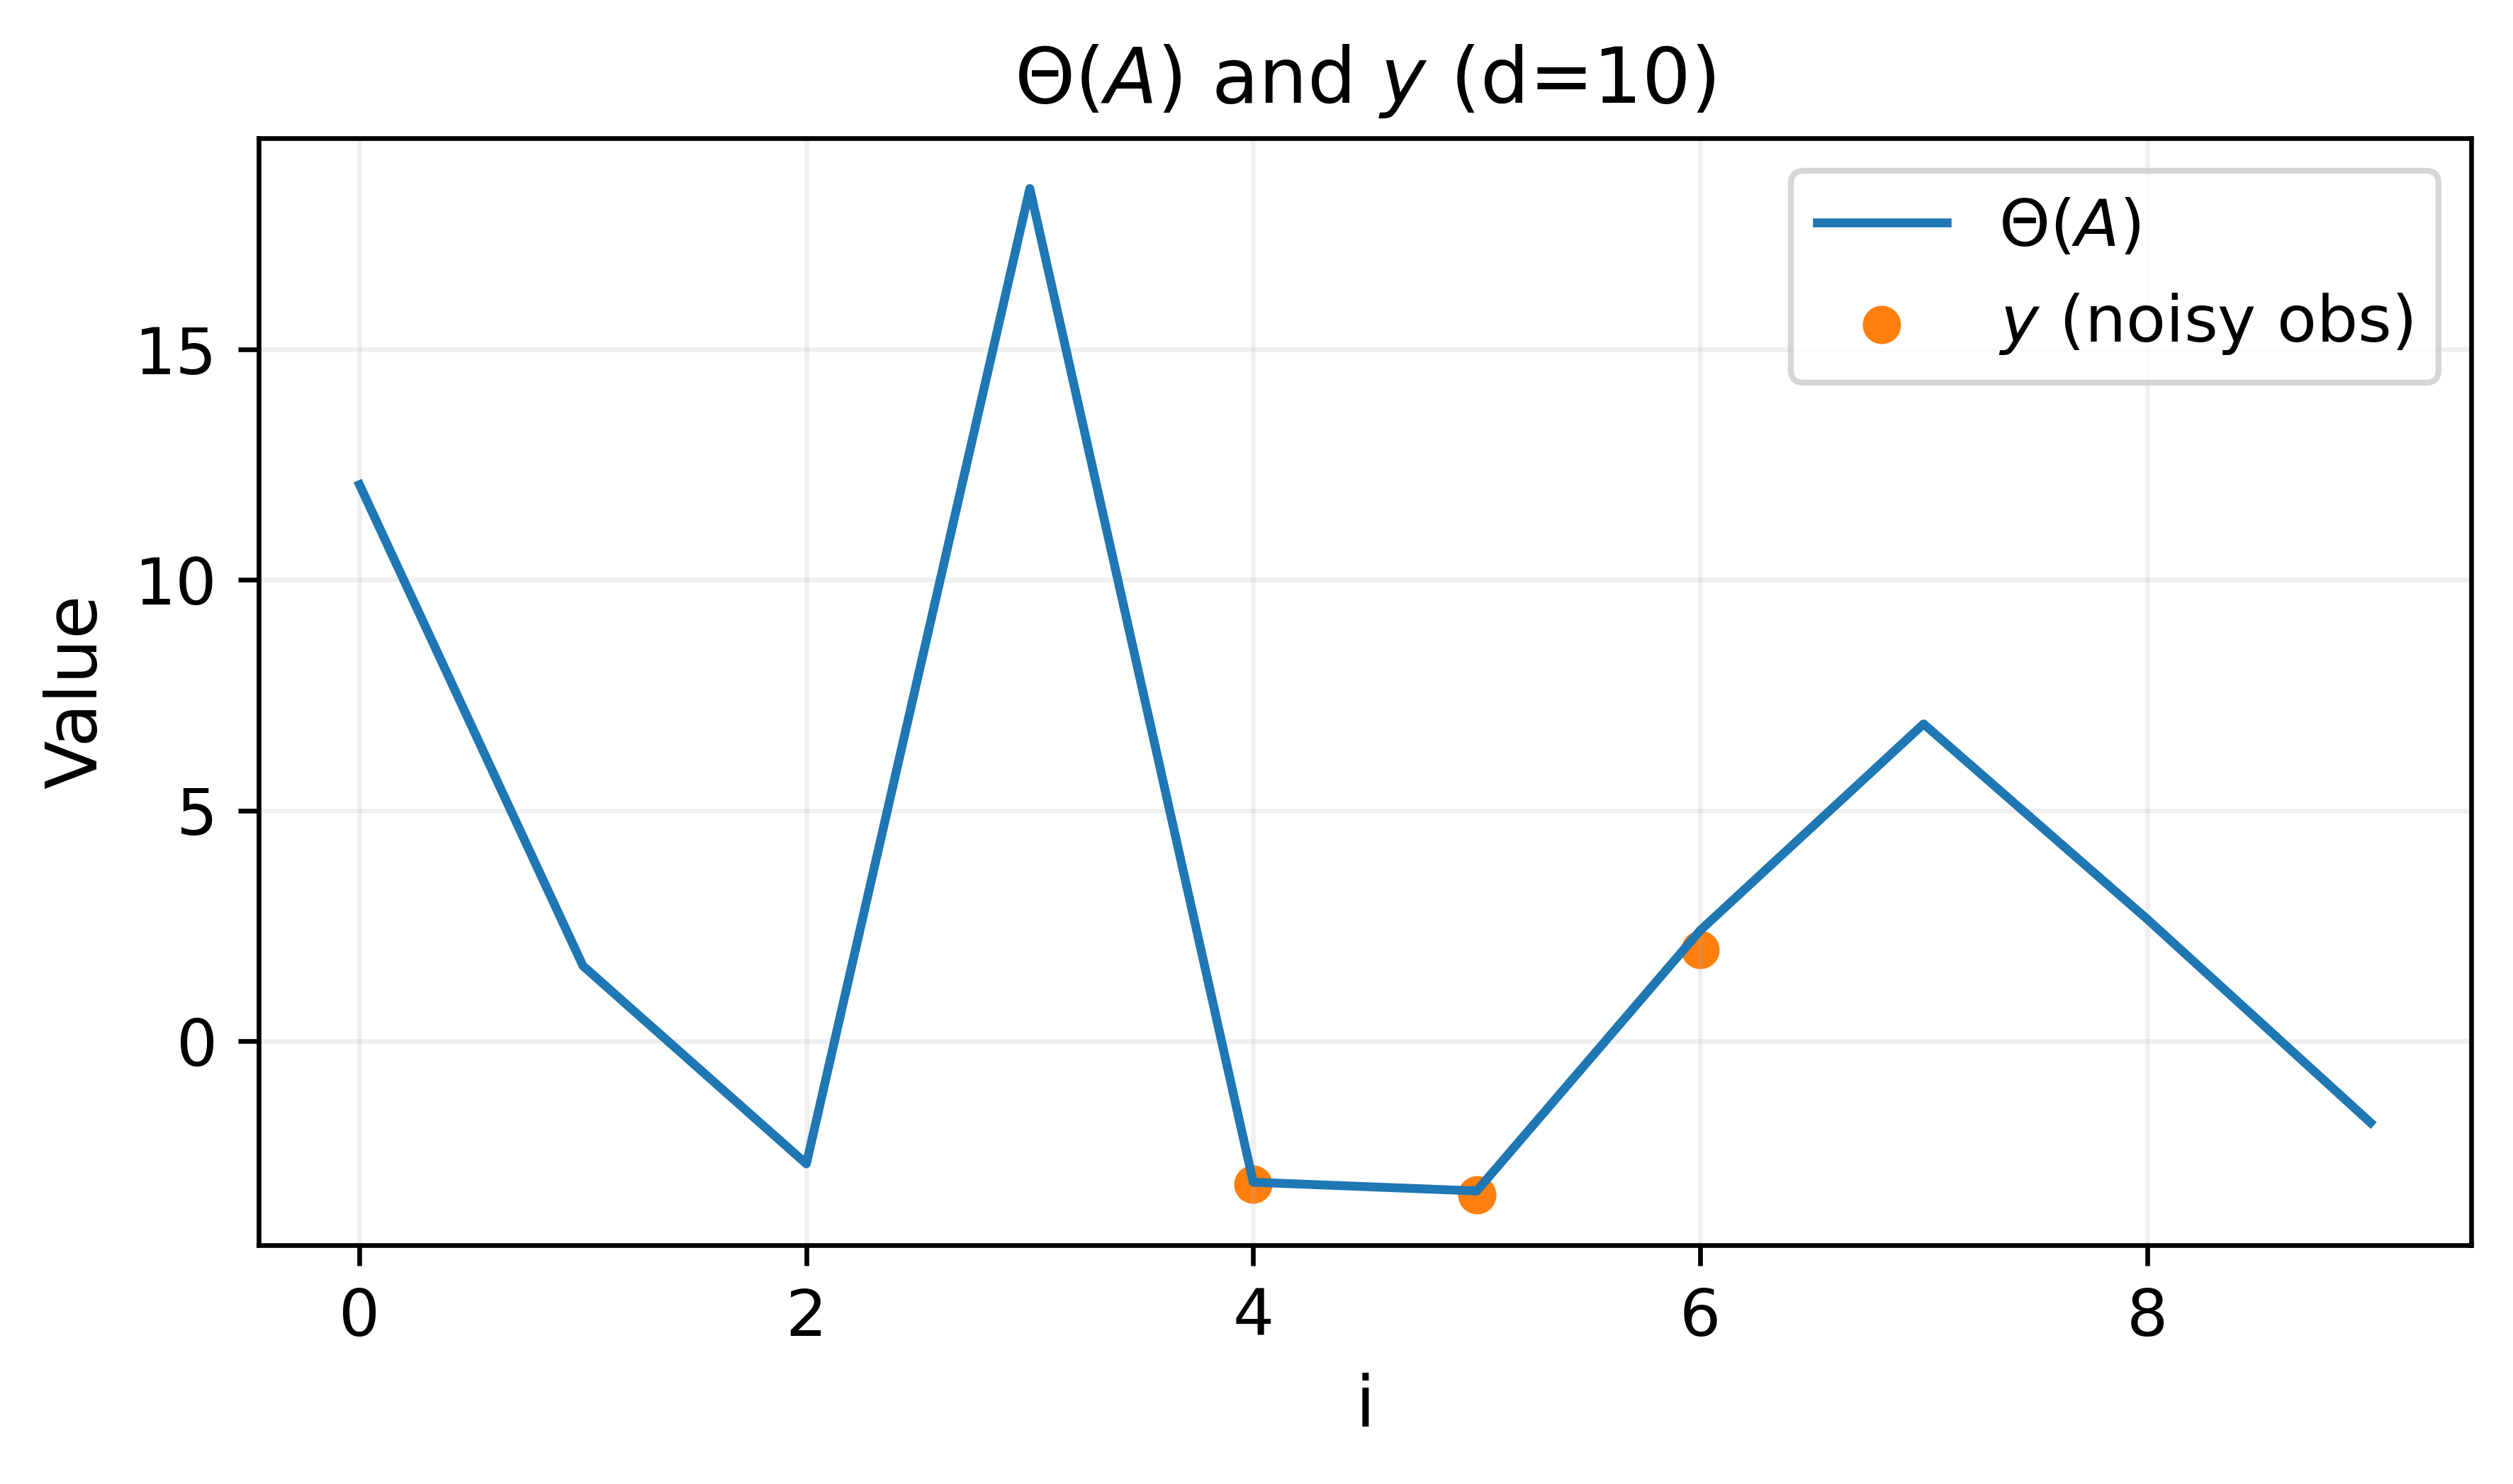
\includegraphics[width=\linewidth, trim={0 0 0 0.8cm}, clip]{visual_check_theta_y_d10.png}
%         \caption{$\Theta(A_{10})$ and $\mathsf{y}_3$.}
%     \end{subfigure}
% \end{figure}
% \end{frame}
% \begin{frame}{Simulations from the model}
% \begin{columns}
% \begin{column}{0.5\textwidth}
% \begin{itemize}[<+->]
%     % \item $A$ is $d \times d$, antisymmetric, zero diagonal.
%     % \item Specified by the $m=d(d-1)/2$ non-zero elements in the upper triangle.
%     % \item Prior on these elements:
%     % \[
%     %     a_{ij} \sim \mathcal{N}(0,\mbox{Var}(a_{ij})),
%     % \]
%     % \[
%     %     \mbox{Var}(a_{ij})=\tau^2 (ij)^{-\alpha}|i-j|^{-\gamma}.
%     % \]
%     % \item Therefore
%     % \[
%     % A \sim N(0, C), \quad C = \mbox{diag}(\{\mbox{Var}(a_{ij})\})
%     % \]
%     % \vspace{0.25em}
%     % \item Covariance $C$ penalizes long range interactions and high frequencies.
%     % \item Choose $\tau^2=1$, $\alpha=3$, $\gamma=w$.
% \end{itemize}
% \end{column}
% \begin{column}{0.5\textwidth}
% \vspace{-1cm}
% \begin{figure}
%     \centering
%     \begin{subfigure}[b]{0.6\linewidth}
%         \centering
%         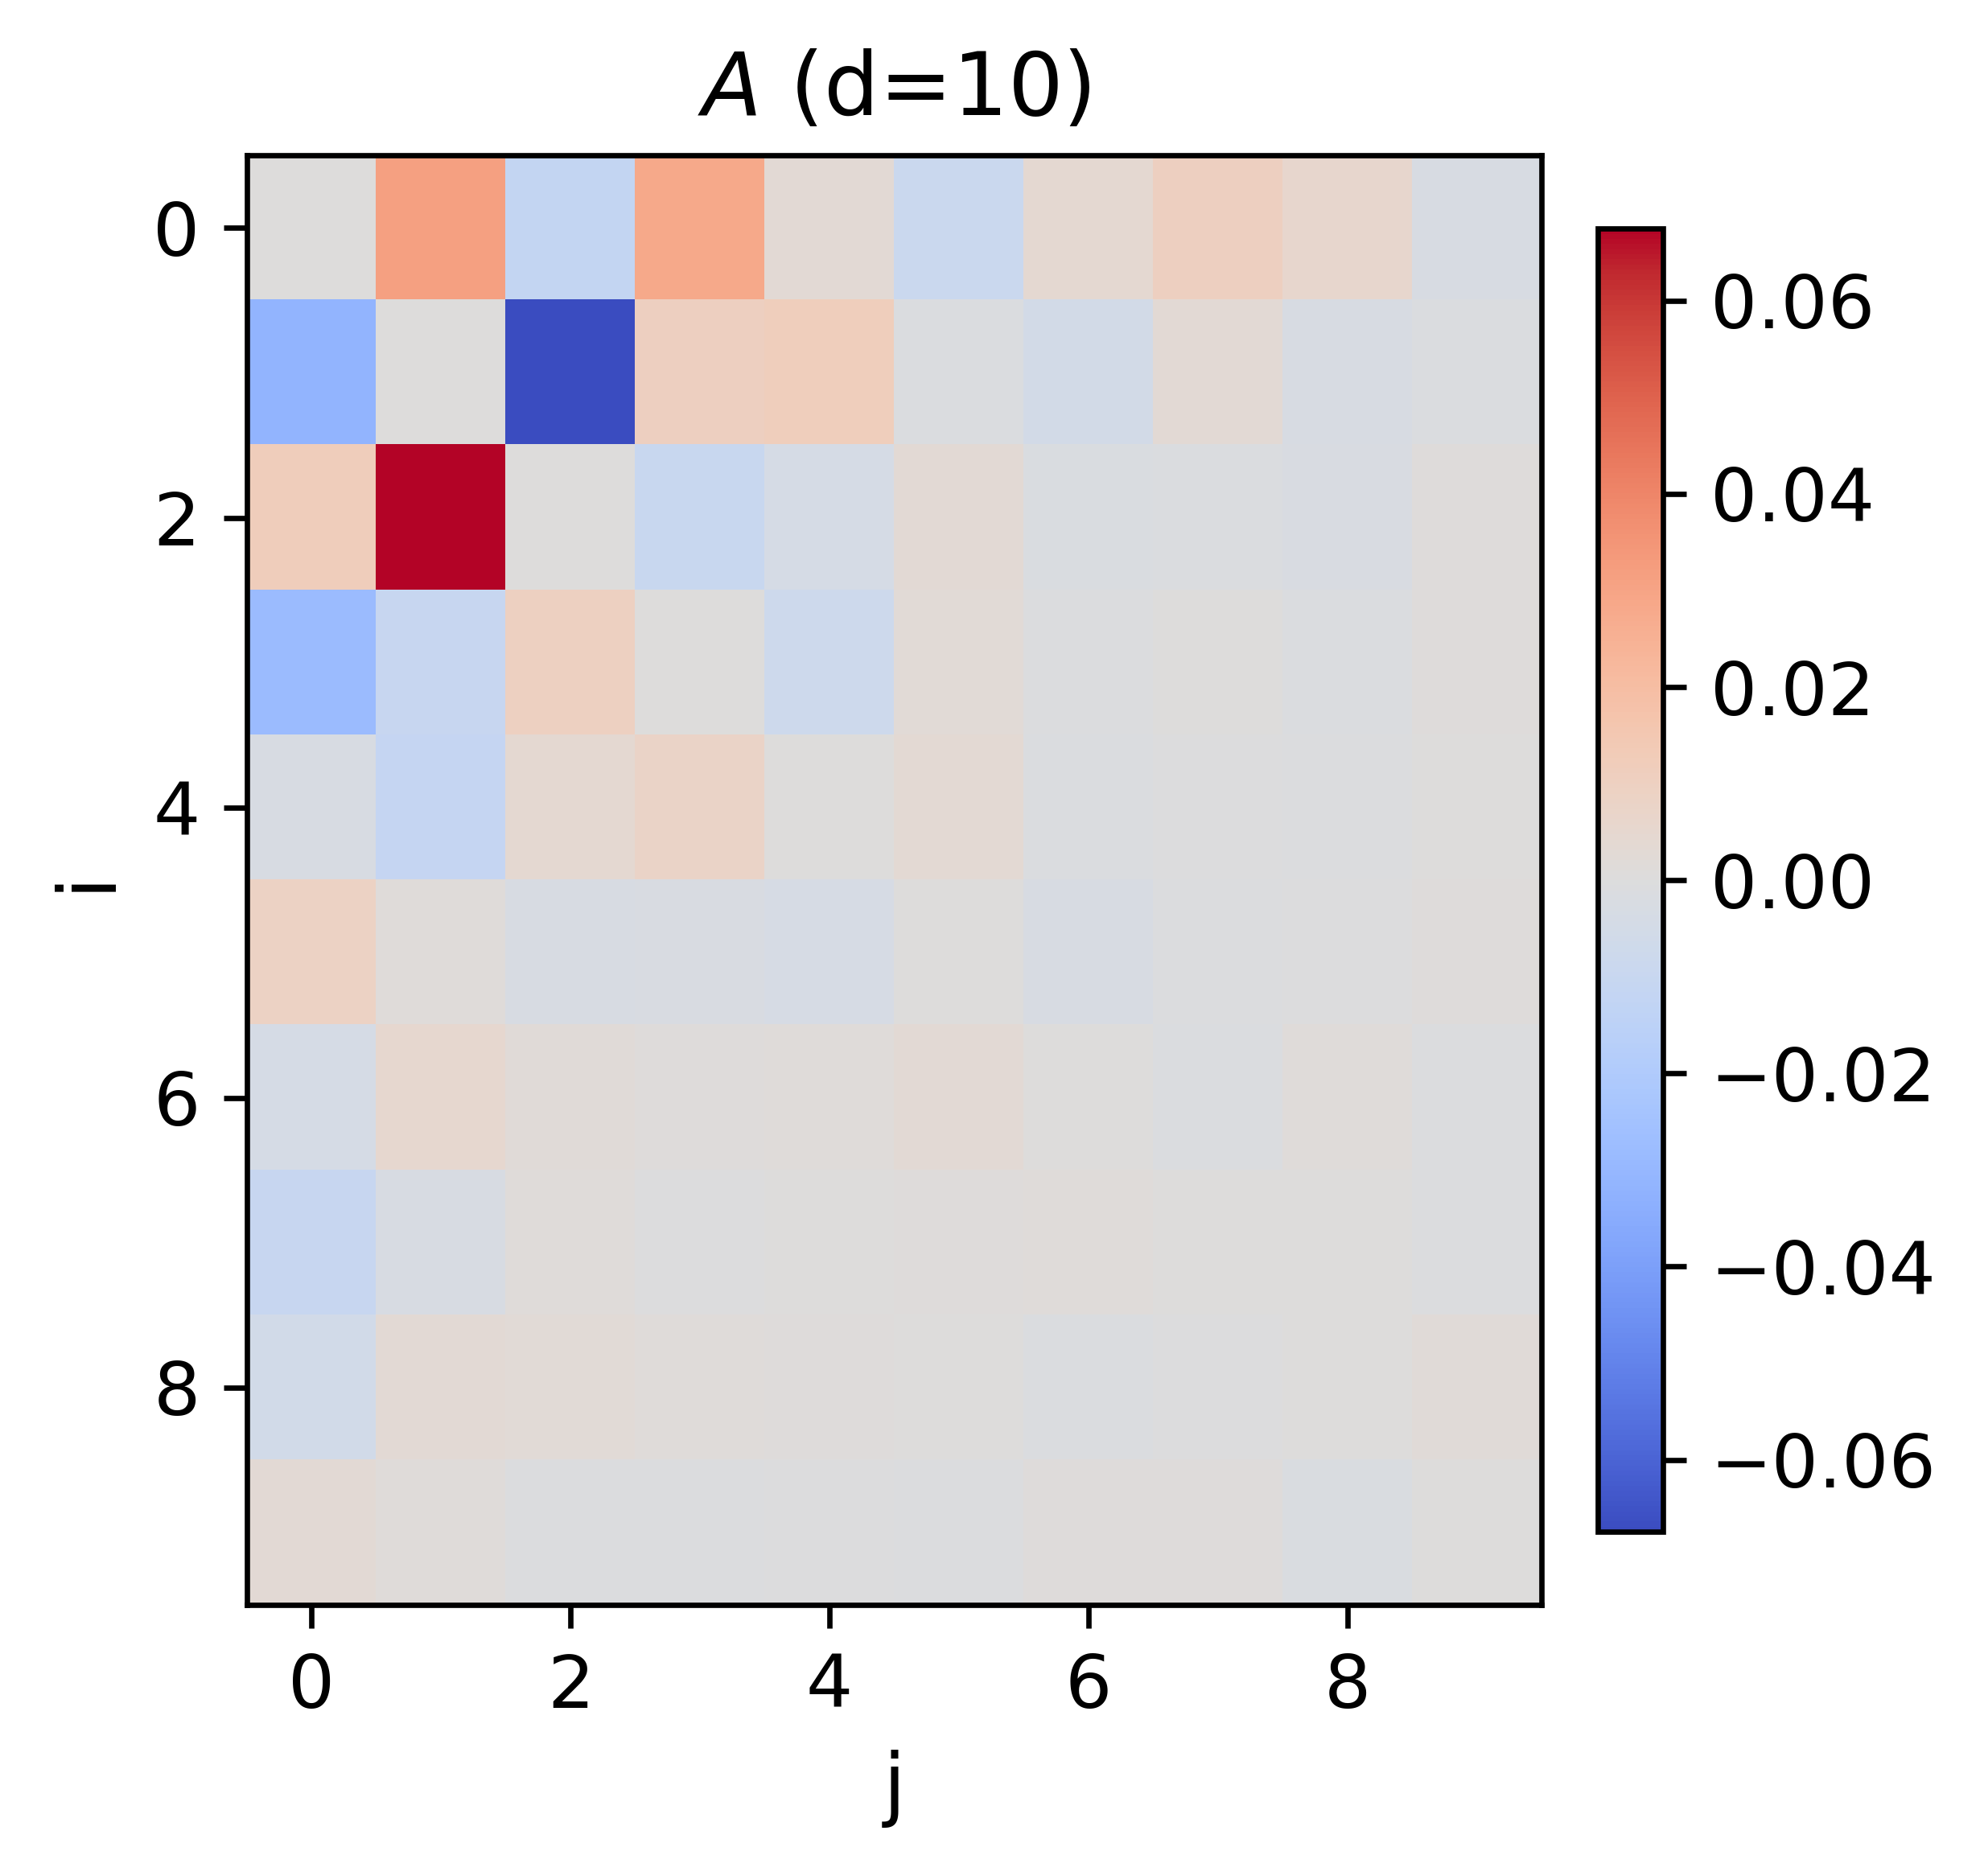
\includegraphics[width=\linewidth, trim={0 0 0 0.8cm}, clip]{visual_check_A_d10.png}
%         \caption{$A_{10}$.}
%     \end{subfigure}
%     \vfill
%     % \vspace{1cm}
%     \begin{subfigure}[b]{0.6\linewidth}
%         \centering
%         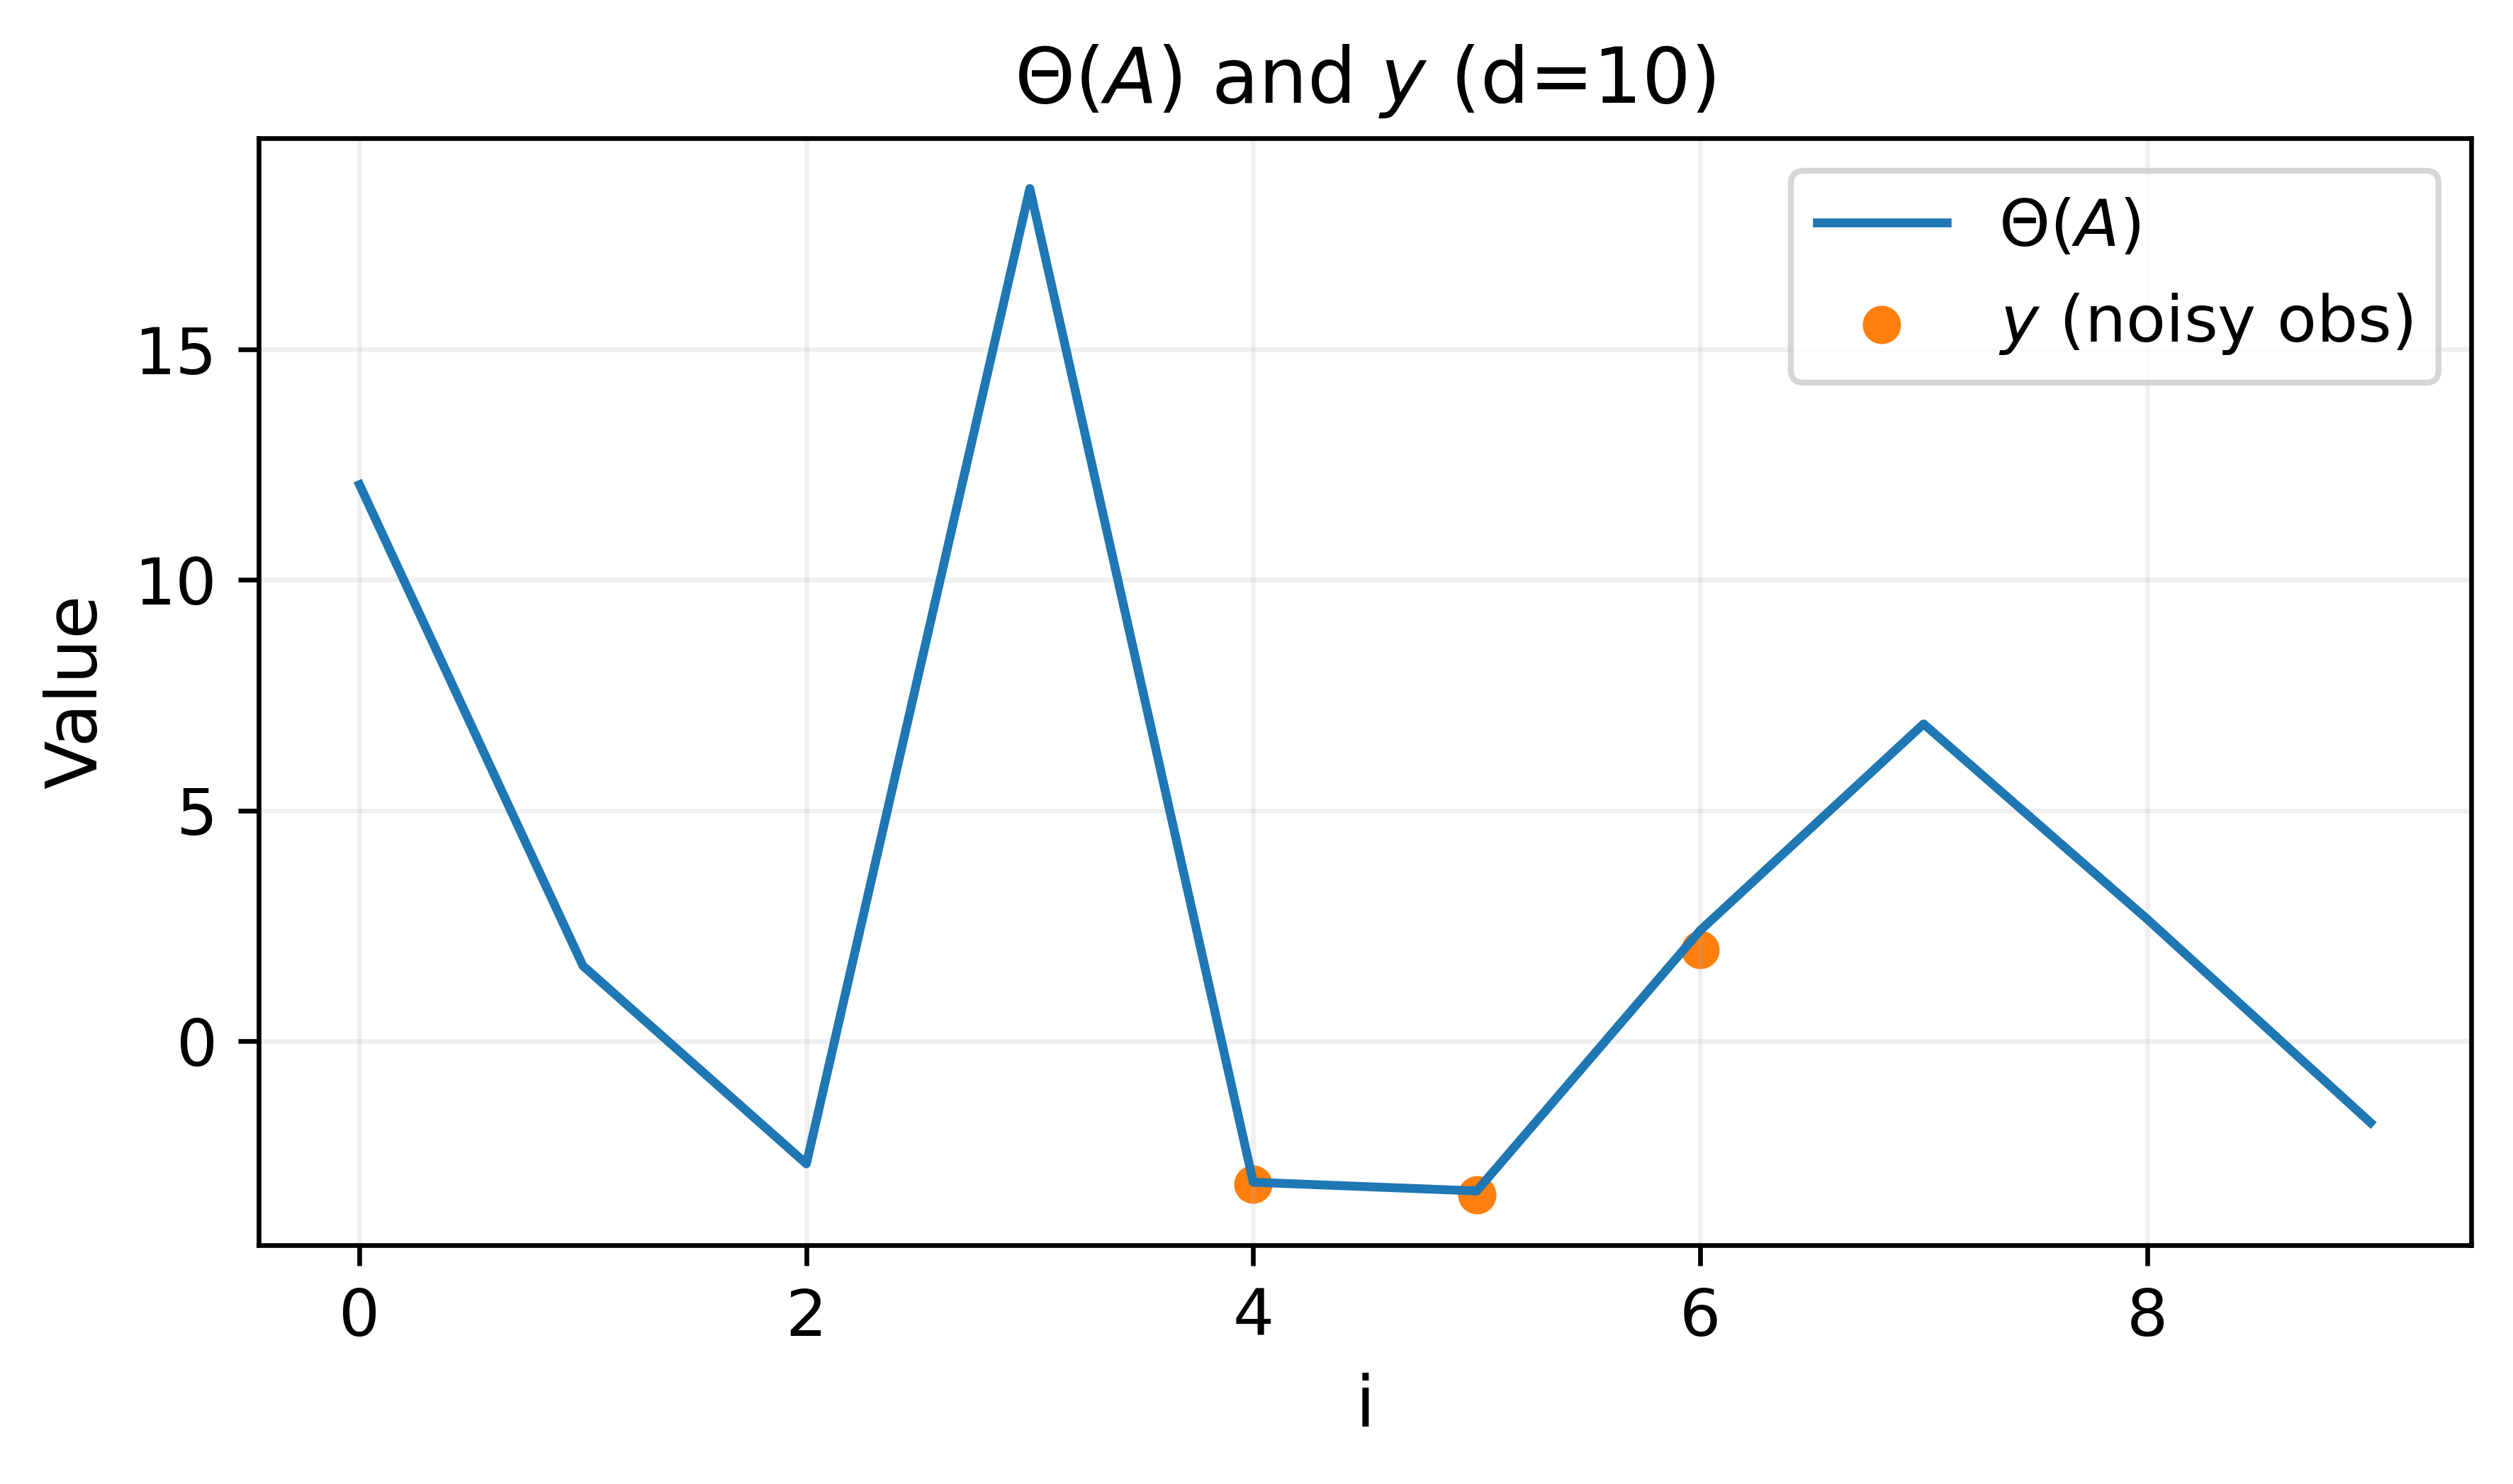
\includegraphics[width=\linewidth, trim={0 0 0 0.8cm}, clip]{visual_check_theta_y_d10.png}
%         \caption{$\Theta(A_{10})$ and $\mathsf{y}_3$.}
%     \end{subfigure}
% \end{figure}
% \end{column}
% \end{columns}
% \end{frame}

% \begin{frame}{Simulations from the model}
% \begin{figure}
%     \centering
%     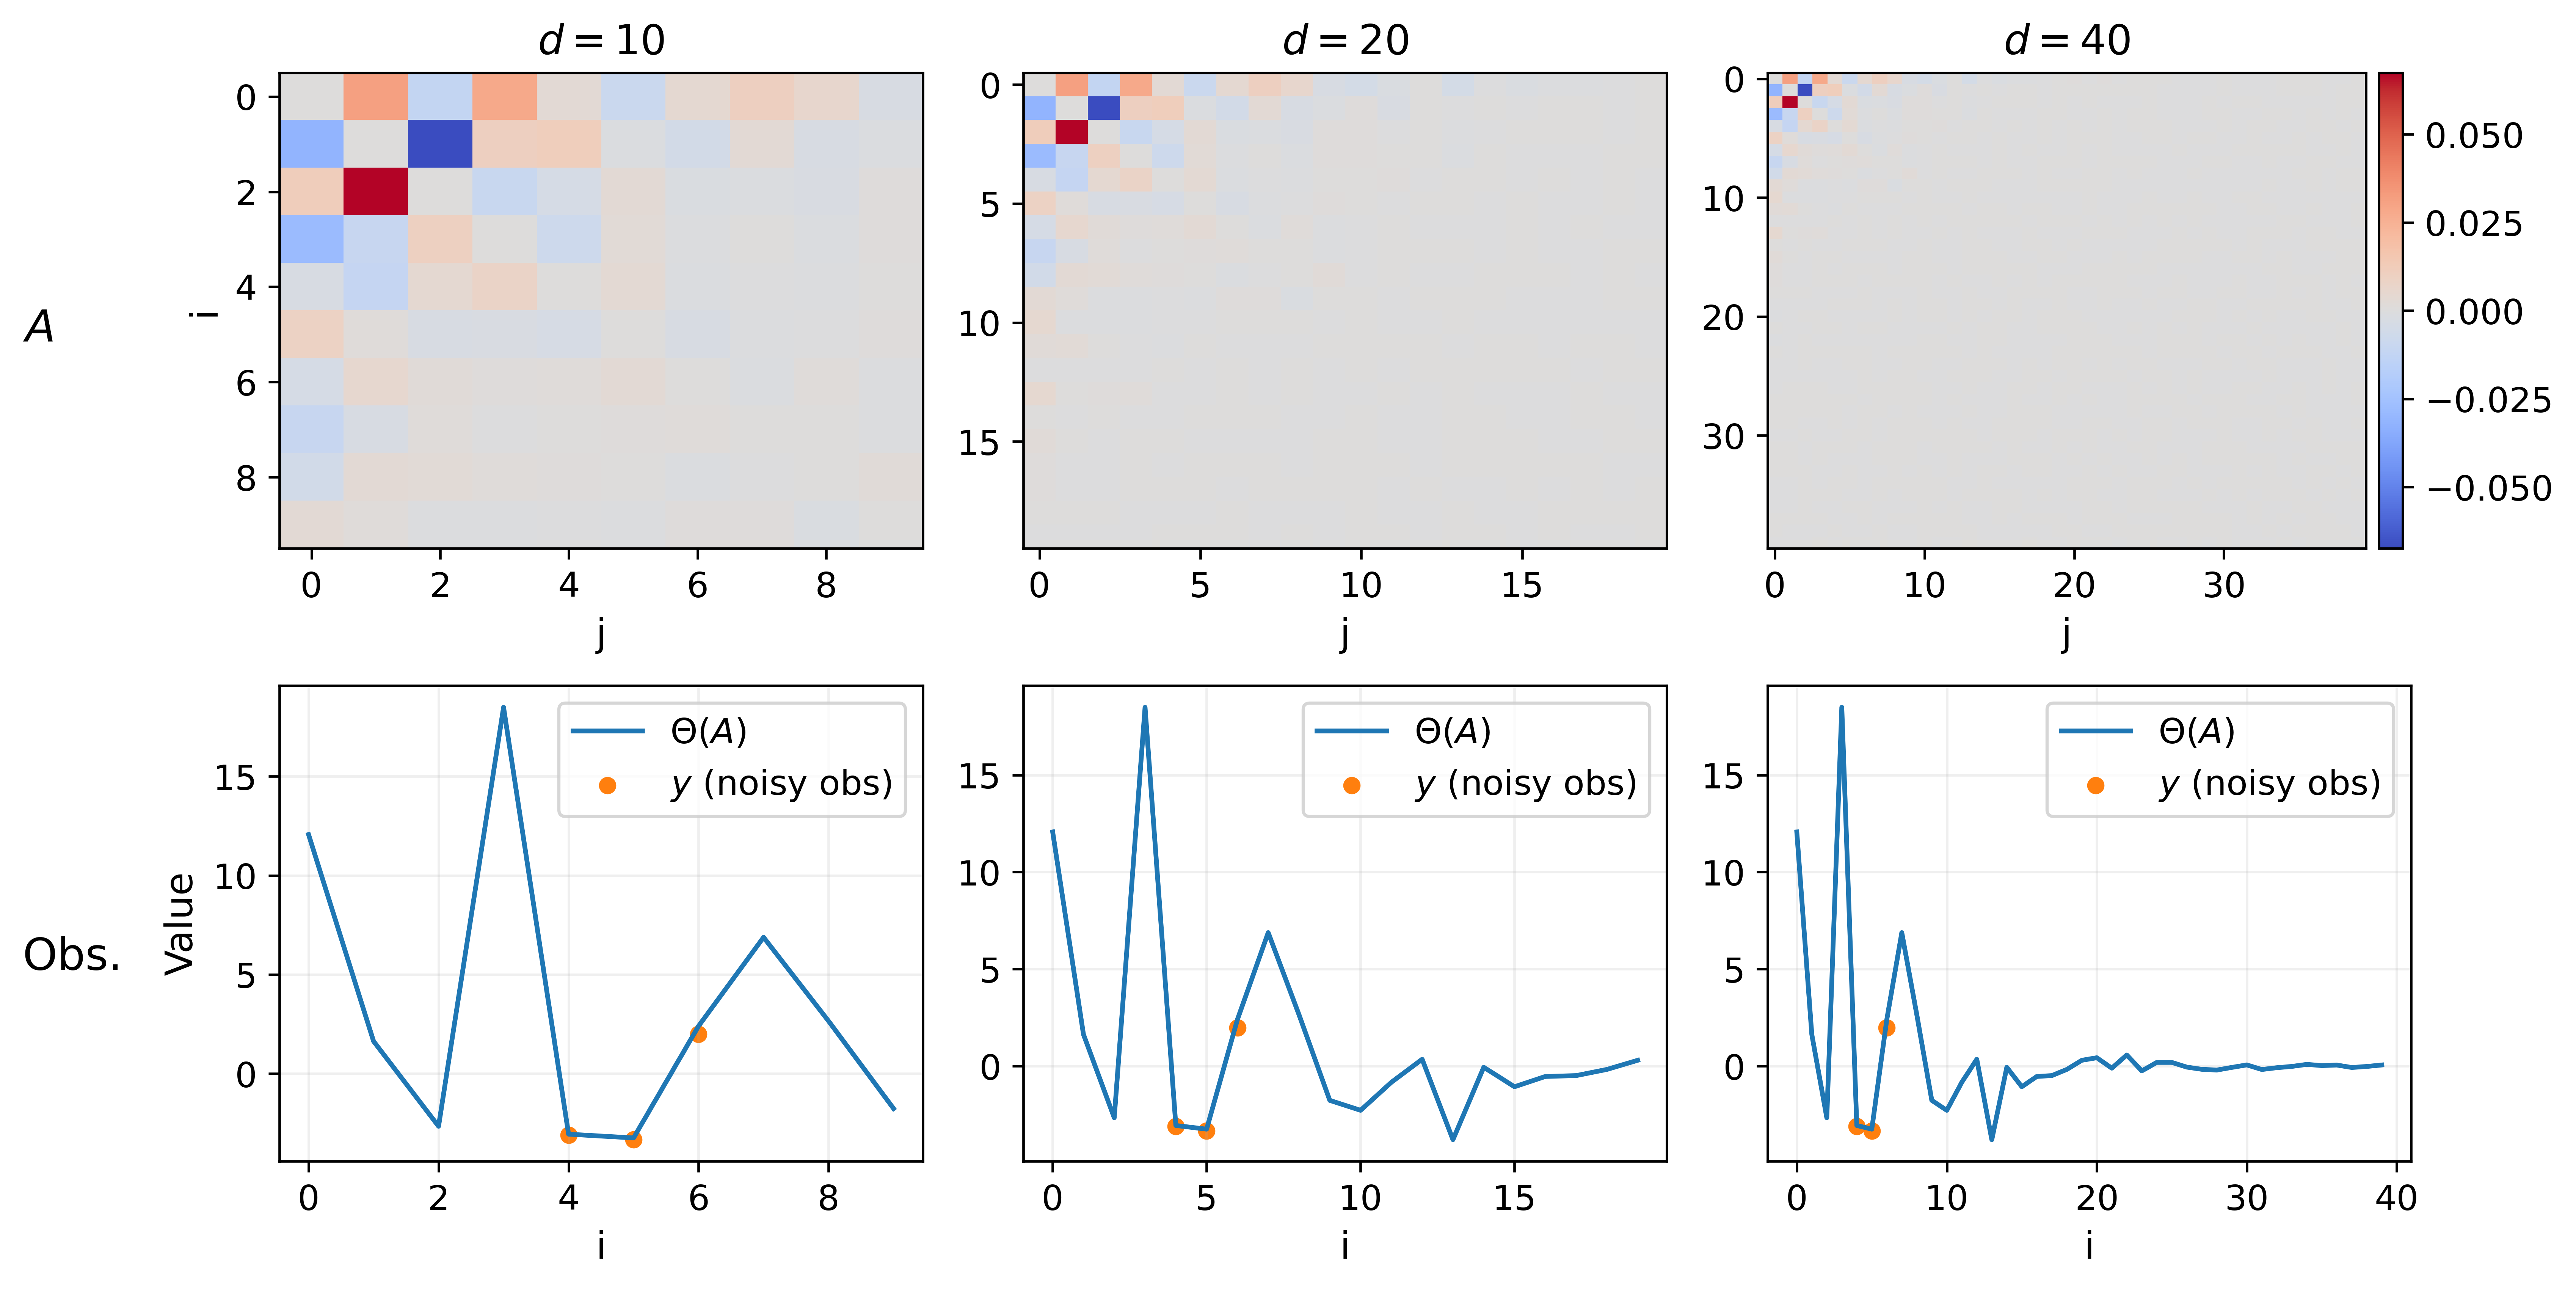
\includegraphics[width=0.75\linewidth]{visual_check_A_theta_y.png}
%     \caption{Toy solute transport: simulated $\bm{A}$, $\bm{\Theta}$, and observations.}
% \end{figure}
% \end{frame}

\begin{frame}{Posterior distribution for $d=10$}
\vspace{-0.5cm}
\begin{figure}
\centering
\begin{subfigure}[b]{0.4\linewidth}
    \centering
    \includegraphics[width=0.85\linewidth]{pairplot_algmess_d10_M100_n3.png}
    \caption{Some marginals and pairwise densities.}
\end{subfigure}
% \pause
\hfill
\begin{subfigure}[b]{0.55\linewidth}
    \vspace{-3cm}
    \centering
    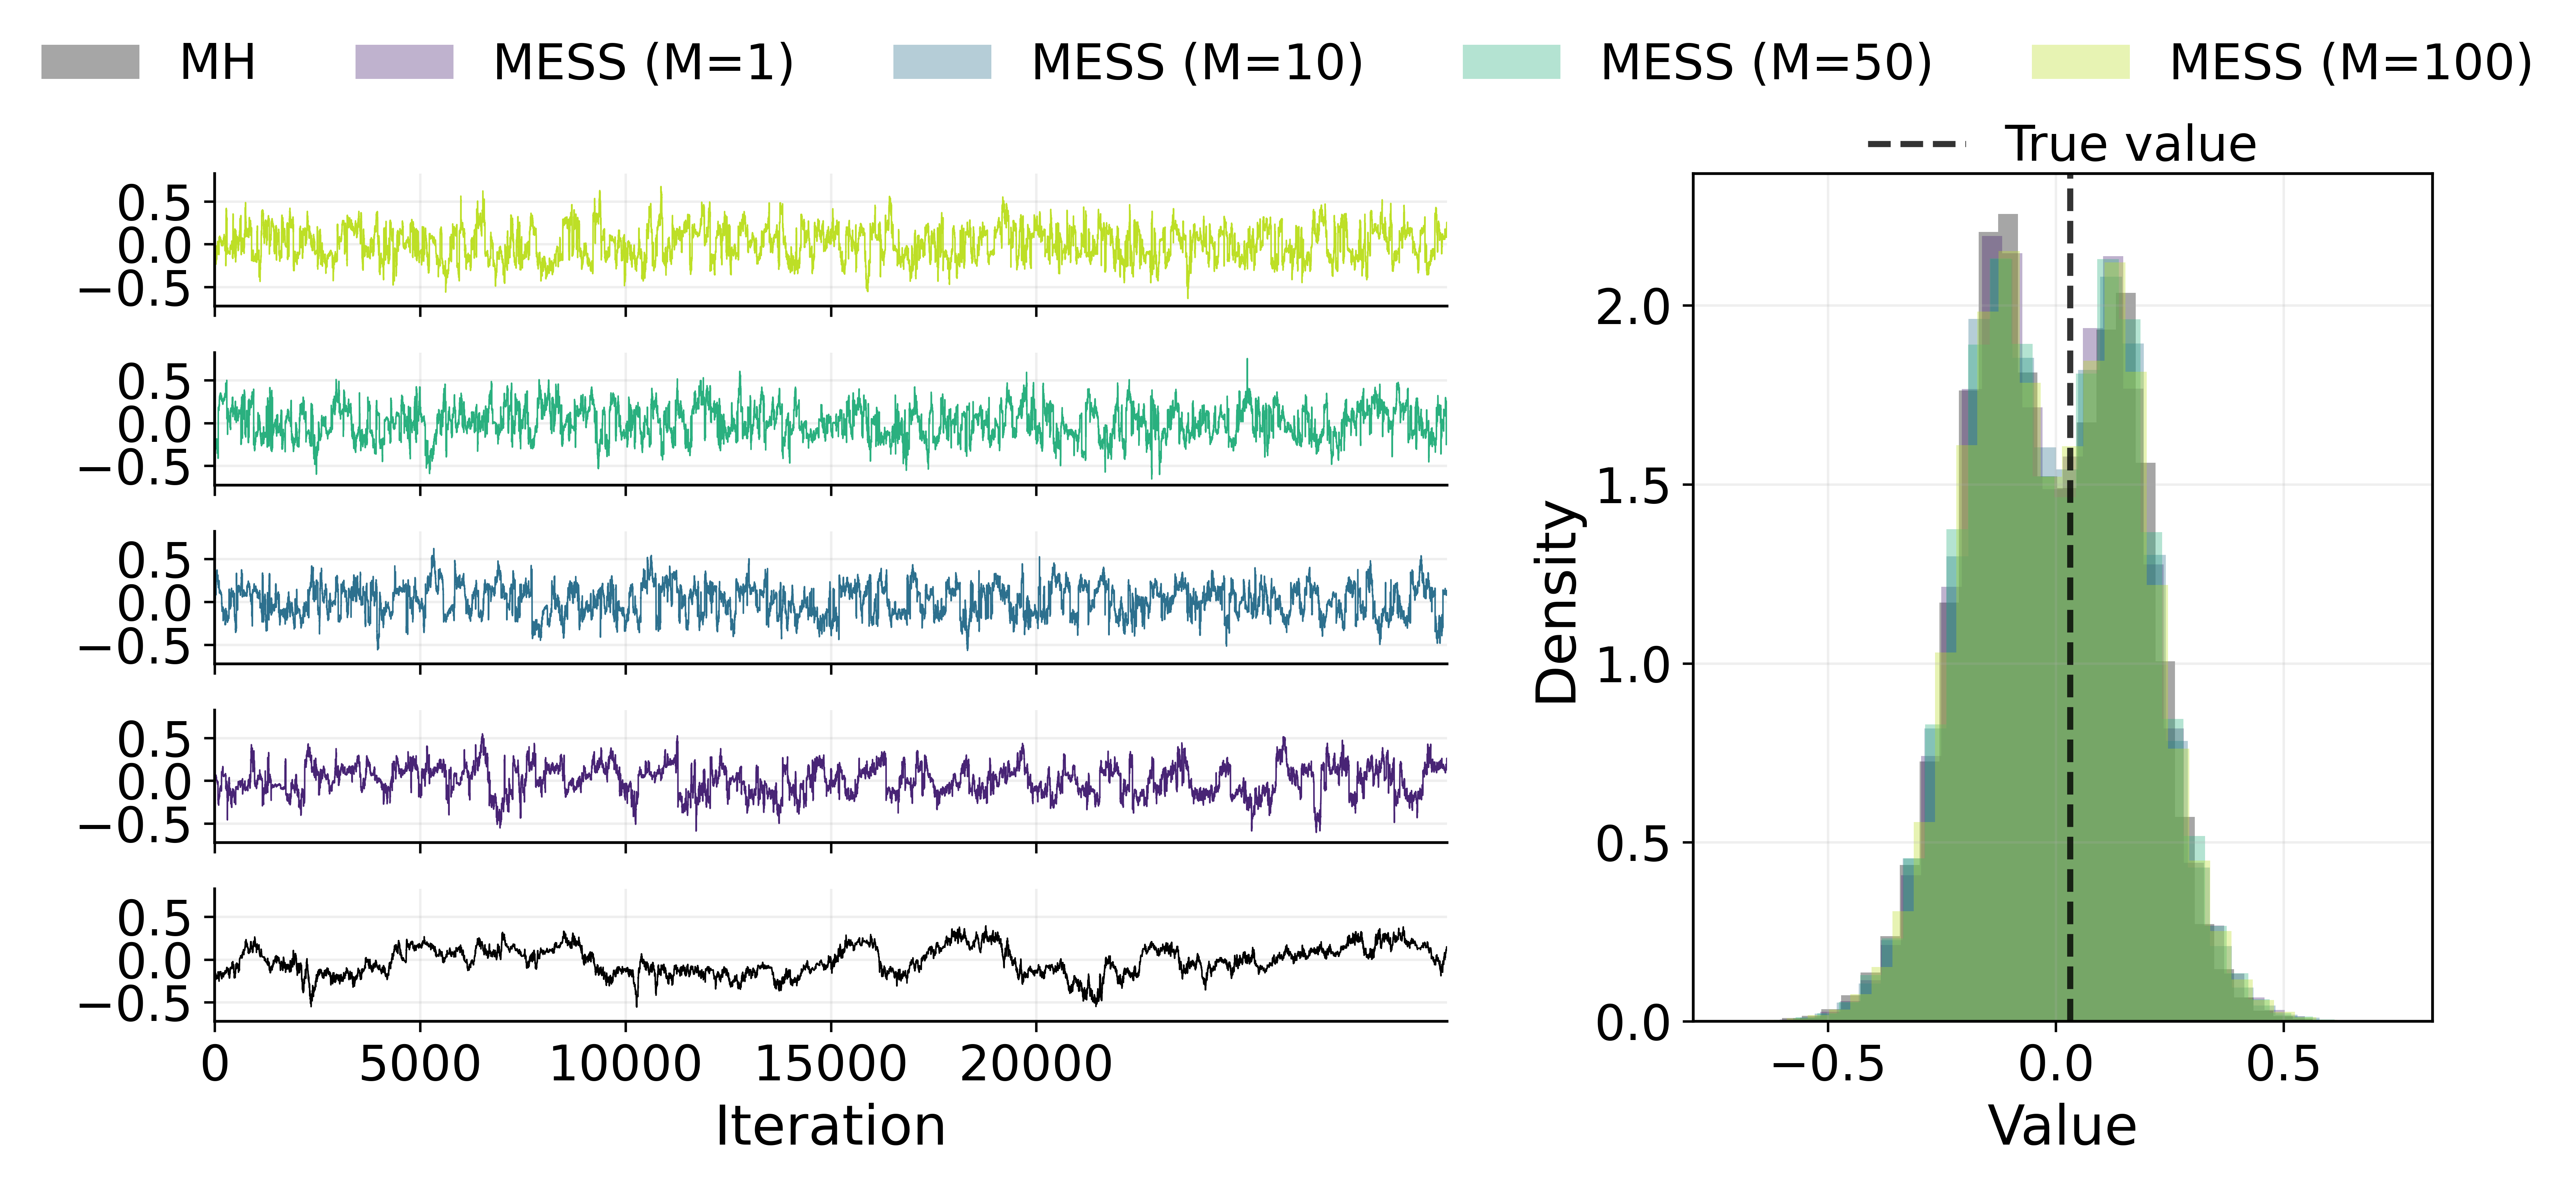
\includegraphics[width=\linewidth]{trace_hist_d10_comp0.png}
    \caption{Chain realizations for $a_{01}$.}
\end{subfigure}
% \caption{Posterior marginals and pairwise density plots at $d=10$.}
\end{figure}
\end{frame}

\begin{frame}{Dimension-free behavior}
\begin{figure}
    \centering
    \includegraphics[width=0.7\linewidth]{ess_msjd_vs_d_mean_log.png}
    \caption{MESS mixing rate does not degrade with dimension.}
\end{figure}
\end{frame}

% --------------------------------
\section{Conclusions}

\begin{frame}{Conclusions}
\vfill
\centering
Multiproposal Elliptical Slice Sampling (MESS) is\\[0.4em]
\textcolor{blue}{Self-tuning}\\[0.25em]
\textcolor{red}{no gradients}\\[0.25em]
\textcolor{green}{dimension-robust}\\[0.25em]
\textcolor{orange}{parallelizable}.\\
\vspace{0.1cm}
Useful for large-scale and/or non-parametric Bayesian estimation with Gaussian priors.
\vfill
\begin{figure}
\begin{subfigure}[b]{0.2\linewidth}
    \centering
    
\includegraphics[width=\linewidth, trim={0 5cm 0 0}, clip]{arxiv_mess.png}
    % \caption{arXiv}
\end{subfigure}
\hfill
\begin{subfigure}[b]{0.2\linewidth}
    \centering
    
\includegraphics[width=\linewidth, trim={0 5cm 0 0}, clip]{github_mess.png}
    % \caption{GitHub}
\end{subfigure} 
\end{figure}
% Outlook:
% \begin{itemize}[<+->]
%     % \item Cheaper approximations of the transition-matrix.
%     \item Convergence bounds via weak Harris theorem.
%     \item Test on large-scale Bayesian PDE inverse problems.
% \end{itemize}
\end{frame}

% \begin{frame}[allowframebreaks]{References}
% \bibliographystyle{chicago}
% \bibliography{references}
% \end{frame}

\miniframesoff
\begin{frame}[allowframebreaks]{References}
\bibliography{references}
\end{frame}
\miniframeson

% --------------------------------
\appendix
\section*{Supplementary}
\begin{frame}{Comparison with Gibbs and HMC: blind deconvolution inverse problem}
\begin{itemize}
    \item Observation model:
    \[
        d = w \star c + e, \quad w \sim N(0, C_w), \quad c \sim N(0, C_c), \quad e \sim N(0, C_e).
    \]
    \item Posterior is multimodal (sign-shift symmetry).
\end{itemize}
\vspace{0.3em}
\begin{figure}
    \centering
    \includegraphics[width=0.7\linewidth]{bd_blur_traceplots_posterior.jpeg}
    \caption{MESS explores both modes in 6m, HMC in 2.5hrs.}
\end{figure}
\end{frame}

\end{document}
